\documentclass{report}
%%%%%%%%%%%%%% preamble.tex %%%%%%%%%%%%%%
\usepackage[T1]{fontenc}
\usepackage{etoolbox}
% Page Setup
\usepackage[letterpaper, tmargin=2cm, rmargin=0.5in, lmargin=0.5in, bmargin=80pt, footskip=.2in]{geometry}
\usepackage{adjustbox}
\usepackage{graphicx}
\usepackage{tikz}
\usepackage{mathrsfs}
\usepackage{mdframed}

% Create a new toggle
\newtoggle{firstsection}

% Redefine the \chapter command to reset the toggle for each new chapter
\let\oldchapter\chapter
\renewcommand{\chapter}{\toggletrue{firstsection}\oldchapter}

% Redefine the \section command to check the toggle
\let\oldsection\section
\renewcommand{\section}{
    \iftoggle{firstsection}
    {\togglefalse{firstsection}} % If it's the first section, just switch off the toggle for next sections
    {\clearpage} % If it's not the first section, start a new page
    \oldsection
}

% Abstract Design

\usepackage{lipsum}

\renewenvironment{abstract}
 {% Start of environment
  \quotation
  \small
  \noindent
  \rule{\linewidth}{.5pt} % Draw the rule to match the linewidth
  \par\smallskip
  {\centering\bfseries\abstractname\par}\medskip
 }
 {% End of environment
  \par\noindent
  \rule{\linewidth}{.5pt} % Ensure the closing rule also matches
  \endquotation
 }

% Mathematics
\usepackage{amsmath,amsfonts,amsthm,amssymb,mathtools}
\usepackage{xfrac}
\usepackage[makeroom]{cancel}
\usepackage{enumitem}
\usepackage{nameref}
\usepackage{multicol,array}
\usepackage{tikz-cd}
\usepackage{array}
\usepackage{multirow}% http://ctan.org/pkg/multirow
\usepackage{graphicx}

% Colors
\usepackage[dvipsnames]{xcolor}
\definecolor{myg}{RGB}{56, 140, 70}
\definecolor{myb}{RGB}{45, 111, 177}
\definecolor{myr}{RGB}{199, 68, 64}
% Define more colors here...
\definecolor{olive}{HTML}{6B8E23}
\definecolor{orange}{HTML}{CC5500}
\definecolor{brown}{HTML}{8B4513}
% Hyperlinks
\usepackage{bookmark}
\usepackage[colorlinks=true,linkcolor=blue,urlcolor=blue,citecolor=blue,anchorcolor=blue]{hyperref}
\usepackage{xcolor}
\hypersetup{
    colorlinks,
    linkcolor={red!50!black},
    citecolor={blue!50!black},
    urlcolor={blue!80!black}
}

% Text-related
\usepackage{blindtext}
\usepackage{fontsize}
\changefontsize[14]{14}
\setlength{\parindent}{0pt}
\linespread{1.2}

% Theorems and Definitions
\usepackage{amsthm}
\renewcommand\qedsymbol{$\blacksquare$}

% Define a new theorem style
\newtheoremstyle{mytheoremstyle}% name
  {}% Space above
  {}% Space below
  {}% Body font
  {}% Indent amount
  {\bfseries}% Theorem head font
  {.}% Punctuation after theorem head
  {.5em}% Space after theorem head
  {}% Theorem head spec (can be left empty, meaning ‘normal’)

% Apply the new theorem style to theorem-like environments
\theoremstyle{mytheoremstyle}

\newtheorem{theorem}{Theorem}[section]  
\newtheorem{definition}[theorem]{Definition} 
\newtheorem{lemma}[theorem]{Lemma}  
\newtheorem{corollary}[theorem]{Corollary}
\newtheorem{axiom}[theorem]{Axiom}
\newtheorem{example}[theorem]{Example}
\newtheorem{equiv_def}[theorem]{Equivalent Definition}

% tcolorbox Setup
\usepackage[most,many,breakable]{tcolorbox}
\tcbuselibrary{theorems}

% Define custom tcolorbox environments here...

%================================
% EXAMPLE BOX
%================================
% After you have defined the style and other theorem environments
\definecolor{myexamplebg}{RGB}{245, 245, 245} % Very light grey for background
\definecolor{myexamplefr}{RGB}{120, 120, 120} % Medium grey for frame
\definecolor{myexampleti}{RGB}{60, 60, 60}    % Darker grey for title

\newtcbtheorem[]{Example}{Example}{
    colback=myexamplebg,
    breakable,
    colframe=myexamplefr,
    coltitle=myexampleti,
    boxrule=1pt,
    sharp corners,
    detach title,
    before upper=\tcbtitle\par\vspace{-20pt}, % Reduced the space after the title
    fonttitle=\bfseries,
    description font=\mdseries,
    separator sign none,
    description delimiters={}{}, % No delimiters around the title
}{ex}
%================================
% Solution BOX
%================================
\makeatletter
\newtcolorbox{solution}{enhanced,
	breakable,
	colback=white,
	colframe=myg!80!black,
	attach boxed title to top left={yshift*=-\tcboxedtitleheight},
	title=Solution,
	boxed title size=title,
	boxed title style={%
			sharp corners,
			rounded corners=northwest,
			colback=tcbcolframe,
			boxrule=0pt,
		},
	underlay boxed title={%
			\path[fill=tcbcolframe] (title.south west)--(title.south east)
			to[out=0, in=180] ([xshift=5mm]title.east)--
			(title.center-|frame.east)
			[rounded corners=\kvtcb@arc] |-
			(frame.north) -| cycle;
		},
}
\makeatother

% %================================
% % Question BOX
% %================================
\makeatletter
\newtcbtheorem{question}{Question}{enhanced,
	breakable,
	colback=white,
	colframe=myb!80!black,
	attach boxed title to top left={yshift*=-\tcboxedtitleheight},
	fonttitle=\bfseries,
	title={#2},
	boxed title size=title,
	boxed title style={%
			sharp corners,
			rounded corners=northwest,
			colback=tcbcolframe,
			boxrule=0pt,
		},
	underlay boxed title={%
			\path[fill=tcbcolframe] (title.south west)--(title.south east)
			to[out=0, in=180] ([xshift=5mm]title.east)--
			(title.center-|frame.east)
			[rounded corners=\kvtcb@arc] |-
			(frame.north) -| cycle;
		},
	#1
}{question}
\makeatother

%%%%%%%%%%%%%%%%%%%%%%%%%%%%%%%%%%%%%%%%%%%
% TABLE OF CONTENTS
%%%%%%%%%%%%%%%%%%%%%%%%%%%%%%%%%%%%%%%%%%%


\usepackage{tikz}
\definecolor{doc}{RGB}{0,60,110}
\usepackage{titletoc}
\contentsmargin{0cm}
\titlecontents{chapter}[14pc]
{\addvspace{30pt}%
	\begin{tikzpicture}[remember picture, overlay]%
		\draw[fill=doc!60,draw=doc!60] (-7,-.1) rectangle (-0.9,.5);%
		\pgftext[left,x=-5.5cm,y=0.2cm]{\color{white}\Large\sc\bfseries Chapter\ \thecontentslabel};%
	\end{tikzpicture}\color{doc!60}\large\sc\bfseries}%
{}
{}
{\;\titlerule\;\large\sc\bfseries Page \thecontentspage
	\begin{tikzpicture}[remember picture, overlay]
		\draw[fill=doc!60,draw=doc!60] (2pt,0) rectangle (4,0.1pt);
	\end{tikzpicture}}%
\titlecontents{section}[3.7pc]
{\addvspace{2pt}}
{\contentslabel[\thecontentslabel]{3pc}}
{}
{\hfill\small \thecontentspage}
[]
\titlecontents*{subsection}[3.7pc]
{\addvspace{-1pt}\small}
{}
{}
{\ --- \small\thecontentspage}
[ \textbullet\ ][]

\makeatletter
\renewcommand{\tableofcontents}{
	\chapter*{%
	  \vspace*{-20\p@}%
	  \begin{tikzpicture}[remember picture, overlay]%
		  \pgftext[right,x=15cm,y=0.2cm]{\color{doc!60}\Huge\sc\bfseries \contentsname};%
		  \draw[fill=doc!60,draw=doc!60] (13,-.75) rectangle (20,1);%
		  \clip (13,-.75) rectangle (20,1);
		  \pgftext[right,x=15cm,y=0.2cm]{\color{white}\Huge\sc\bfseries \contentsname};%
	  \end{tikzpicture}}%
	\@starttoc{toc}}
\makeatother

\newcommand{\liff}{\llap{$\iff$}}
\newcommand{\rap}[1]{\rrap{\text{ (#1)}}}
\newcommand{\red}[1]{\textcolor{red}{#1}}
\newcommand{\blue}[1]{\textcolor{blue}{#1}}
\newcommand{\vi}[1]{\textcolor{violet}{#1}}
\newcommand{\olive}[1]{\textcolor{olive}{#1}}
\newcommand{\teal}[1]{\textcolor{teal}{#1}}
\newcommand{\brown}[1]{\textcolor{brown}{#1}}
\newcommand{\orange}[1]{\textcolor{orange}{#1}}
\newcommand{\tCaC}{\text{ \CaC }}
\newcommand{\CaC}{\red{CaC} }
\newcommand{\As}[1]{Assume \red{#1}}
\newcommand{\vdone}{\vi{\text{ (done) }}}
\newcommand{\bdone}{\blue{\text{ (done) }}}
\newcommand{\tdone}{\teal{\text{ (done) }}}
\newcommand{\odone}{\olive{\text{ (done) }}}
\newcommand{\bodone}{\brown{\text{ (done) }}}
\newcommand{\ordone}{\orange{\text{ (done) }}}
\newcommand{\ld}{\lambda}
\newcommand{\vecta}[1]{\textbf{#1}}
\newcommand{\set}[1]{\left\{ #1 \right\}}
\newcommand{\bset}[1]{\Big\{ #1 \Big\}}
\newcommand{\inR}{\in\R}
\newcommand{\inn}{\in\N}
\newcommand{\inz}{\in\Z}
\newcommand{\inr}{\in\R}
\newcommand{\inc}{\in\C}
\newcommand{\inq}{\in\Q}
\newcommand{\norm}[1]{\| #1 \|}
\newcommand{\bnorm}[1]{\Big\| #1 \Big\|}
\newcommand{\gen}[1]{\langle #1 \rangle}
\newcommand{\abso}[1]{\left|#1\right|}
\newcommand{\myref}[2]{\hyperref[#2]{#1\ \ref*{#2}}}
\newcommand{\customref}[2]{\hyperref[#1]{#2}}
\newcommand{\power}[1]{\mathcal{P}(#1)}
\newcommand{\dcup}{\mathbin{\dot{\cup}}}
\newcommand{\diam}[1]{\text{diam}\, #1}
\newcommand{\at}{\Big|}
\newcommand{\quotient}{\diagup}
\let\originalphi\phi % Store the original \phi in \originalphi
\renewcommand{\phi}{\varphi} % Redefine \phi to \varphi
\newcommand{\pfi}{\originalphi} % Define \pfi to display the original \phi
\newcommand{\diota}{\dot{\iota}}
\newcommand{\Log}{\operatorname{Log}}
\newcommand{\id}{\text{\textbf{id}}}
\usepackage{amsmath}

\makeatletter
\NewDocumentCommand{\extp}{e{^}}{%
  \mathop{\mathpalette\extp@{#1}}\nolimits
}
\NewDocumentCommand{\extp@}{mm}{%
  \bigwedge\nolimits\IfValueT{#2}{^{\extp@@{#1}#2}}%
  \IfValueT{#1}{\kern-2\scriptspace\nonscript\kern2\scriptspace}%
}
\newcommand{\extp@@}[1]{%
  \mkern
    \ifx#1\displaystyle-1.8\else
    \ifx#1\textstyle-1\else
    \ifx#1\scriptstyle-1\else
    -0.5\fi\fi\fi
  \thinmuskip
}
\makeatletter
\usepackage{pifont}
\makeatletter
\newcommand\Pimathsymbol[3][\mathord]{%
  #1{\@Pimathsymbol{#2}{#3}}}
\def\@Pimathsymbol#1#2{\mathchoice
  {\@Pim@thsymbol{#1}{#2}\tf@size}
  {\@Pim@thsymbol{#1}{#2}\tf@size}
  {\@Pim@thsymbol{#1}{#2}\sf@size}
  {\@Pim@thsymbol{#1}{#2}\ssf@size}}
\def\@Pim@thsymbol#1#2#3{%
  \mbox{\fontsize{#3}{#3}\Pisymbol{#1}{#2}}}
\makeatother
% the next two lines are needed to avoid LaTeX substituting upright from another font
\input{utxmia.fd}
\DeclareFontShape{U}{txmia}{m}{n}{<->ssub * txmia/m/it}{}
% you may also want
\DeclareFontShape{U}{txmia}{bx}{n}{<->ssub * txmia/bx/it}{}
% just in case
%\DeclareFontShape{U}{txmia}{l}{n}{<->ssub * txmia/l/it}{}
%\DeclareFontShape{U}{txmia}{b}{n}{<->ssub * txmia/b/it}{}
% plus info from Alan Munn at https://tex.stackexchange.com/questions/290165/how-do-i-get-a-nicer-lambda?noredirect=1#comment702120_290165
\newcommand{\pilambdaup}{\Pimathsymbol[\mathord]{txmia}{21}}
\renewcommand{\lambda}{\pilambdaup}
\renewcommand{\tilde}{\widetilde}
\DeclareMathOperator*{\esssup}{ess\,sup}
\newcommand{\bluecheck}{}%
\DeclareRobustCommand{\bluecheck}{%
  \tikz\fill[scale=0.4, color=blue]
  (0,.35) -- (.25,0) -- (1,.7) -- (.25,.15) -- cycle;%
}


\usepackage{tikz}
\newcommand*{\DashedArrow}[1][]{\mathbin{\tikz [baseline=-0.25ex,-latex, dashed,#1] \draw [#1] (0pt,0.5ex) -- (1.3em,0.5ex);}}

\newcommand{\C}{\mathbb{C}}	
\newcommand{\F}{\mathbb{F}}
\newcommand{\N}{\mathbb{N}}
\newcommand{\Q}{\mathbb{Q}}
\newcommand{\R}{\mathbb{R}}
\newcommand{\Z}{\mathbb{Z}}



\title{\Huge{NCKU 112.2}\\
Miscellaneous Facts}
\author{\huge{Eric Liu}}
\date{}
\begin{document}
\maketitle
\newpage% or \cleardoublepage
% \pdfbookmark[<level>]{<title>}{<dest>}
\pdfbookmark[section]{\contentsname}{toc}
\tableofcontents
\pagebreak

\chapter{General Topology}
\section{Directed Sets}
\begin{axiom}
\label{1.1.1}
\textbf{(Axioms in Order Theory)} Given an relation $(X,\leq )$, and suppose  $x,y,z \in X$. 
\begin{enumerate}[label=(\alph*)]
  \item $x\leq x$ (Reflexive)
  \item $x\leq y\leq z \implies x\leq z$ (Transitive)
  \item $x\leq y\text{ and }y\leq x\implies x=y$ (Antisymmetric)
  \item $x\leq y\text{ or }y\leq x$ (Connected)
  \item $\forall x,y \in X, \exists z\in X, x\leq z\text{ and }y\leq z$ (Directed)
\end{enumerate}
We say $(X,\leq )$ form a 
\begin{enumerate}[label=(\alph*)]
  \item \red{total order} if it is reflexive, transitive, antisymmetric and connected. 
  \item \red{partial order} if it is reflexive, transitive and  antisymmetric. 
  \item \red{preorder} if it is reflexive and transitive.
  \item \red{directed set} if it is reflexive, transitive and directed. 
\end{enumerate}
\end{axiom}
\begin{theorem}
\label{1.1.2}
\textbf{(Why is it called Preorder)} Given a preorder $(X,\leq )$, the relation $\sim$ defined by 
\begin{align*}
x\sim y \iff x\leq y\text{ and }y\leq x
\end{align*}
is an equivalence relation and if we define $\leq^e$ on the equivalence class by 
\begin{align*}
\exists x \in A, y \in B, x\leq y \implies A\leq^e B
\end{align*}
Then $\leq^e$ is a partial order. Moreover, if the preorder $\leq $ is directed, then $\leq ^e$ is also directed.
\end{theorem}
\begin{proof}
We first show \vi{$\sim$ is an equivalence relation}. Because preoder is reflexive, we see 
\begin{align*}
\forall x\in X, x\leq x\text{ which implies }\forall x \in X, x \sim x
\end{align*}
For symmetry, it is easy to see 
\begin{align*}
x\sim y \implies x\leq y\text{ and }y\leq x\implies y\sim x
\end{align*}
For transitive, see 
\begin{align*}
  x\sim y \text{ and } y\sim z&\implies x\leq y \text{ and }y \leq x \text{ and }y\leq z \text{ and }z \leq y \\
&\implies x\leq z\text{ and } z\leq x\implies x\sim z \vdone
\end{align*}
We now show \blue{$\leq^e$ is a partial order}. Reflexive property and Transitive property of $\leq^e$ follow from that of $\leq $. Suppose $A\leq^e B$ and $B\leq^e A$, where $x_1,x_2\in A,y_1,y_2\in B$ satisfy $x_1\leq y_1$ and $y_2\leq x_2$. Because $x_1,x_2 \in A$ and $y_1,y_2\in B$, we have 
\begin{align*}
x_1\leq x_2\text{ and }x_2\leq x_1\text{ and }y_1\leq y_2\text{ and }y_2\leq y_1
\end{align*}
Then because $\leq $ satisfy transitive, we have 
\begin{align*}
\begin{cases}
  x_2\leq x_1\leq y_1 \implies x_2\leq y_1\\
  y_1\leq y_2\leq x_2 \implies y_1\leq x_2
\end{cases}
\end{align*}
This tell us 
\begin{align*}
x_2 \sim y_1
\end{align*}
which implies $A=B$, thus proving  $\leq^e$ is antisymmetirc. $\bdone$\\

Lastly, we show  \vi{$\leq $ is directed$\implies \leq ^e$ is directed}. Let $A,B$ be two arbitrary equivalence class. We wish to find an equivalence class $T$ such that 
\begin{align*}
A\leq^e T \text{ and } B\leq^e T
\end{align*}
Let $a,b$ respectively be an arbitrary element of $A,B$. Because  $\leq $ is directed, we know there exists $c\in X$ such that 
\begin{align*}
a\leq c\text{ and }b\leq c
\end{align*}
We immediately see 
\begin{align*}
A\leq^e [c] \text{ and } B\leq^e [c] \vdone
\end{align*}
\end{proof}
\begin{corollary}
\label{1.1.3}
\textbf{(Chunk Structure of Preorder)} Given two equivalence class $A,B$, we have
 \begin{align*}
A\leq^e B \implies \forall x\in A,y \in B, x\leq y
\end{align*}
\end{corollary}
\begin{proof}
Because $A\leq ^e B$, we know 
\begin{align*}
\exists x_0\in A,y_0\in B, x_0\leq y_0
\end{align*}
Then by definition of $\sim$, we have
\begin{align*}
x \leq x_0\leq y_0\leq y
\end{align*}
This give us 
\begin{align*}
x\leq y
\end{align*}
\end{proof}
\begin{definition}
\label{1.1.4}
\textbf{(Definition of Maximal element in Preorder)} Let $(I,\leq )$ be a preorder. We say $m\in I$ is a maximal element if 
\begin{align*}
\forall y\in I, m\leq y\implies y\leq m
\end{align*}
\end{definition}
\begin{theorem}
\label{1.1.5}
\textbf{(In Preorder, Maximal element form an Equivalence class)} Let $(I,\leq )$ be a preorder, and $m \in  I$ be a maximal element. Then 
\begin{align*} 
\forall x\in [m], x\text{ is a maximal element }
\end{align*}
\end{theorem}
\begin{proof}
Arbitrarily pick an element $x$ in $[m]$. Suppose 
\begin{align*}
x\leq y 
\end{align*}
By definition of $\sim$, we have 
\begin{align*}
m\leq x\leq y
\end{align*}
Thus $m\leq y$. Then because $m$ is maximal, we know $y\leq m$. This now give us 
\begin{align*}
y\leq m\leq x
\end{align*}
\end{proof}
\begin{mdframed}
Notice that in partially ordered set, where anti-symmetric property is true, the definition of maximal element $m \in I$ falls into 
\begin{align*}
\forall y \in I, m \leq y \implies y=m
\end{align*}
\end{mdframed}
\begin{definition}
\label{1.1.6}
\textbf{(Definition of Greatest element in Preorder)} Let  $(I,\leq )$ be a preorder. We say $x \in I$ is a greatest element if 
\begin{align*}
\forall y\in I, y\leq x
\end{align*}
\end{definition}
\begin{theorem}
\label{1.1.7}
\textbf{(In Directed Set, Maximal element is the Greatest)} Suppose $(I,\leq )$ is a directed set. 
 \begin{align*}
x\in I\text{ is a maximal element }\implies x\in I\text{ is the greatest element }
\end{align*}
\end{theorem}
\begin{proof}
Arbitrarily pick an element $y\in I$. Because  $I$ is directed, we see there exists  an element $z$ such that 
 \begin{align*}
y\leq z\text{ and }x\leq z
\end{align*}
Then because $x$ is maximal, we know 
\begin{align*}
y\leq z\leq x
\end{align*}
This shows 
\begin{align*}
y\leq x
\end{align*}
\end{proof}
\begin{theorem}
\label{1.1.8}
\textbf{(Sufficient Condition for Preorder to become Directed)} 
\begin{align*}
  (I,\leq )\text{ is a preorder and has a greatest element }x\implies I\text{ is a directed set }
\end{align*}
\end{theorem}
\begin{proof}
Given arbitrary two element $y,z \in I$, we see $y\leq x$ and $z\leq x$. 
\end{proof}
\begin{mdframed}
\begin{Example}{\textbf{(Partial Order that is Directed)}}{}
\begin{align*}
X=\set{a,b,c}\text{ and }a\leq c \text{ and } b \leq c
\end{align*}
\end{Example}
\begin{Example}{\textbf{(Partial Order that is Not Directed)}}{}
\begin{align*}
X=\set{a,b,c}\text{ and }a\leq b\text{ and }a\leq c
\end{align*}
\end{Example}
\begin{Example}{\textbf{(Partial Order that is Directed)}}{}
\begin{align*}
  X=\Z^+_0&\text{ and }\forall x,y \in\N, x\leq y\iff y-x |2 \text{ and }x\leq y\\
&\text{ and }\forall x \in\N, x\leq 0
\end{align*}
\end{Example}
\begin{Example}{\textbf{(Partial Order that is not Directed)}}{}
\begin{align*}
X=\N\text{ and }\forall x,y\inn, x\leq y\iff  y-x |2\text{ and }x\leq y
\end{align*}
\end{Example}
\begin{Example}{\textbf{(Directed Set that is not Partially Ordered)}}{}
\begin{align*}
  X=\set{a,b,c}&\text{ and }a\leq b\text{ and }b\leq a\\
&\text{ and }a\leq c\text{ and }b\leq c
\end{align*}
\end{Example}
\begin{Example}{\textbf{(Preorder that is Neither Directed nor Partially Ordered)}}{}
\begin{align*}
  X=\set{a,b,c,d}&\text{ and }a\leq b\text{ and }b\leq a\\
&\text{ and }a\leq c\text{ and }b\leq c\\
&\text{ and }a\leq d\text{ and }b\leq d
\end{align*}
\end{Example}
\begin{Example}{\textbf{(Directed Sets)}}{}
\begin{align*}
  X\text{ is a metric space and }x\leq y\iff  d(y,x_0)\leq  d(x,x_0) \text{ where $x_0$ is a fixed point in $X$ } 
\end{align*}
Notice that this directed set is generally not antisymmetric, meaning it generally isn't a partial order. Also, notice that $x_0$ is the greatest element. Also, this order is connected, meaning if we take equivalence class on it, it become a total order.\\

Lastly, notice that if we remove $x_0$,  $X$ can still be directed, say if $X=\R^2$ and $x_0$ is the origin.
\end{Example}
\begin{Example}{\textbf{(Directed Sets)}}{}
  \vspace{1cm}
Suppose $X,Y$ are both directed sets. We see $X\times Y$ is a directed set if we define 
\begin{align*}
  (x,y)\leq (a,b)\iff  x\leq a\text{ and }y\leq b  
\end{align*}
\end{Example}
\begin{Example}{\textbf{(Partial Order)}}{}
  \vspace{1cm}
Every collection of sets is a partial order if we define 
\begin{align*}
A\leq B \iff  A\subseteq B
\end{align*}
Also, every collection of sets form a partial order if we define 
\begin{align*}
A\leq B \iff  A \supseteq B
\end{align*}
\end{Example}
\begin{Example}{\textbf{(Directed Sets)}}{}
  \vspace{1cm}
Suppose $(X,\tau)$ is a topological space and  $x \in X$. Then all of $\tau$, neighborhoods of $x$ and open neighborhoods of  $x$ form directed sets under $\subseteq $, since $X$ is open.\\

Also, $\tau$, neighborhoods of $x$ and open neighborhoods of  $x$ form directed sets under  $\supseteq$, because intersection of two open set is again an open set and intersection of two neighborhood is again a neighborhood.
\end{Example}
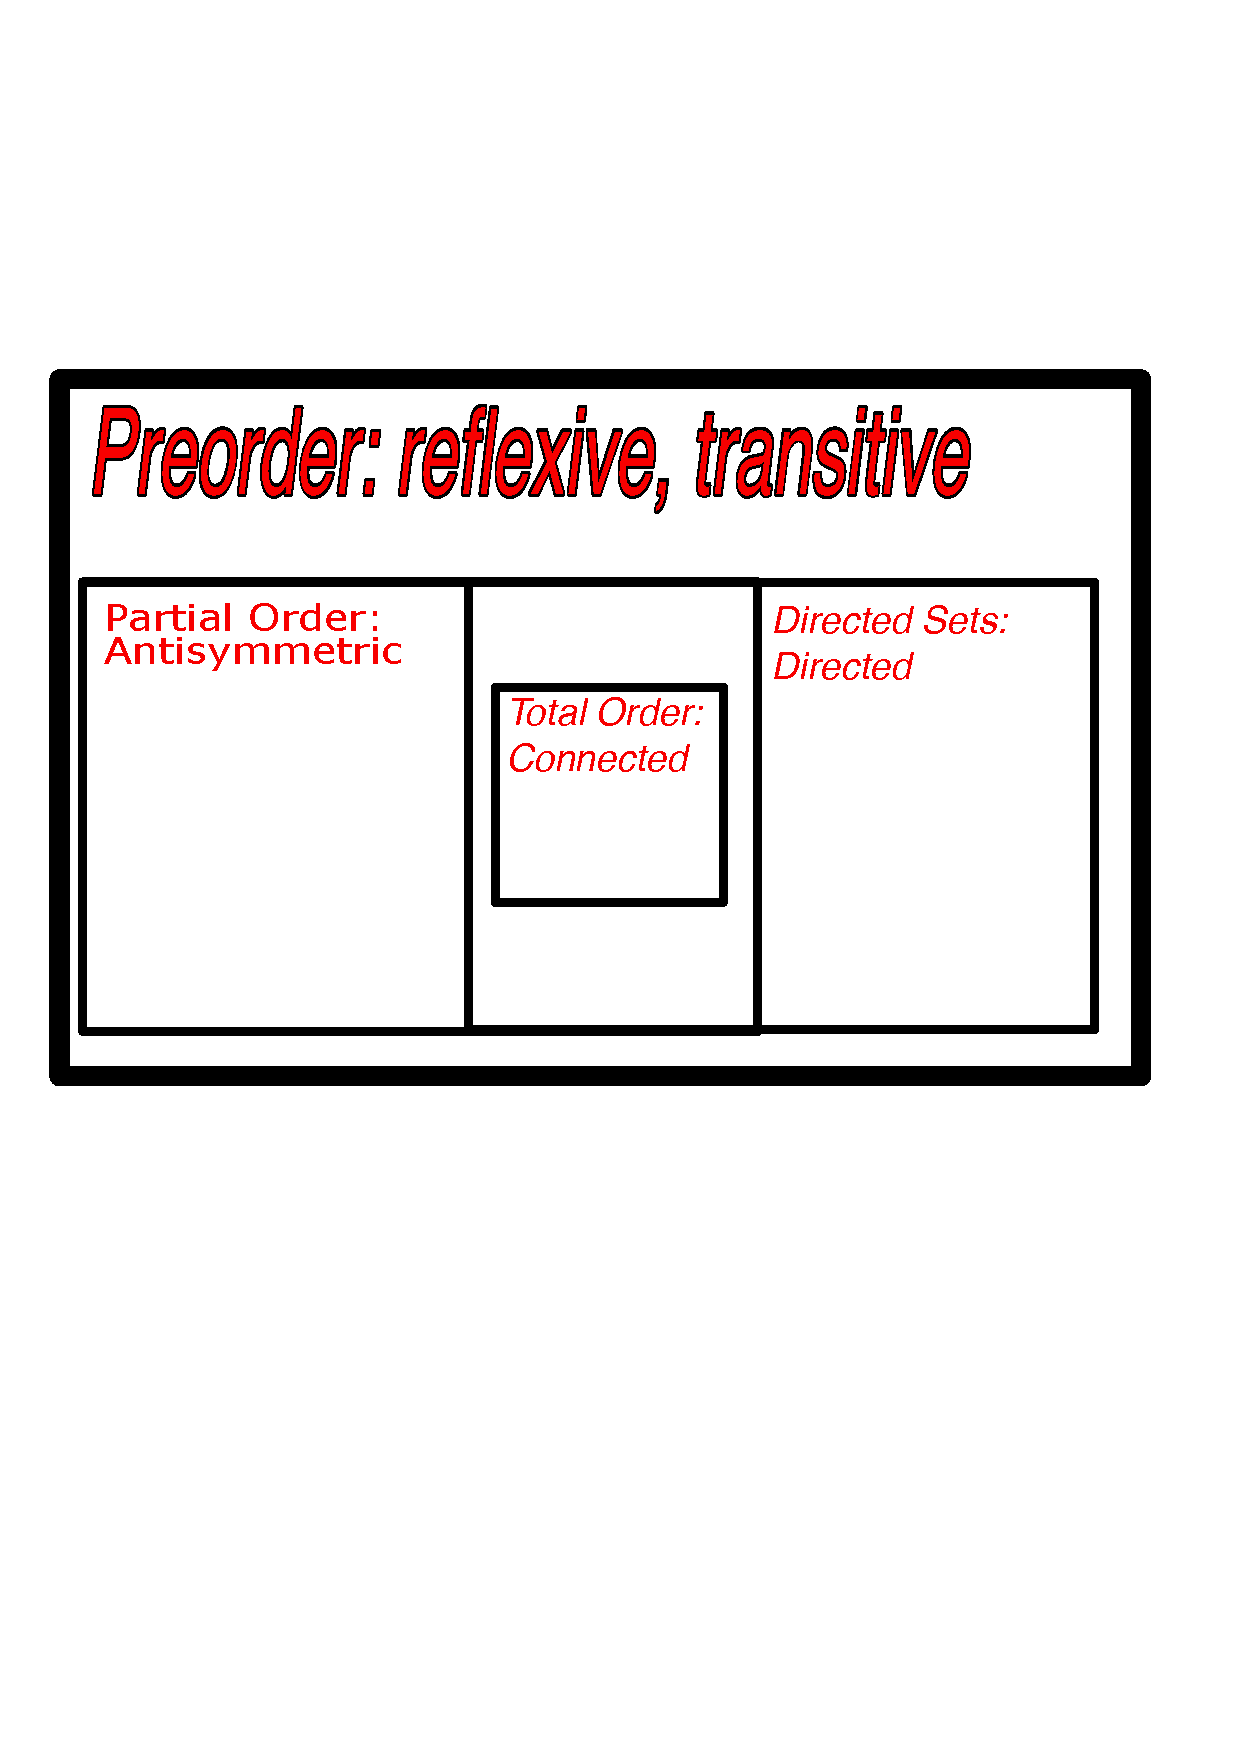
\includegraphics[height=10cm,width=10cm]{drawing.pdf}
\end{mdframed}
\begin{definition}
\label{1.1.9}
\textbf{(Definition of Cofinal)} Given a directed set $\mathcal{D}$, a subset $\mathcal{D}'\subseteq \mathcal{D}$ is called cofinal if 
\begin{align*}
\forall d \in \mathcal{D},\exists e\in \mathcal{D}', d\leq e 
\end{align*}
\end{definition}
\begin{theorem}
\label{1.1.10}
\textbf{(Cofinal Subset is a Directed Set with Original Order)} Given a directed set $\mathcal{D}$
 \begin{align*}
 \mathcal{D}'\subseteq \mathcal{D}\text{ is cofinal }\implies \mathcal{D}'\text{ is a directed set }
 \end{align*}
\end{theorem}
\begin{proof}
Arbitrarily pick two $a,b \in \mathcal{D}'$. Because $\mathcal{D}\ni a,b$ is directed, we know 
\begin{align*}
\exists c \in \mathcal{D}, a\leq c \text{ and } b\leq c
\end{align*}
Then because $\mathcal{D}'$ is cofinal in $\mathcal{D}$, we know 
\begin{align*}
\exists d \in \mathcal{D}', c\leq d
\end{align*}
Then because transitivity of directed set, our proof is finished, as we have found an element $d$ in $\mathcal{D}'$ that is greater than the arbitrary picked elements $a,b \in \mathcal{D}'$. 
\end{proof}
\section{Net}
\begin{definition}
\label{1.2.1}
  \textbf{(Subnet)} Given a net $w:\mathcal{D}\rightarrow X$ and $v:\mathcal{E}\rightarrow X$ and a function $h:\mathcal{E}\rightarrow \mathcal{D}$ we say $v$ is a subnet of $w$ if  
\begin{align*}
\begin{cases}
\forall e,e' \in \mathcal{E}, e\leq e' \implies h(e)\leq h(e')\text{(monotone)}\\
h[E]\text{ is cofinal in $\mathcal{D}$ }\\
v=w\circ h
\end{cases}
\end{align*}
\end{definition}
\begin{definition}
\textbf{(Net convergence)} We say the net $w:\mathcal{D}\rightarrow X$ converge to $x$, $w \to x$ if 
\begin{align*}

\end{align*}
\end{definition}
\begin{theorem}
\textbf{($w \to x \implies v \to x$)} Suppose $v$ is a subnet of $w$, we have 
 \begin{align*}
w \to x \implies v \to x
\end{align*}
\end{theorem}
\begin{proof}

\end{proof}
\begin{theorem}
\textbf{()}
\end{theorem}
\begin{definition}
\textbf{()}
\end{definition}
\chapter{Metric Space}
\section{}      
\chapter{Calculus}
\section{Examples for uniform convergence} 
\begin{theorem}
\textbf{(Test Example)} The sequence 
\begin{align*}
f_n(x)=\frac{x^2}{x^2+(1-nx)^2}\text{ is not equicontinuous on $[0,1]$ }
\end{align*}
\end{theorem}
\begin{proof}
Notice that 
\begin{align*}
f_n(\frac{1}{n})=1\text{ and }f_n(0)=0
\end{align*}
Then for all $\delta$, we see that if $n$ is large enough 
 \begin{align*}
\text{ then }\abso{\frac{1}{n}-0}<\delta \text{ and }\abso{f_n(\frac{1}{n})-f_n(0)}=1
\end{align*}
\end{proof}
\begin{theorem}
\textbf{(Test Example)} Prove 
\begin{align*}
\frac{x}{1+nx^2}\text{ uniformly converge on $\R$ }
\end{align*}
\end{theorem}
\begin{proof}
It is clear that $\frac{x}{1+nx^2}$ pointwise converge to $0$. Because $\frac{x}{1+nx^2}$ is an odd function, fixing $\epsilon $, we only wish to find $N$ such that 
\begin{align*}
\forall x>0, \forall n>N, \frac{x}{1+nx^2}<\epsilon 
\end{align*}
Observe 
\begin{align*}
  \frac{x}{1+nx^2}<\epsilon &\iff x<\epsilon (1+nx^2)\\
  &\iff \frac{x-\epsilon }{\epsilon x^2}<n
\end{align*}
Notice that $\frac{x-\epsilon }{\epsilon x^2}$ is bounded since it is continuous and converge to $0$ as  $x \to \infty$. 
\end{proof}
\section{Test Example}
\begin{theorem}
\textbf{(Cauchy-Schwarz Inequality for Integral)} Let $\mathscr{R}\Big([a,b] \Big)$ be the space of Riemann-Integrable functions on $[a,b]$. It is clear that $\mathscr{R}\Big([a,b] \Big)$ is a vector space over $\R$.  Define $\langle \cdot , \cdot \rangle $ on $\mathscr{R}\Big([a,b] \Big)$ by 
\begin{align*}
\langle f,g\rangle = \int_a^b f(x)g(x)dx
\end{align*}
It is easy to show  
\begin{enumerate}[label=(\alph*)]
  \item $ \forall f \in \mathscr{R}\Big([a,b] \Big), \langle f,f\rangle \geq 0 $ (non-negativity) 
  \item $\forall f,g \in \mathscr{R}\Big([a,b] \Big),\langle f,g\rangle =\langle g,f\rangle $ (Symmetry)
  \item $\forall f,g,h \in \mathscr{R}\Big([a,b] \Big),\forall c \in \R, \langle cf+g,h\rangle =c\langle f,h\rangle +\langle g,h \rangle $ (Linearity in first argument)
\end{enumerate}
This make $\langle \cdot,\cdot\rangle $ a \textbf{positive semi-definite Hermitian form}. We shall prove Cauchy-Schwarz Inequality hold for positive semi-definite Hermitian form. That is, we shall prove 
\begin{align*}
\forall f ,g \in \mathscr{R}\Big([a,b] \Big),\langle f,g \rangle \leq \norm{f}\cdot \norm{g}
\end{align*}
\end{theorem}
\begin{proof}
\end{proof}
\begin{theorem}
\textbf{(Application)} Given $f \in \mathscr{R}\Big([a,b] \Big)$ such that 
\begin{enumerate}[label=(\alph*)]
  \item $f(a)=0=f(b)$ 
  \item $\int_a^b f^2 (x)dx =1$ 
  \item $f$ is continuously differentiable on  $(a,b)$
  \item $f' \in \mathscr{R}\Big([a,b] \Big)$
\end{enumerate}
We have 
\begin{align*}
\int_a^b xf(x)f'(x)=\frac{-1}{2}
\end{align*}
and have 
\begin{align*}
\int_a^b \big(f'(x) \big)^2 dx \cdot \int_a^b \big(xf(x) \big)^2 dx>\frac{1}{4}
\end{align*}


\end{theorem}
\begin{proof}
Notice that 
\begin{align*}
  \frac{d}{dx} xf^2(x)=f^2(x)+2xf(x)f'(x)
\end{align*}
Then by Integral by Part (We have to check $\big(xf^2(x) \big)'(t)=f^2(t)+2tf(t)f'(t)$ for all $t \in (a,b)$, and we have to check $xf^2(x)$ is continuous on $[a,b]$), we have 
\begin{align*}
1=\int_a^b f^2(x)dx=xf^2(x)\Big|_a^b - \int_a^b 2xf(x)f'(x)dx
\end{align*}
Then because $f(b)=f(a)=0$, we see 
\begin{align*}
2 \int_a^b xf(x)f'(x)dx=-1 
\end{align*}
We wish to show 
\begin{align*}
\norm{f'}^2 \cdot \norm{x f(x)}^2> \frac{1}{4}= \Big( \langle f',xf(x)\rangle \Big)^2
\end{align*}
It is clear that $\geq $ is valid from Cauchy-Schwarz Inequality. We have to prove $\neq $. In other words, we have to prove 
\begin{align*}
f'\text{ and }xf(x)\text{ are linearly independent }
\end{align*}
\As{$f'$ and $xf(x)$ are linearly dependent}. Then 
 \begin{align*}
\exists c\inr, \forall x\in [a,b], f'(x)=cxf(x)
\end{align*}
The solution for this first order linear homogeneous ODE is 
\begin{align*}
f(x)=Ae^{\frac{cx^2}{2}} \text{ where $A\inr$ depends on $f(a)$ and $f(b)$}
\end{align*}
Then because $f(a)=f(b)=0$, we see $A=0$. Then  $\int_a^b f^2(x)dx=0\tCaC$
\end{proof}
\begin{theorem}
\textbf{(Example)} Given $G,g,\alpha :[a,b]\rightarrow \R$, suppose
\begin{enumerate}[label=(\alph*)]
  \item $G'(x)=g(x)$ for all $x \in (a,b)$ ($G$ is differentiable  on  $(a,b)$)
  \item $G$ is continuous on  $[a,b]$
  \item $\alpha $ increase on $[a,b]$
  \item $g$ is properly Riemann-Integrable on  $[a,b]$
\end{enumerate}
Prove 
\begin{align*}
\int_a^b \alpha (x)g(x)dx= \alpha G\Big|_a^b - \int_a^b G(x)d\alpha  
\end{align*}
\end{theorem}
\begin{proof}

\end{proof}
\section{Dini's Theroem}
\begin{theorem}
\textbf{(Dini's Theorem)} Given a topological space $X$ and a sequence of functions  $f_n:X\rightarrow \R$, suppose
\begin{enumerate}[label=(\alph*)]
  \item $X$ is compact
  \item $f_n$ is continuous  
  \item $f_n\to f$ pointwise  
  \item $f$ is continuous  
  \item $f_n(x)\leq f_{n+1}(x)$ for all $x \in X$
\end{enumerate}
Then 
\begin{align*}
f_n \to f \text{ uniformly }
\end{align*}
\end{theorem}
\begin{proof}
  Define $g_n:X\rightarrow \R$ 
\begin{align*}
g_n=f-f_n
\end{align*}
We reduce the problem into 
\begin{align*}
\vi{\text{ proving }g_n \to 0\text{ uniformly }}
\end{align*}
Notice that we have the property 
\begin{enumerate}[label=(\alph*)]
  \item $g_n(x)\geq g_{n+1}(x)$ for all $x \in X$ 
  \item $g_n$ is continuous 
   \item $g_n \to 0$ pointwise
\end{enumerate}
Fix $\epsilon $. We wish 
\begin{align*}
\vi{\text{ to find $N$ such that }\forall n>N, \forall x \in X,  g_n(x)<\epsilon }
\end{align*}
Define $E_n \subseteq X$ by 
\begin{align*}
E_n= \set{x \in X: g_n(x)<\epsilon }
\end{align*}
Because $g_n$ is continuous and  $E_n=g_n^{-1}\Big[(-\infty,\epsilon ) \Big]$, we know 
\begin{align*}
E_n\text{ is open for all $n \inn$ }
\end{align*}
We first prove 
\begin{align*}
\blue{\set{E_n}_{n\inn}\text{ is an open cover of $X$ }}
\end{align*}
Fix $y \in X$. We wish 
\begin{align*}
\blue{\text{ to find $n$ such that }y \in E_n}
\end{align*}
Because $g_n(y)\to 0$, this is clear. $\bdone$\\

We now prove 
\begin{align*}
\olive{\set{E_n}_{n\inn}\text{ is ascending }}
\end{align*}
Fix $n \inn$. We wish 
\begin{align*}
\olive{\text{ to prove }E_n\subseteq E_{n+1}}
\end{align*}
Because $g_n(x)\geq g_{n+1}(x)$ for all $x \in X$ and $E_n=g_{n}^{-1}\Big[(-\infty,\epsilon ) \Big]$ by definition, we see 
\begin{align*}
y \in E_n \implies g_{n+1}(y)<g_n(y)<\epsilon \implies y \in E_{n+1}\odone
\end{align*}
Now, because $X$ is compact and $\set{E_n}_{n\inn}$ is an open cover of $X$, we know  
\begin{align}
\label{Dimi1}
\text{ there exists $N$ such that  $X \subseteq \bigcup_{k=1}^N E_k= E_N$ }
\end{align}
It is clear such $N$ works.  $\vdone$
\end{proof}
\section{Fourier Stuff}
\begin{mdframed}
Suppose $f$ is a complex valued function Riemann-Integrable on  $[-\pi,\pi]$, and 
\begin{align*}
  c_n&\triangleq \frac{1}{2\pi}\int_{-\pi}^{\pi} f(x)e^{-inx}dx\\
s_N(x)&\triangleq \sum_{n=-N}^{N} c_ne^{inx} 
\end{align*}
Show 
\begin{align*}
\frac{1}{2\pi}\int_{-\pi}^{\pi} \abso{s_N(x)}^2dx=\sum_{n=-N}^{N}\abso{c_n}^2
\end{align*}
\end{mdframed}



\chapter{Multi-Variable Calculus}
\section{}
\chapter{HW}
\section{HW1}
\begin{question}{}{}
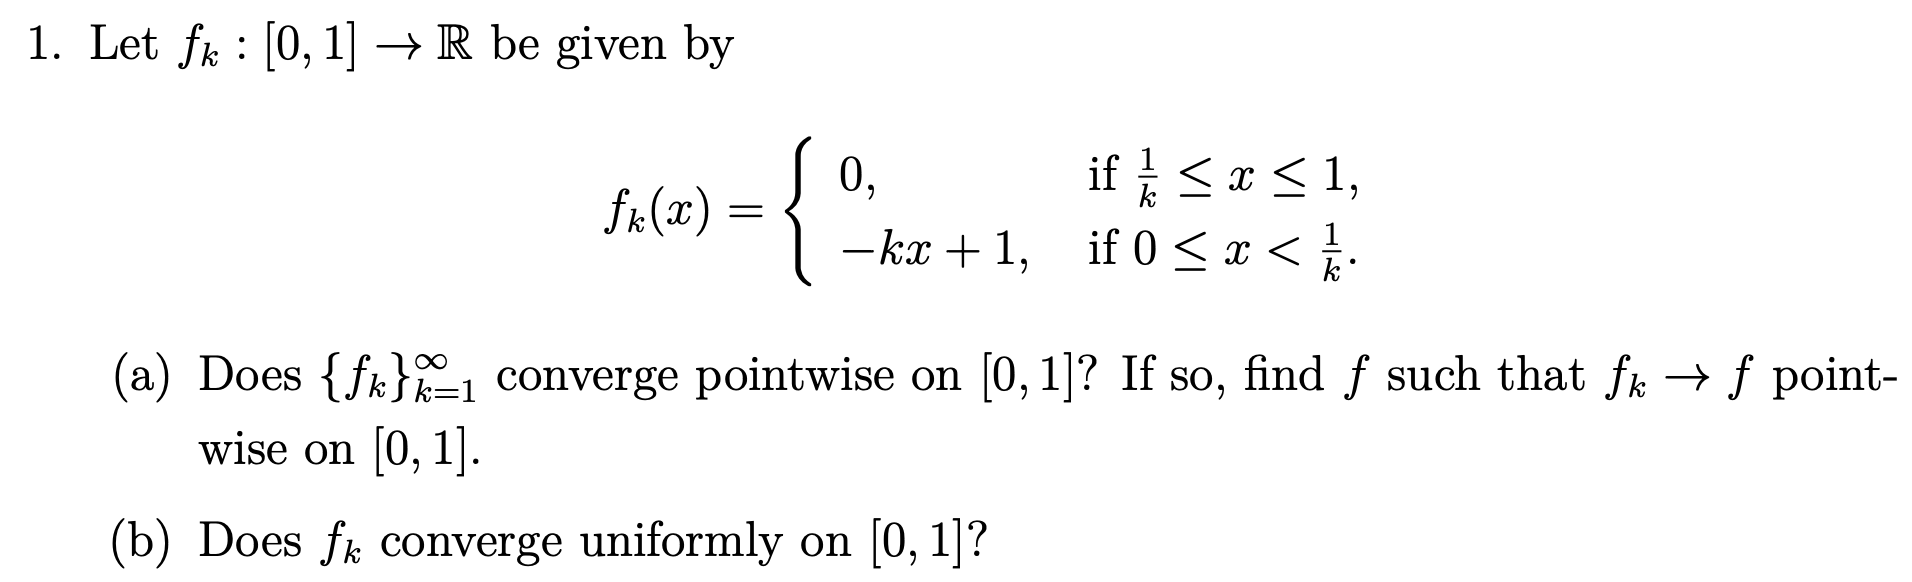
\includegraphics[height=5cm,width=18cm]{HW1.7}
\end{question}
\begin{proof}
\textbf{(a)} 
We claim 
\begin{align*}
\vi{f_k \to f\text{ pointwise  on $[0,1]$ where }f(x)=\begin{cases}
    0& \text{ if $x\in (0,1]$ } \\
    1& \text{ if $x=0$ }
\end{cases}}
\end{align*}
Because $\forall k\inn, f_k(0)=1$, it is clear $f_k(0)\to f(0)$. Now, let $x \in (0,1]$. We reduce our problem into proving 
\begin{align*}
\vi{f_k(x)\to 0\text{ as $k \to \infty$ }}
\end{align*}
By definition, we have 
\begin{align*}
\forall n>\frac{1}{x}, f_n(x)=0\vdone
\end{align*}
Above is true since $n>\frac{1}{x}\implies \frac{1}{n}<x$. 

\textbf{b}
No. It is easy to show that $f_k$ are all continuous and that $f$ is discontinuous at $0$. This let us deduce that the convergence is not uniform, since if it is, the function $f$ should have been continuous. 
\end{proof}
\begin{question}{}{}
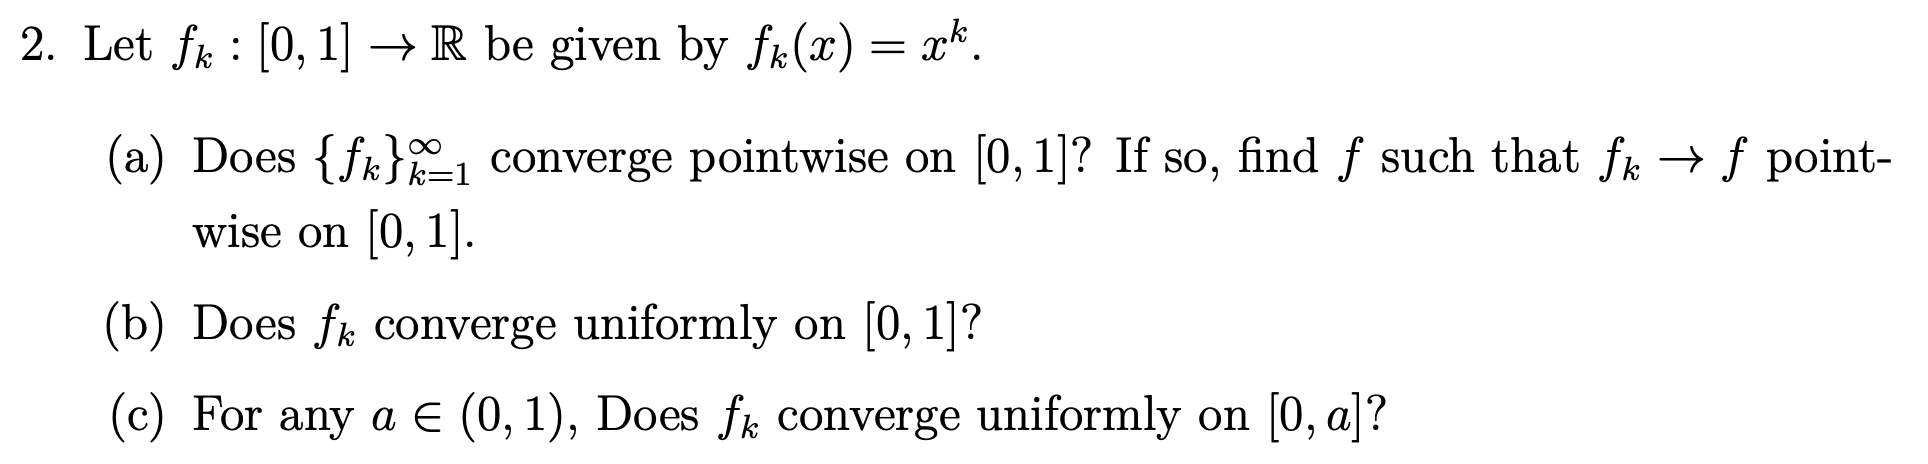
\includegraphics[height=5cm,width=18cm]{HW1.6}
\end{question}
\begin{proof}
\textbf{(a)} We claim 
\begin{align*}
\vi{f_k\to f\text{ pointwise on $[0,1]$ where }f(x)=\begin{cases}
  1& \text{ if $x=1$ }\\
  0& \text{ if $x\in [0,1)$ }
\end{cases}}
\end{align*}
Because $f_k(1)=1$ for all $k\inn$, it is clear $f_k(1)\to f(1)$. Now, let $x \in (0,1]$. We reduce our problem into proving 
\begin{align*}
\vi{f_k(x)\to 0\text{ as $k \to \infty$ }}
\end{align*}
Fix $\epsilon $. We wish  
\begin{align*}
\vi{\text{ to find $N$ such that }\forall n>N, f_n(x)< \epsilon }
\end{align*}
We claim 
\begin{align*}
  \vi{N>\log_x \epsilon\text{ works }}
\end{align*}
Fix $n>N$. Because $x<1$,  we see 
 \begin{align*}
f_n(x)=x^n<x^N<\epsilon \vdone
\end{align*}
\textbf{b}
No. It is easy to show that $f_k$ are all continuous and that $f$ is discontinuous at $1$. This let us deduce that the convergence is not uniform, since if it is, the function $f$ should have been continuous.\\

\textbf{(c)} Yes. Fix $\epsilon $ and $a \in (0,1)$. We wish to 
\begin{align*}
\vi{\text{ find $N$ such that }\forall n>N,\forall x \in [0,a], f_n(x)\leq \epsilon }
\end{align*}
We claim 
\begin{align*}
\vi{N>\log_a \epsilon \text{ works }}
\end{align*}
Observe 
\begin{align*}
\forall n >N, \forall  x\in [0,a], f_n(x)=x^n \leq a^n \leq a^N <\epsilon vdon
\end{align*}

\end{proof}
\begin{question}{}{}
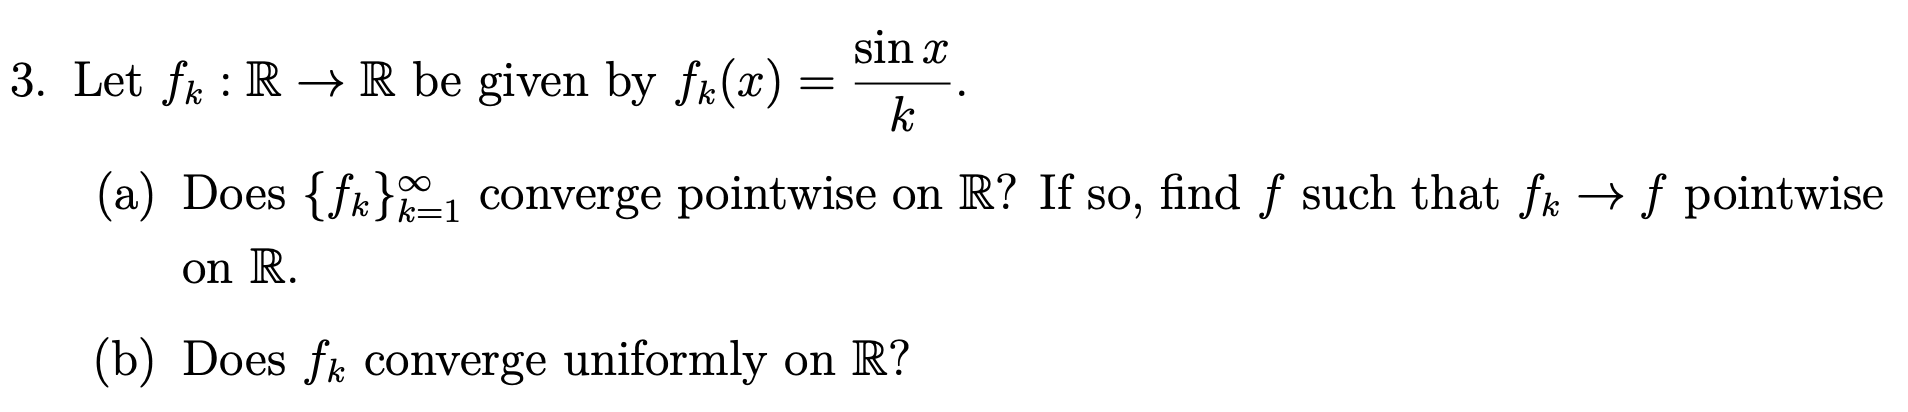
\includegraphics[height=5cm,width=18cm]{HW1.5}
\end{question}
\begin{proof}
We show 
\begin{align*}
\vi{f_k\to 0\text{ uniformly }}
\end{align*}
Remark: Notice that the $0$ above is the function that map all reals to $0$.\\

Fix $\epsilon $. 
\begin{align*}
\vi{\text{ find $N$ such that }\forall n>N, \norm{f_n-0}_\infty \leq \epsilon }
\end{align*}
We claim 
\begin{align*}
  \vi{N>\frac{1}{\epsilon }\text{ works }}
\end{align*}
Using the fact $\abso{\sin x}\leq 1$ for all $x \inr$, we can deduce 
\begin{align*}
\forall n>N, \forall x\inr, \abso{f_n(x)}=\abso{\frac{\sin x}{n}}\leq \frac{1}{n}<\frac{1}{N}< \epsilon 
\end{align*}
This then implies $\norm{f_n-0}_{\infty}\leq \epsilon\vdone $.\\

Remark: Notice that it is of course possible that $\norm{f_N}_\infty=\epsilon $. This is why you shouldn't always set the goal by proving strict inequality when proving convergence. That maybe "technically cool" if you catch my drift, but it is just unnecessary and stupid. 
\end{proof}
\begin{question}{}{}
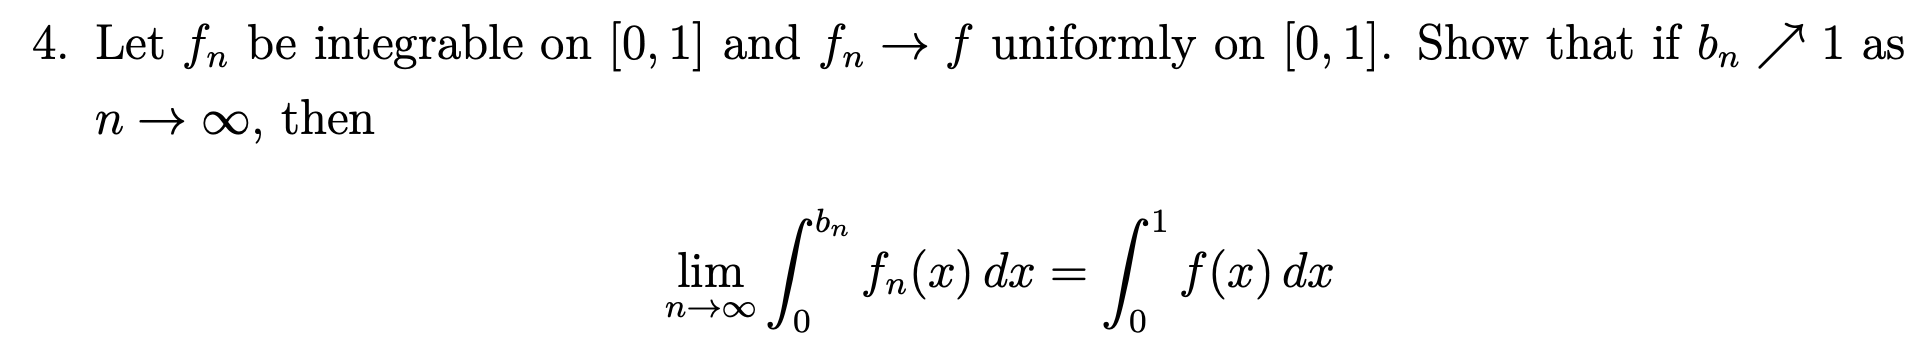
\includegraphics[height=5cm,width=18cm]{HW1.4}
\end{question}
\begin{proof}
Because $f_n$ is Riemann-integrable on $(0,1)$ and $f_n\to f$ uniformly on $(0,1)$. We know $f$ is Riemann-integrable on  $(0,1)$ and  
\begin{align*}
\int_0^1 f_ndx \to \int_0^1 f(x)dx\text{ as }n\to \infty
\end{align*}
Then 
\begin{align*}
\lim_{n\to \infty}\int_0^{b_n}f_ndx=\lim_{n\to \infty}\Big(\int_0^1 f_ndx-\int_{b_n}^1 f_ndx \Big)=\int_0^1 fdx-\lim_{n\to \infty}\int_{b_n}^1 f_ndx
\end{align*}
This let us reduce the problem into proving 
\begin{align*}
\vi{\int_{b_n}^1 f_ndx \to 0\text{ as }n \to \infty}
\end{align*}
Fix $\epsilon $. We wish 
\begin{align*}
\vi{\text{ to find $N$ such that }\forall n>N, \abso{\int_{b_n}^1 f_ndx}\leq  \epsilon }
\end{align*}
Because each $f_n:[0,1]\rightarrow \R$ is bounded  ($f_n$ is integrable), and $f_n \to f$ uniformly. We know $f_n$ are uniformly bounded (This will be \textit{fully} justified in the proof for  Question 7). Then, we know there exists $M$ such that 
\begin{align*}
M> \sup_n (\sup_{[0,1]} \abso{f_n}) 
\end{align*}
Because $b_n \nearrow 1$. We know 
\begin{align*}
\exists N, \forall n>N, \abso{b_n-1} < \frac{\epsilon}{M}
\end{align*}
We claim 
\begin{align*}
\vi{\text{ such $N$ works }}
\end{align*}
Let $n>N$. See 
 \begin{align*}
   \abso{\int_{b_n}^1 f_ndx}&\leq \int_{b_n}^1 \abso{f_n}dx\\
   &\leq \int_{1-\frac{\epsilon}{M}}^1 \abso{f_n}dx\\
   &\leq \int_{1-\frac{\epsilon}{M}}^1 Mdx=\epsilon \vdone
\end{align*}
\end{proof}
\begin{lemma}
\label{pouc}
\textbf{(product of uniformly convergent sequence is uniformly convergent on bounded domain)} Given 
\begin{enumerate}[label=(\alph*)]
   \item $f_n\to f\text{ and }g_n\to g$ uniformly on $I$
  \item $f,g$ are bounded on $I$ 
\end{enumerate}
Then 
\begin{align*}
f_ng_n \to fg\text{ on }I
\end{align*}
\end{lemma}
\begin{proof}
Observe 
\begin{align*}
  \abso{(f_ng_n)(x)-(fg)(x)}&=\abso{\big((f_n-f)g_n \big)(x)+\big(f(g_n-g) \big)(x)}\\
  &\leq \abso{(f_n-f)(x)}\cdot \abso{g_n(x)}+\abso{f(x)}\cdot \abso{(g_n-g)(x)}
\end{align*}
Notice that there exists $M$ globally greater than both $\abso{g_n}$ and $\abso{f}$, and that $(f_n-f)(x)$ and $(g_n-g)(x)$ both uniformly converge to $0$ and we are done.
\end{proof}
\begin{question}{}{}
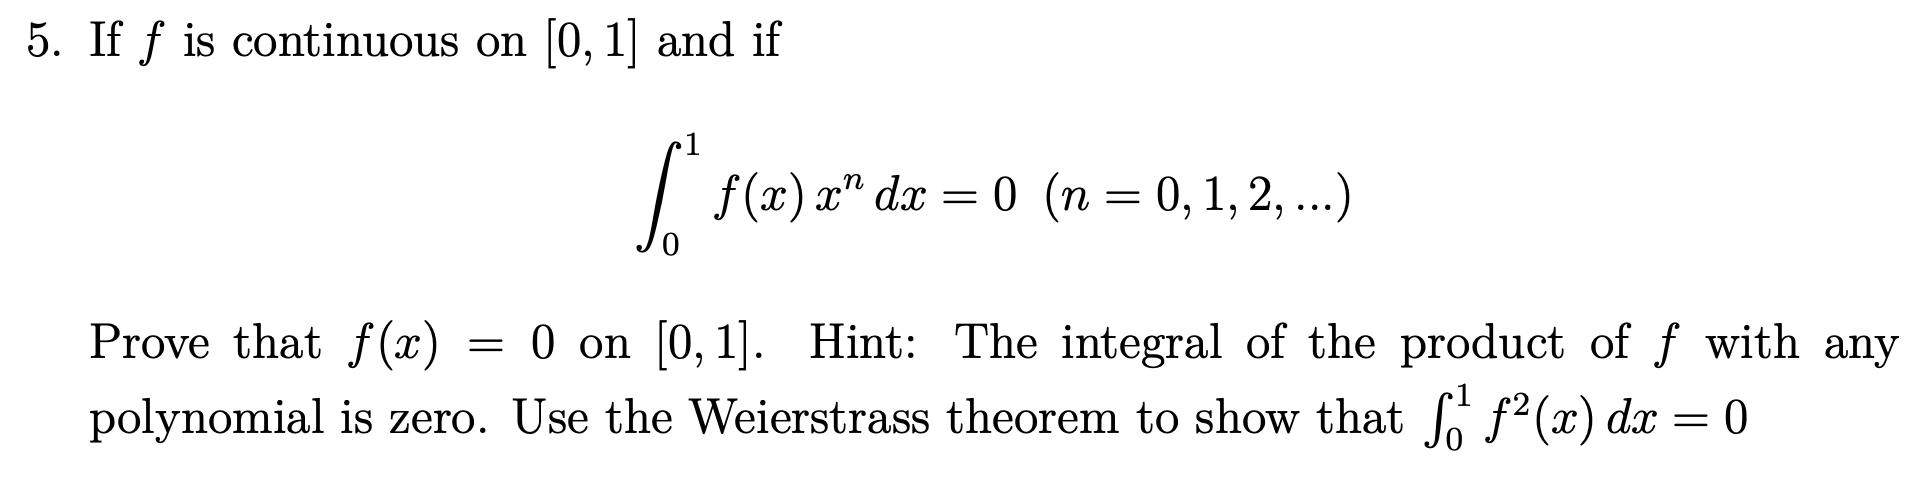
\includegraphics[height=5cm,width=18cm]{HW1.3}
\end{question}
\begin{proof}
By Stone-Weierstrass Theorem, there exists a sequence of polynomial $P_k \to f$ uniformly. Because each polynomial is an finite linear combination of $x^n\hspace{0.5cm}(n=0,1,2,\dots)$, from premise we can deduce
\begin{align*}
\int_0^1 f P_kdx=0\text{ for all $k\inn$ }
\end{align*}
Because $f$ is continuous on the compact domain $[0,1]$ and $P_n \to f$. It is easy to see that $f$ and  $P_n$ satisfy the hypothesis of \myref{Lemma}{pouc}. Then, we see 
\begin{align*}
fP_n \to f^2\text{ uniformly }
\end{align*}
This then let us deduce 
\begin{align*}
\int_0^1 f^2 dx=0
\end{align*}
\As{$f(x)\neq 0$ for some $x \in [0,1]$}, in the aiming for a contradiction. Because $f^2$ is continuous at $x$ ($\because$  $f$ is continuous at $x$). We know there exists  $\delta$ such that 
\begin{align*}
\inf_{[x-\delta,x+\delta]}f^2=\alpha >0
\end{align*}
for some appropriate $\alpha $, says, $\alpha =\frac{f^2(x)}{2}$.\\

Now, because $f^2\geq 0$, we have 
\begin{align*}
  \int_0^1 f^2dt\geq \int_{x-\delta}^{x+\delta}f^2dt\geq 2\delta \alpha >0 \tCaC\text{ to }\int_0^1 f^2dt=0
\end{align*}
\end{proof}
\begin{question}{}{}
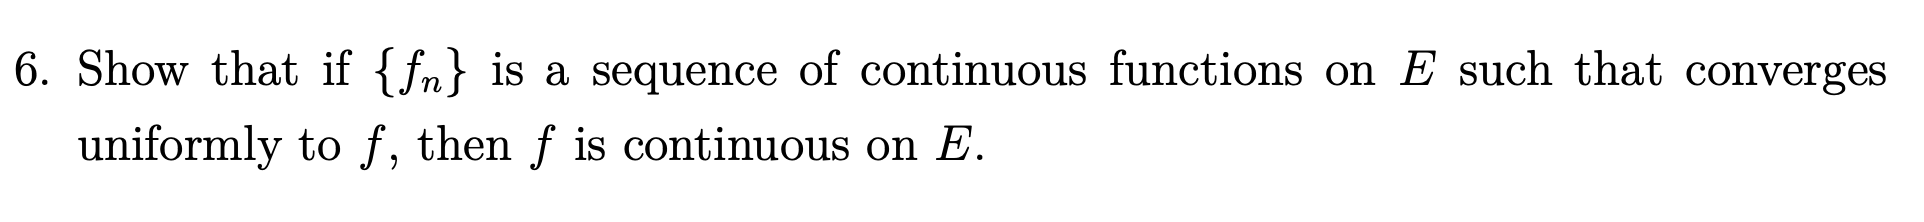
\includegraphics[height=3cm,width=18cm]{HW1.2}
\end{question}
\begin{proof}
Click the following hyperlink
(\myref{Theorem}{ULT})
\end{proof}
\begin{question}{}{}

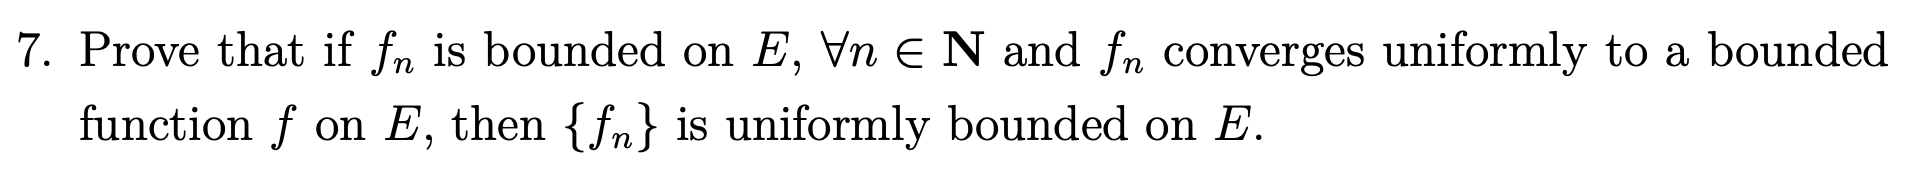
\includegraphics[height=3cm,width=18cm]{HW1.1}
\end{question}
\begin{proof}
We first prove 
\begin{align*}
\vi{f\text{ is bounded }}
\end{align*}
\As{$f$ is not bounded}. Let $p \in E$, we know there exists sequence  $x_n \subseteq E$ such that  $d(f(x_n),p) \to \infty$. Now, for arbitrary $k \inn$, we see
\begin{align*}
d(f(x_n),p)\leq d(f_k(x_n),f(x_n))+d(f_k(x_n),p)
\end{align*}
Then because $f_k(x_n) \to f(x_n)$ uniformly, this give us 
\begin{align*}
d(f_k(x_n),p)\geq d(f(x_n,p))-d(f_k(x_n),f(x_n))\to \infty
\end{align*}
This implies $f_k$ is unbounded \CaC. $\vdone$\\

We now prove 
\begin{align*}
\blue{f_n\text{ is uniformly bounded }}
\end{align*}
Let $p \in E$ and $M \inr^+$ satisfy 
\begin{align*}
f[E]\subseteq B_M(p)
\end{align*}
Because $\norm{f_n-f}_\infty \to 0$, we know there exists $L\inr^+$ such that $\norm{f_n-f}_\infty <L$ for all $n\inn$. We claim 
\begin{align*}
\blue{\bigcup_{n\inn}f[E]\subseteq B_{M+L}(p)}
\end{align*}
Fix $n \inn$ and $x \in E$. We wish to show 
\begin{align*}
\blue{d(f_n(x),p)<M+L}
\end{align*}
Observe 
\begin{align*}
d(f_n(x),p)\leq d(f_n(x),f(x))+d(f(x),p)< L+M \bdone
\end{align*}
\end{proof}
\begin{question}{}{}
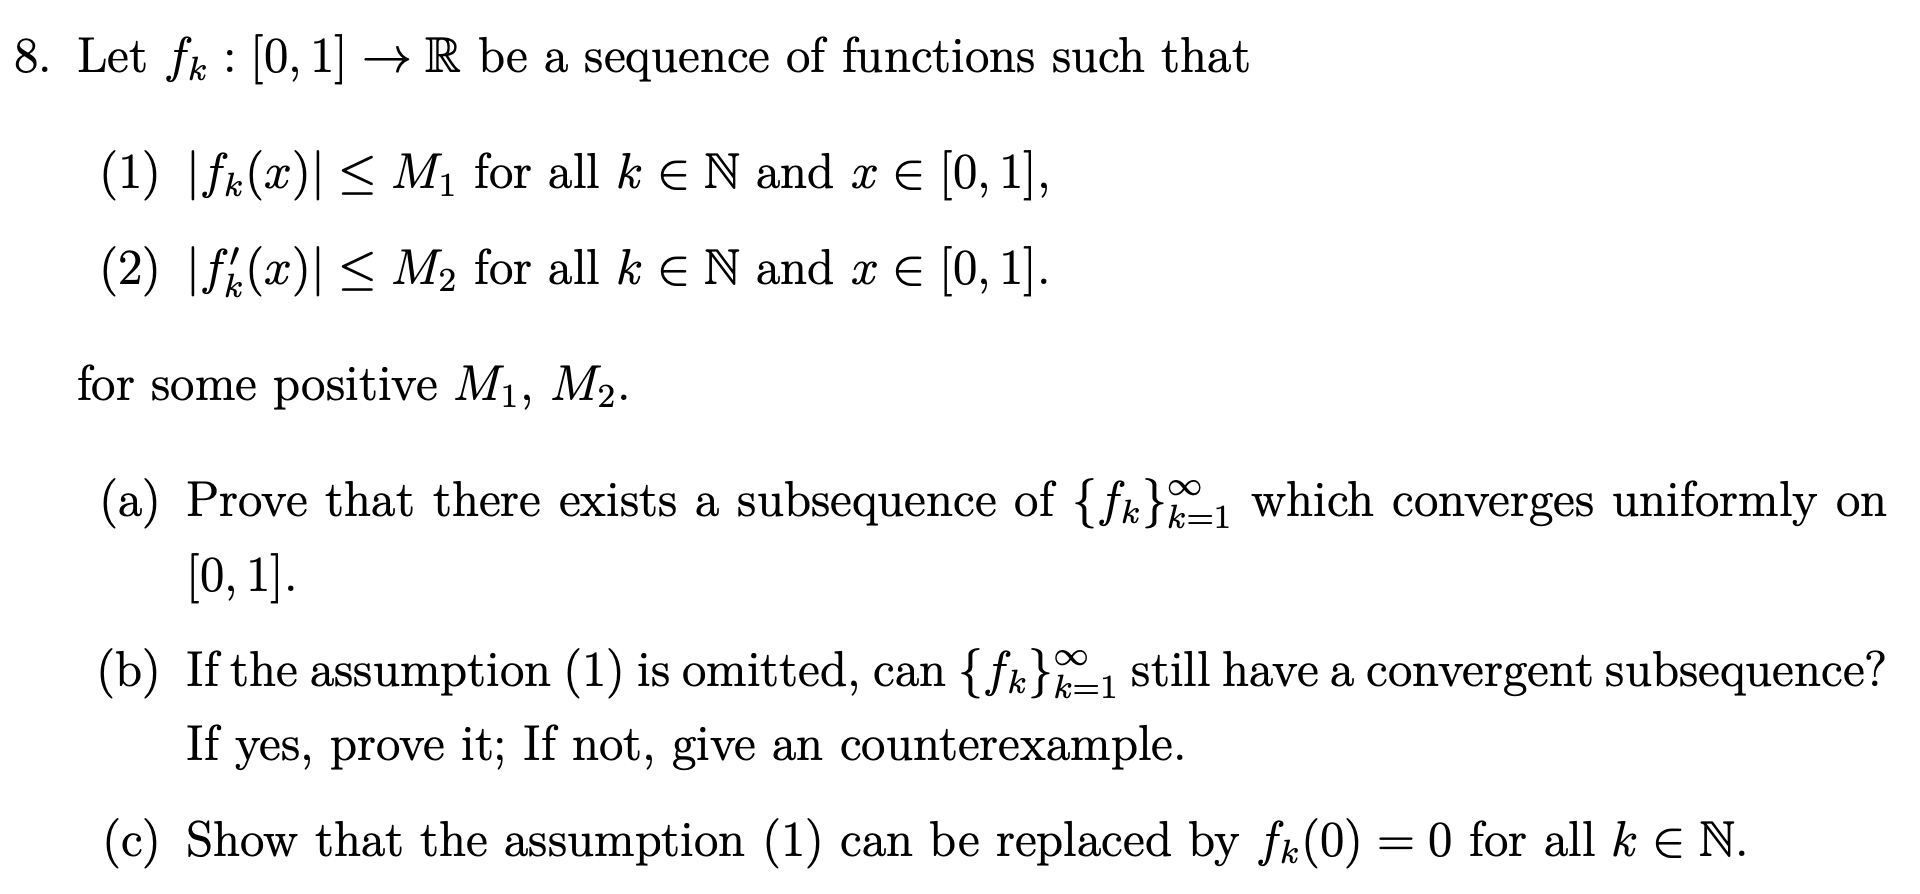
\includegraphics[height=9cm,width=18cm]{HW1.8}
\end{question}
\begin{proof}
\textbf{(a)} The assumption (1) implies $f_k$ is pointwise bounded.  We first show 
\begin{align*}
\vi{f_k\text{ are equicontinuous }}
\end{align*}
Fix $\epsilon $. We wish to find $\delta$ such that 
\begin{align*}
  \vi{\forall n \inn, \forall x,y \in [0,1], \abso{x-y}<\delta \implies \abso{f_n(x)-f_n(y)}\leq \epsilon }
\end{align*}
We claim 
\begin{align*}
\vi{\delta < \frac{\epsilon}{M_2}\text{ works }}
\end{align*}
Fix $n\inn$ and $x,y \in [0,1]$ such that $\abso{x-y}<\delta$. By Lagrange's MVT, we see 
\begin{align*}
\frac{\abso{f_k(x)-f_k(y)}}{\abso{x-y}}\leq M_2
\end{align*}
Then 
\begin{align*}
\abso{f_k(x)-f_k(y)}\leq M_2\cdot \abso{x-y}\leq  M_2\cdot \delta =\epsilon \vdone
\end{align*}
\textbf{(b)}. No. Consider $f_k(x)=x+k$. It is clear that $f_k(x)$ has no even pointwise convergent sequence, as for all $x_0$, the sequence  $f_k(x_0)$ diverge.\\

\textbf{(c)} 
Suppose we are given assumption (2). It suffice to show that 
\begin{align*}
  \vi{\forall k\inn,f_k(0)=0\implies \exists M_1\inr^+, \forall k\inn, \forall x\in [0,1],\abso{f_k(x)}\leq M_1}
\end{align*}
We claim 
\begin{align*}
\vi{M_1=M_2\text{ works }}
\end{align*}
Fix $k\inn$ and $x\in [0,1]$. By FTC and assumption two, we see 
\begin{align*}
\abso{f_k(x)}=\abso{\int_0^x f_k'dt}\leq  \int_0^x \abso{f_k'}dt\leq \int_0^1 \abso{f'_k}dt\leq \int_0^1 M_2dt=M_2=M_1\vdone
\end{align*}







\end{proof}

\section{Limit Interchange}
\begin{mdframed}
Given an arbitrary set $X$ and  a complete metric space  $(\overline{Y},d)$, in \myref{Section}{27CaB}, we have proved that the set of functions with the following properties 
\begin{enumerate}[label=(\alph*)]
  \item boundedness 
  \item unboundedness
\end{enumerate}
are respectively closed under uniform convergence. In next section (\myref{Section}{UCaCH}), we will prove that the following three properties 
\begin{enumerate}[label=(\alph*)]
  \item continuity
  \item uniform continuity
  \item $K$-Lipschitz continuity
\end{enumerate}
are again all closed under uniform convergence, where the proof for continuity is closed under uniform convergence use \myref{Theorem}{COLO} as a lemma.\\

Here, we prove 
\begin{enumerate}[label=(\alph*)]
  \item convergent of sequences 
\end{enumerate}
in, of course, complete metric space, is also closed under uniform convergence.\\


The reason we require the codomain $\overline{Y}$ of sequence to be complete is explained in the last paragraph of \myref{Section}{27CaB}. An example of such beautiful closure is lost if the codmain $(Y,d)$ is not complete is $Y=\R^*$ and  $a_{n,k}=\frac{1}{n}+\frac{1}{k}$. 
\end{mdframed}
\begin{theorem}
\label{COLO}
\textbf{(Change Order of Limit Operations: Part 1)} Given a double sequence $a_{n,k}$ whose codomain is $(Y,d)$. Suppose
\begin{enumerate}[label=(\alph*)]
  \item $a_{n,k}\to a_{\bullet,k}$ uniformly as $n\to \infty$ 
  \item $a_{n,k}\to A_n$ pointwise as  $k\to \infty$.
  \item $A_n \to A$ 
\end{enumerate}
Then we can deduce 
\begin{align*}
\lim_{k\to \infty}a_{\bullet,k}\text{ exists and }\lim_{k\to \infty}a_{\bullet,k}=A
\end{align*}
In other words, we can switch the order of limit operations
\begin{align*}
\lim_{k\to \infty}\lim_{n\to \infty}a_{n,k}=\lim_{n\to \infty}\lim_{k\to \infty}a_{n,k}
\end{align*}
\end{theorem}
\begin{proof}
We wish to prove 
\begin{align*}
\vi{a_{\bullet,k}\to A\text{ as }k\to \infty}
\end{align*}
Fix $\epsilon $. Because $a_{n,k}\to a_{\bullet,k}$ uniformly and $A_n\to A$ as $n\to \infty$, we know there exists $m$ such that 
 \begin{align}
  \label{K1}
d(A_m,A)<\frac{\epsilon}{3}\text{ and }\forall k\inn,d(a_{m,k},a_{\bullet,k})<\frac{\epsilon}{3}
\end{align}
Then because $a_{m,k}\to A_m$ as $k\to \infty$, we know there exists $K$ such that
\begin{align}
\label{K2}
\forall k>K, d(a_{m,k},A_m)<\frac{\epsilon}{3}
\end{align}
We now claim 
\begin{align*}
  \vi{\forall k>K, d(a_{\bullet,k},A)<\epsilon}
\end{align*}
The claim is true since by \myref{Equation}{K1} and \myref{Equation}{K2}, we have 
\begin{align*}
  \forall k>K, d(a_{\bullet,k},A)\leq d(a_{\bullet,k},a_{m,k})+d(a_{m,k},A_m)+d(A_m,A)<\epsilon \vdone
\end{align*}
\end{proof}
\begin{theorem}
\label{COLO2}
\textbf{(Change Order of Limit Operations: Part 2)} Given a double sequence $a_{n,k}$ whose codomain is $(Y,d)$. Suppose 

\begin{enumerate}[label=(\alph*)]
  \item $a_{n,k}\to a_{\bullet,k}$ uniformly as $n\to \infty$ 
  \item $a_{n,k}\to A_n$ pointwise as $k\to \infty$ 
  \item $a_{\bullet,k}\to A$ as $k\to \infty$
\end{enumerate}
Then we can deduce
\begin{align*}
A_n\text{ converge and  }A_n \to A
\end{align*}
\end{theorem}
\begin{proof}
Fix $\epsilon $. We wish to find $N$ such that 
 \begin{align*}
   \vi{\forall n>N, d(A_n,A)<\epsilon}
\end{align*}
Because  $a_{n,k}\to a_{\bullet,k}$ uniformly as $n \to \infty$, we can let $N$ satisfy 
\begin{align}
\label{K3}
\forall n>N,\forall k\inn, d(a_{n,k},a_{\bullet,k})<\frac{\epsilon}{3}
\end{align}
We claim 
\begin{align*}
\vi{\text{ such $N$ works }}
\end{align*}
Arbitrarily pick $n>N$. Because $a_{\bullet,k} \to A$, and because $a_{n,k} \to A_n$, we know there exists $j$ such that 
 \begin{align}
  \label{K4}
d(a_{\bullet,j},A)<\frac{\epsilon}{3}\text{ and }d(a_{n,j},A_n)<\frac{\epsilon}{3}
\end{align}
From \myref{Equation}{K3} and \myref{Equation}{K4}, we now have
\begin{align*}
d(A_n,A)\leq d(A_n,a_{n,j})+d(a_{n,j},a_{\bullet,j})+d(a_{\bullet,j},A)<\epsilon \vdone
\end{align*}
\end{proof}
\begin{mdframed}
In summary of \myref{Theorem}{COLO} and \myref{Theorem}{COLO2}, given a double sequence $a_{n,k}$ converging both side 
\begin{enumerate}[label=(\alph*)]
  \item $a_{n,k}\to a_{\bullet,k}$ pointwise as $n \to \infty$
  \item $a_{n,k}\to a_{n,\bullet}$ pointwise as $k\to \infty$
\end{enumerate}
As long as 
\begin{enumerate}[label=(\alph*)]
  \item one side of convergence is uniform 
  \item between two sequence $\set{a_{\bullet,k}}_{k\inn}$ and $\set{a_{n,\bullet}}_{n\inn}$, one of them converge, say, to $A$
\end{enumerate}
Then the other sequence also converge, and the limit is also $A$.\\

It is at this point, we shall introduce two other terminologies. Suppose $f_n$ is a sequence of functions from an arbitrary set  $X$ to a metric space  $Y$. We say $f_n$ is  \textbf{pointwise Cauchy} if for all fixed $x \in X$, the sequence $f_n(x)$ is Cauchy. We say $f_n$ is  \textbf{uniformly Cauchy} if for all $\epsilon $, there exists $N\inn$ such that 
\begin{align*}
\forall n,m>N, \forall x\in X, d\big(f_n(x),f_m(x) \big)<\epsilon 
\end{align*}
In last Section (\myref{Section}{27CaB}), we define the \textbf{uniform metric} $d_{\infty}$ on $X^Y$ by 
 \begin{align*}
d_{\infty}(f,g)=\sup_{x\in X}d\big(f(x),g(x) \big)
\end{align*}
and say that $f_n\to f$ uniformly if and only if $f_n\to f$ in $(X^Y,d_{\infty})$. Similar to this clear fact, we have 
\begin{align*}
f_n\text{ is uniformly Cauchy }\iff \text{ $f_n$ is Cauchy in  $(X^Y, d_\infty)$ }
\end{align*}
It should be very easy to verify that if $f_n$ uniformly converge, then $f_n$ is uniformly Cauchy, and just like sequences in metric space, the converse hold true if and only if the space $\big(X^Y,d_\infty \big)$ is complete. In \myref{Theorem}{Tsof}, we give a necessary and sufficient condition for $\big(X^Y,d_{\infty}\big)$ to be complete. 
\end{mdframed}
\begin{theorem}
\label{Tsof}
\textbf{(Space of functions $\big(X^Y,d_{\infty}\big)$ is Complete iff $Y$ is Complete)} Given an arbitrary set $X$ and a metric space  $(Y,d)$, we have 
\begin{align*}
\text{ the extended metric space $\big(X^Y,d_{\infty} \big)$ is complete }\iff Y\text{ is complete }
\end{align*}
\end{theorem}
\begin{proof}
$(\longleftarrow)$\\

Suppose $f_n$ is uniformly Cauchy. We wish 
\begin{align*}
  \vi{\text{ to construct a $f:X\rightarrow Y$ such that }f_n\to f\text{ uniformly }}
\end{align*}
Because $f_n$ is uniformly Cauchy, we know that for all $x \in X$, the sequence $f_n(x)$ is Cauchy in $(Y,d)$. Then because $Y$ is complete, we can define $f:X\rightarrow Y$ by 
 \begin{align*}
f(x)=\lim_{n\to \infty}f_n(x)
\end{align*}
We claim 
\begin{align*}
\vi{\text{ such $f$ works, i.e.  $f_n\to f$ uniformly }}
\end{align*}
Fix $\epsilon $. We wish 
\begin{align*}
  \vi{\text{ to find $N\inn$ such that for all $n>N$ and  $x \in X$ we have $d\big(f_n(x),f(x)\big)<\epsilon $ }}
\end{align*}
Because $f_n$ is uniformly Cauchy, we know there exists $N$ such that  
\begin{align}
\label{K5}
\forall n,m>N, \forall x\in X, d\big(f_n(x),f_m(x) \big)<\frac{\epsilon }{2}
\end{align}
We claim 
\begin{align*}
\vi{\text{ such $N$ works }}
\end{align*}
 \As{there exists $n>N\text{ and }x\in X$ such that  $d\big(f_n(x),f(x) \big)\geq \epsilon $}. Because $f_k(x)\to f(x)$ as $k\to \infty$, we know 
\begin{align}
  \label{K6}
\exists m \inn, d\big(f_m(x),f(x) \big)<\frac{\epsilon}{2}
\end{align}
Then from \myref{Equation}{K5} and \myref{Equation}{K6}, we can deduce 
\begin{align*}
\epsilon \leq d\big(f_n(x),f(x)\big)\leq  d\big(f(x),f_m(x)\big)  + d\big(f_n(x),f_m(x)\big)<\epsilon \tCaC \vdone
 \end{align*}
 $(\longrightarrow)$\\

Let $K$ be the set of constant functions  in $X^Y$. We first prove 
 \begin{align*}
\blue{K\text{ is closed }}
\end{align*}
Arbitrarily pick $f \in K^c$. We wish 
\begin{align*}
\blue{\text{ to find $\epsilon \inr^+$ such that $B_{\epsilon }(f) \in K^c$ }}
\end{align*}
Because $f$ is not a constant function, we know there exists $x_1,x_2 \in X$ such that 
\begin{align*}
d\big(f(x_1),f(x_2) \big)>0
\end{align*}
We claim that 
\begin{align*}
\blue{\epsilon=\frac{d\big(f(x_1),f(x_2) \big)}{3}\text{ works }}
\end{align*}
Arbitrarily pick $g \in B_\epsilon(f)$. We wish 
\begin{align*}
\blue{\text{ to show $g\in K^c$  }}
\end{align*}
Notice the triangle inequality 
\begin{align}
\label{K7}
3\epsilon =d\big(f(x_1),f(x_2) \big)\leq d\big(f(x_1),g(x_1) \big)+d\big(g(x_1),g(x_2) \big)+d\big(g(x_2),f(x_2) \big)
\end{align}
Also, because $g\in B_\epsilon (f)$, we have
\begin{align}
  \label{K8}
\forall x\in X, d\big(f(x),g(x) \big)<\epsilon 
\end{align}
Then by \myref{Equation}{K7} and \myref{Equation}{K8}, we see 
\begin{align*}
d\big(g(x_1),g(x_2) \big)> \epsilon 
\end{align*}
This then implies $g$ is not a constant function.  $\bdone$\\

Now, Because by premise $(X^Y,d_{\infty})$ is complete, and we have proved $K$ is closed in  $(X^Y,d_\infty)$, we know $K$ is complete. Then, we resolve the whole problem into proving 
\begin{align*}
\vi{Y \text{ is isometric to }K}
\end{align*}
Define $\sigma:Y \to K $ by 
\begin{align*}
y \mapsto \tilde{y}\text{ where }\forall x \in X, \tilde{y}(x)=y 
\end{align*}
It is easy to verify $\sigma$ is an isometry. $\vdone$
\end{proof}
\begin{corollary}
\label{SoB}
\textbf{(Space of Bounded functions $\big(B(X,Y),d_{\infty} \big)$ is Complete iff  $Y$ is Complete)} 
\begin{align*}
\big(B(X,Y),d_\infty \big)\text{ is complete }\iff  Y\text{ is complete }
\end{align*}
\end{corollary}
\begin{proof}
$(\longleftarrow)$\\

By \myref{Theorem}{Tsof}, the space $(X^Y, d_{\infty})$ is complete. Then because $B(X,Y)$ is closed in $(X^Y,d_\infty)$, we know $B(X,Y)$ is complete.\\

$(\longrightarrow)$\\

Notice that the set of constant function $K$ is a subset of the galaxy  $B(X,Y)$. The whole proof in \myref{Theorem}{Tsof} works in here too. 
\end{proof}
\begin{mdframed}
Remember in the beginning of this section we say we will prove convergent sequences in $Y$ is closed under uniform convergence if $Y$ is complete. The proof of this result relies on \myref{Theorem}{Tsof}.\\

Now, before we actually prove convergence sequences are closed under uniform convergence if codomain $(Y,d)$ is complete (\myref{Theorem}{CSaC}), we will state and prove Weierstrass M-test  (\myref{Theorem}{WM-t}), which concerns the uniform convergence of series of complex functions. 
\end{mdframed}
\begin{theorem}
\label{WM-t}
\textbf{(Weierstrass M-test)} Given sequences $f_n:X\rightarrow \C$, and suppose 
\begin{align}
\label{K9}
\forall n\inn,\forall x\in X, \abso{f_n(x)}\leq M_n
\end{align}
Then 
\begin{align*}
\sum_{n=1}^\infty M_n\text{ converge }\implies \sum_{n=1}^\infty f_n\text{ uniformly converge }
\end{align*} 
\end{theorem}
\begin{proof}
Because $(\C,\norm{\cdot }_2)$  is complete, by \myref{Corollary}{SoB}, we only wish to prove 
\begin{align*}
\vi{ \bset{\sum_{k=1}^n f_k}_{n\inn}\text{ is uniformly Cauchy }} 
\end{align*}
Fix $\epsilon $. We wish 
 \begin{align*}
   \vi{\text{ to find $N$ such that  }\forall n,m>N, \forall  x\in X, \abso{\sum_{k=n}^m f_k(x)}< \epsilon}
\end{align*}
Because $\sum_{n=1}^\infty M_n$ converge, we know there exists $N$ such that 
\begin{align*}
\forall n,m>N, \sum_{k=n}^m M_k<\epsilon 
\end{align*}
We claim
\begin{align*}
\text{ such $N$ works }
\end{align*}
By \myref{Premise}{K9}, we have 
\begin{align*}
  \forall n,m>N, \forall x \in X, \abso{\sum_{k=n}^m f_k(x)}\leq \sum_{k=n}^m \abso{f_k(x)}\leq \sum_{k=n}^m M_k <\epsilon 
\end{align*}
\end{proof}
\begin{theorem}
\label{CSaC}
\textbf{(Convergent Sequences are Closed under Uniform Convergence if Codomain $\big(Y,d\big)$ is Complete)} Given a complete metric space $\big(Y,d\big)$, let $\mathcal{C}_\N^Y$ be the set of convergent sequences in $Y$.
\begin{align*}
Y\text{ is complete }\implies \text{ $\mathcal{C}_\N^Y$ is closed under uniform convergent }
\end{align*}
\end{theorem}
\begin{proof}
Let $a_{n,k}\to a_{\bullet,k}$ uniformly as $n\to \infty$ where for all $n,k \inn, a_{n,k}\in Y$ and let $A_n= \lim_{k\to \infty}a_{n,k}$ for all $n\inn$.  
\begin{align*}
  \vi{\text{ to prove $a_{\bullet,k}$ converge}}
\end{align*}
By \myref{Theorem}{COLO2}, we can reduce the problem to 
\begin{align*}
\vi{\text{ proving $A_n$ converge }}
\end{align*}
Then because $Y$ is complete, we can then reduce the problem into proving 
\begin{align*}
  \vi{A_n\text{ is Cauchy }}
\end{align*}
Fix $\epsilon $. We wish to find $N$ such that 
 \begin{align*}
   \vi{\forall n,m>N, d(A_n,A_m)<\epsilon }
\end{align*}
Because $a_{n,k}\to a_{\bullet,k}$ uniformly, we can find $N$ such that  
 \begin{align}
\label{K10}
\forall n,m> N, d_\infty(\set{a_{n,k}}_{k\inn},\set{a_{m,k}}_{k\inn})<\frac{\epsilon}{3} 
\end{align}
We claim 
\begin{align*}
\vi{\text{ such $N$ works }}
\end{align*}
Arbitrarily pick $n,m>N$. We wish to prove 
\begin{align*}
\vi{d(A_n,A_m)<\epsilon }
\end{align*}
Because $a_{n,k} \to A_n$ and $a_{m,k}\to A_m$ as $k \to \infty$, we can find $j$ such that  
\begin{align}
\label{K11}
d(a_{n,j},A_n)<\frac{\epsilon}{3}\text{ and }d(a_{m,j},A_m)<\frac{\epsilon}{3}
\end{align}
Then from  \myref{Equation}{K10} and \myref{Equation}{K11}, we can deduce
\begin{align*}
d(A_n,A_m)\leq d(A_n,a_{n,j})+d(a_{n,j},a_{m,j})+d(a_{m,j},A_m)<\epsilon \vdone
\end{align*}
\end{proof}
\section{Closed under Uniform Convergence}
\label{UCaCH}
\begin{mdframed}
The end goal for this section is to prove that the following properties 
\begin{enumerate}[label=(\alph*)]
  \item continuity 
  \item uniform continuity 
  \item $K$-Lipschitz Continuity 
\end{enumerate}
\end{mdframed}
\begin{theorem}
\label{ULT}
\textbf{(Uniform Limit Theorem)} Given a sequence of function $f_n$ from a topological space $(X,\tau)$ to a metric space $(Y,d)$, suppose 
\begin{enumerate}[label=(\alph*)]
  \item $f_n\to f$ uniformly as $n\to \infty$
  \item $f_n$ is continuous for all  $n\inn$ 
\end{enumerate}
Then $f$ is also continuous. 
\end{theorem}
\begin{proof}
Fix $x \in X$, and let $x_k\to x$. We wish to prove
\begin{align*}
  \vi{f(x_k)\to f(x)}
\end{align*}
Because $f_n\to f$ uniformly as $n\to \infty$, we know 
\begin{align}
\label{282e1}
\bset{f_n(x_k)}_{k\inn}\to \bset{f(x_k)}_{k\inn}\text{ uniformly as }n\to \infty
\end{align}
Also, because for each $n\inn$, the function $f_n$ is continuous at $x$, we know 
\begin{align}
\label{282e2}
\forall n\inn, f_n(x_k)\to f_n(x)\text{ as $k\to \infty$ }
\end{align}
Then because $f_n\to f$ pointwise, we know 
\begin{align}
\label{282e3}
f_n(x)\to f(x)
\end{align}
Now, because \myref{Equation}{282e1},  \myref{Equation}{282e2} and  \myref{Equation}{282e3}, by \myref{Theorem}{COLO}, we have
\begin{align*}
\lim_{k\to \infty}f(x_k)=\lim_{k\to \infty}\lim_{n\to \infty}f_n(x_k)=\lim_{n\to \infty}\lim_{k\to \infty}f_n(x_k)=\lim_{n\to \infty}f_n(x)=f(x)\vdone
\end{align*}
\end{proof}
\begin{mdframed}
Suppose $X$ is a compact Hausdroff space,  with \myref{Theorem}{}, we can now say that the set $\mathcal{C}(X)$ of complex-valued continuous functions on $X$ 
\end{mdframed}
\begin{theorem}
\textbf{(Uniformly Continuous functions are Closed under Uniform Convergence)} Given a sequence of functions $f_n$ from a metric space  $(X,d_X)$ to metric space $(Y,d_Y)$, suppose 
\begin{enumerate}[label=(\alph*)]
  \item $f_n\to f$ uniformly 
  \item $f_n$ is uniformly continuous for all  $n\inn$
\end{enumerate}
Then $f$ is also uniformly continuous
\end{theorem}
\begin{proof}
Fix $\epsilon $. We wish 
\begin{align*}
\vi{\text{ to find $\delta$ such that $\forall x,y \in X, d_X(x,y)<\delta \implies d_Y\big(f(x),f(y) \big)<\epsilon $}}
\end{align*}
Because $f_n\to f$ uniformly, we know there exists  $m \inn$ such that 
\begin{align}
\label{L1}
\forall x \in X, d_Y\big(f_m(x),f(x) \big)<\frac{\epsilon}{3}
\end{align}
Because $f_m$ is uniformly continuous, we know 
\begin{align}
\label{L2}
\exists \delta, \forall x,y \in X, d_X(x,y)<\delta \implies d_Y\big(f_m(x),f_m(y) \big)<\frac{\epsilon}{3}
\end{align}
We claim 
\begin{align*}
\text{ \vi{such $\delta$ works} }
\end{align*}
Let $x,y \in X$ satisfy $d_X(x,y)<\delta$. We wish 
\begin{align*}
\vi{\text{ to prove }d_Y\big(f(x),f(y) \big)<\epsilon }
\end{align*}
From \myref{Equation}{L1} and \myref{Equation}{L2}, we have 
\begin{align*}
d_Y\big(f(x),f(y) \big)\leq d_Y\big(f(x),f_m(x) \big)+d_Y\big(f_m(x),f_m(y) \big)+d_Y\big(f_m(y),f(y) \big)=\epsilon \vdone
\end{align*}
\end{proof}
\begin{theorem}
\textbf{($K$-Lipschitz functions are Closed under Uniform Convergence)} Given a sequence of functions $f_n$ from metric space $(X,d_X)$ to metric space $(Y,d_Y)$, suppose 
\begin{enumerate}[label=(\alph*)]
  \item $f_n\to f$ uniformly as $n\to \infty$ 
  \item $f_n$ is $K$-Lipschtize continuous for all $n\inn$
\end{enumerate}
Then $f$ is also $K$-Lipschtize continuous. 
\end{theorem}
\begin{proof}
Arbitrarily pick $x,y \in X$, to show $f$ is $K$-Lipschtize continuous, we wish 
\begin{align*}
\vi{\text{ to show $d_Y\big(f(x),f(y) \big)\leq Kd_X(x,y)$ }}
\end{align*}
Fix $\epsilon $. We reduce the problem into proving 
\begin{align*}
  \vi{d_Y\big(f(x),f(y) \big)<Kd_X(x,y)+\epsilon }
\end{align*}
Because $f_n\to f$ uniformly as $n\to \infty$, we know there exists $m$ such that 
 \begin{align}
\label{L4}
\forall z \in X, d_Y\big(f(z),f_m(z) \big)<\frac{\epsilon}{2}
\end{align}
Because $f_m$ is $K$-Lispchitz continuous, we know 
\begin{align}
\label{L3}
d_Y\big(f_m(x),f_m(y) \big)\leq Kd_X(x,y)
\end{align}
Now, from \myref{Equation}{L3} and \myref{Equation}{L4}, we now see 
\begin{align*}
  d_Y\big(f(x),f(y) \big)&\leq d_Y\big(f(x),f_m(x) \big)+d_Y\big(f_m(x),f_m(y) \big)+d_Y\big(f_m(y),f(y) \big)< Kd_X(x,y)+\epsilon 
\end{align*}
\end{proof}
\begin{mdframed}
An example of sequences of Lipschitz continuous functions with unbounded Lipschitz constant can uniformly converge to a non-Lipschitz continuous function is given below 
\begin{Example}{\textbf{(Lipschitz functions with Unbounded Lipschitz constant Uniformly Converge to a non-Lipschitz function)}}{}
\begin{align*}
X=[0,1]\text{ and }f_n(x)=\sqrt{x+\frac{1}{n}} 
\end{align*}
\end{Example}
\end{mdframed}
\section{HW2}
\begin{question}{}{}
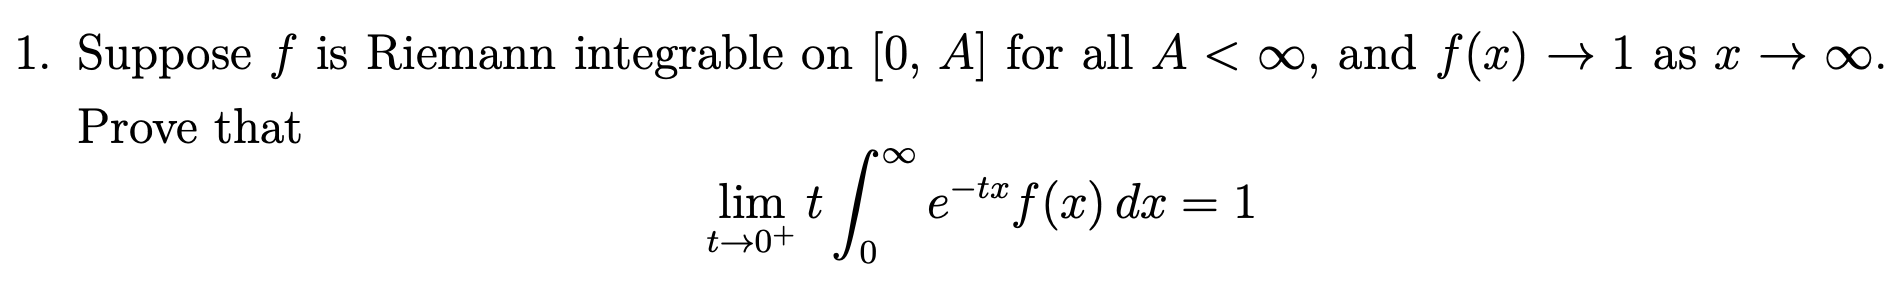
\includegraphics[height=3cm,width=18cm]{ahw23}
\end{question}
\begin{proof}
We can reduce the problem into proving 
\begin{align*}
\vi{\lim_{t\to 0^+}\int_0^\infty te^{-tx}f(x)dx-1=0}
\end{align*}
Notice that for each $t>0$, we have 
 \begin{align*}
1=\int_0^\infty te^{-tx}dx
\end{align*}
This then give us 
\begin{align*}
\int_0^\infty e^{-tx}f(x)dx-1&=\int_0^\infty te^{-tx}f(x)dx-\int_0^\infty te^{-tx}dx\\
&=\int_0^\infty te^{-tx}\big[f(x)-1 \big]dx
\end{align*}
Define $g(x)\triangleq f(x)-1$. Because $f\to 1$ at $\infty$, we know $g \to 0$ at infinity. We now reduce the problem into proving 
\begin{align*}
\vi{\lim_{t\to 0^+}\int_0^\infty te^{-tx}g(x)dx=0}
\end{align*}
Note that with simple computation 
\begin{align*}
\int_0^\infty te^{-tx}dx\text{ exists for all $t\inr^+$ }
\end{align*}
Then because we have $te^{-tx}\sim te^{-tx}f(x)$ as $x \to \infty$, we see 
\begin{align*}
\int_0^\infty te^{-tx}g(x)dx\text{ exists for all $t\inr^+$ by Integral Test and Limit Comparison Test
}
\end{align*}
Fix $\epsilon $. We now reduce the problem into proving 
\begin{align*}
\vi{\text{ finding $\delta$ such that }\abso{\int_0^\infty te^{-tx}g(x)dx}\leq \epsilon \text{ for all $t\in (0,\delta)$ }}
\end{align*}
Let $A$ be large enough such that $g(x)$ is  $\frac{\epsilon}{2}$-close to $0$ whenever $x\geq A$. Note that $g$ is bounded on $[A,\infty)$ and bounded on $[0,A]$ because $g$ is integrable on $[0,A]$. Now, let $M>\sup_{\R^+}\abso{g}$. We claim
 \begin{align*}
   \vi{\delta= \frac{-\ln (1-\frac{\epsilon}{2M})}{A}\text{ works }}
\end{align*}
Observe 
\begin{align*}
  \abso{\int_0^\infty te^{-tx}g(x)dx}&\leq \abso{\int_0^A te^{-tx}g(x)dx}+\abso{\int_A^\infty te^{-tx}g(x)dx}\\
  &\leq \int_0^A te^{-tx}\abso{g(x)}dx+ \int_A^\infty te^{-tx}\abso{g(x)}dx\\
  &\leq M\int_0^A te^{-tx}dx + \frac{\epsilon}{2}\int_A^\infty te^{-tx}dx\\
  &\leq  -Me^{-tx}\Big|_{x=0}^A +\frac{\epsilon}{2}\int_0^\infty te^{-tx}dx\\
  &\leq M(1-e^{-tA})+\frac{\epsilon}{2}\\
  &\leq M(1-e^{-\delta A})+\frac{\epsilon}{2}\\
  &=M(1-e^{\ln (1-\frac{\epsilon}{2M})})+\frac{\epsilon}{2}=\epsilon \vdone
\end{align*}

\end{proof}
\begin{question}{}{}
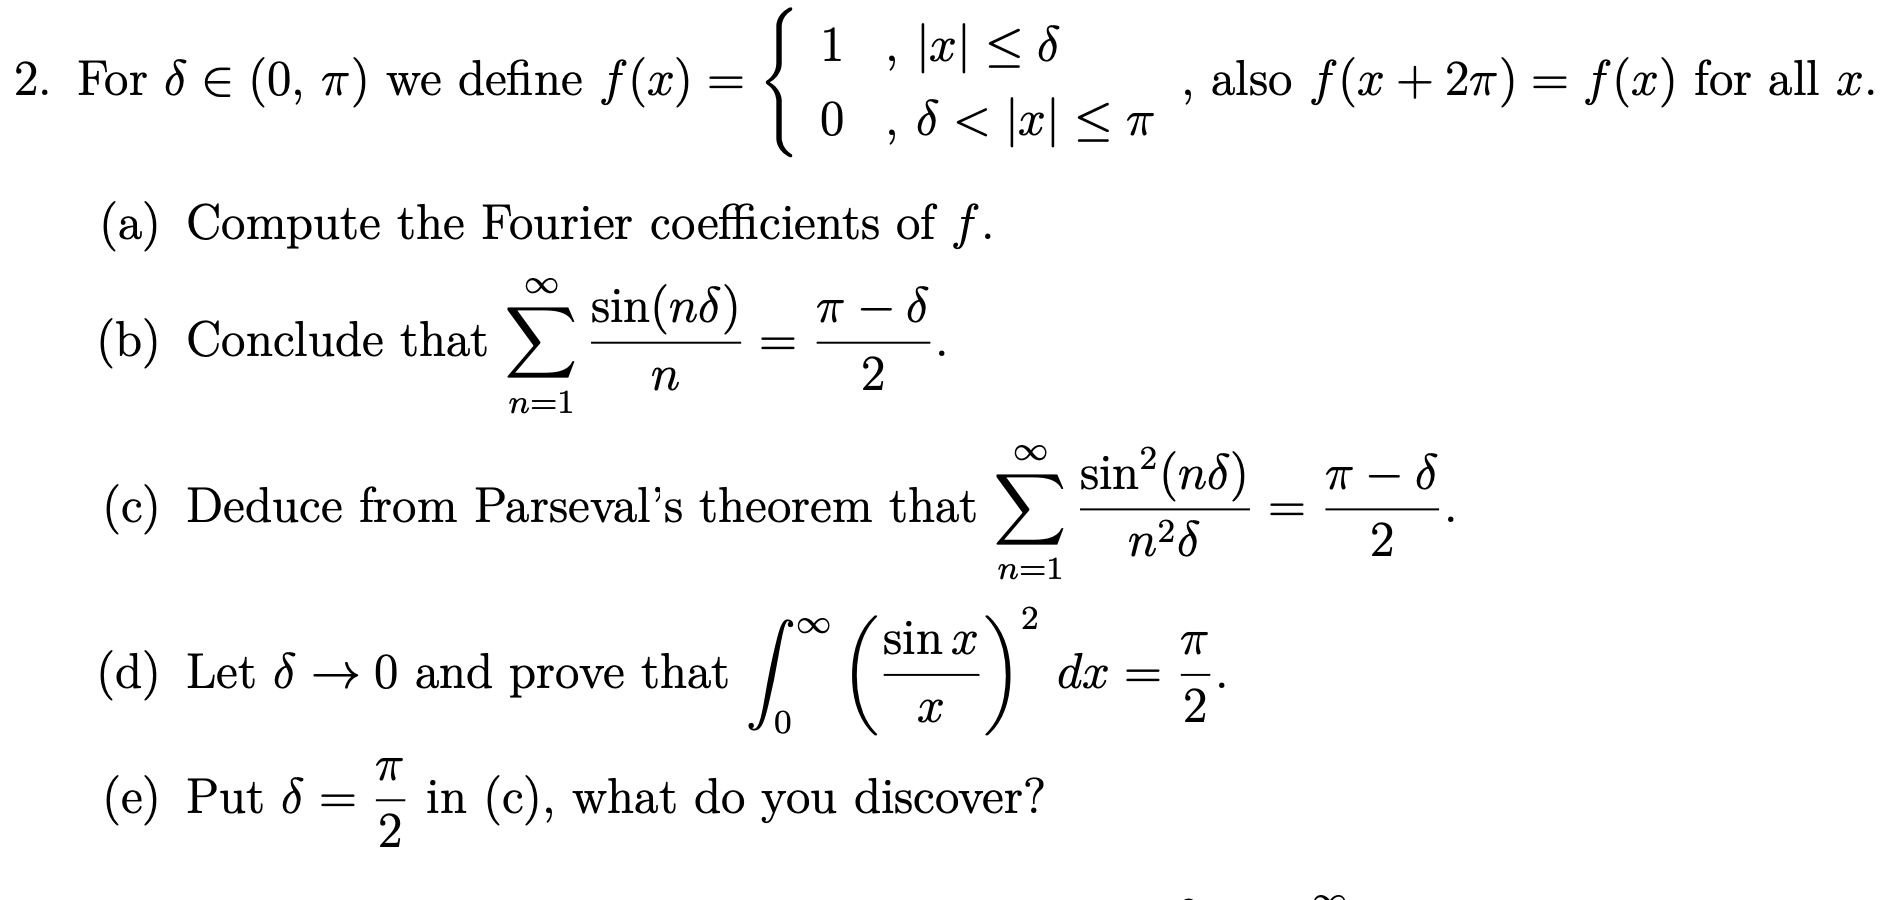
\includegraphics[height=9cm,width=18cm]{ahw22}
\end{question}
\begin{proof}
\textbf{(a)}\\

For $n\neq 0$, compute 
\begin{align*}
c_n &= \frac{1}{2\pi}\int_{-\pi}^{\pi}f(x)e^{-i nx}dx\\
&=\frac{1}{2\pi}\int_{-\delta}^\delta \cos (-nx)+ i \sin (nx)dx\\
&=\frac{1}{2\pi}\int_{-\delta}^\delta \cos (-nx)dx \hspace{0.5cm}(\because \text{ $\sin$ is odd function })\\
&=\frac{1}{2\pi} \cdot \frac{\sin (-nx)}{-n}\Big |_{x=-\delta}^{\delta}= \frac{ \sin (n\delta)}{n \pi }
\end{align*}
Compute 
\begin{align*}
c_0=\frac{1}{2\pi}\int^{\pi}_{-\pi}f(x)dx=\frac{\delta}{\pi}
\end{align*}
\textbf{(b)}\\

Note that $c_{-n}=c_n$. We then deduce that the Fourier Series of $f$ is 
\begin{align*}
\frac{\delta}{\pi}+\sum_{n=1}^\infty \frac{2\sin (n\delta)}{n\pi} e^{-i nx}
\end{align*}
Because $f$ is constant around $0$, it is clearly Lipschitz at $0$. We now deduce
 \begin{align*}
1=f(0)=\frac{\delta}{\pi} + \sum_{n=1}^\infty \frac{2 \sin (n\delta)}{n \pi }
\end{align*}
This implies 
\begin{align*}
\sum_{n=1}^\infty \frac{2\sin (n \delta)}{n\pi}=1-\frac{\delta}{\pi}
\end{align*}
which implies 
\begin{align*}
\sum_{n=1}^\infty \frac{\sin (n\delta)}{n}=(1-\frac{\delta}{\pi})\cdot \frac{\pi}{2}=\frac{\pi - \delta}{\pi}\cdot \frac{\pi}{2}=\frac{\pi -\delta}{2}
\end{align*}
\textbf{(c)} \\

Parseval's Theorem says 
\begin{align*}
\frac{1}{2\pi}\int_{-\pi}^{\pi}\abso{f(x)}^2dx=\sum_{-\infty}^\infty \abso{c_n}^2
\end{align*}
Clearly $f$ is Riemann-Integrable. Plugin our setting, we see 
\begin{align*}
\frac{1}{2\pi}\int_{-\pi}^\pi\abso{f}^2dx= \frac{\delta}{\pi}
\end{align*}
and
\begin{align*}
\sum_{-\infty}^\infty \abso{c_n}^2&=(\frac{\delta}{\pi})^2+ \sum_{n=1}^\infty 2\Big( \frac{\sin (n\delta)}{n \pi }\Big)^2\\
&=(\frac{\delta}{\pi})^2 + \frac{2}{\pi^2}\sum_{n=1}^\infty \frac{\sin^2 (n\delta)}{n^2} 
\end{align*}
This let us deduce 
\begin{align*}
\sum_{n=1}^\infty \frac{\sin ^2 (n\delta)}{n^2}=\frac{\pi^2}{2}\cdot \big(\frac{\delta}{\pi}-\frac{\delta^2}{\pi^2} \big)=\frac{\pi \delta -\delta^2}{2}
\end{align*}
So 
\begin{align*}
\sum_{n=1}^\infty \frac{\sin^2(n\delta)}{n^2 \delta}=\frac{\pi -\delta}{2}
\end{align*}
\textbf{(d)}\\

Fix $\epsilon $. Because $\int_0^\infty \frac{\sin^2}{x^2}dx$ absolutely converge, we can find $R$ satisfying
\begin{align*}
\abso{\int_R^\infty \frac{\sin^2 x}{x^2}dx}<\frac{\epsilon}{3}\text{ and }R>\frac{3}{\epsilon }
\end{align*}
Define $\delta_N \triangleq \frac{R}{N}$. Partition $[0,R]$ by $\set{0,R(\frac{1}{N}),R(\frac{2}{N}),\dots ,R }$. We see 
\begin{align*}
\sum_{n=1}^N \frac{\sin^2 (n\delta_N)}{(n\delta_N)^2}\delta_N\text{ is a Riemann Sum of Norm $\abso{\delta_N}$ }
\end{align*}
This implies that there exists $N_0$ such that 
\begin{align*}
\forall N>N_0, \abso{\sum_{n=1}^N \frac{\sin^2 (n\delta_N)}{(n\delta_N)^2}\delta_N- \int_0^R \frac{\sin^2 x}{x^2}dx}<\frac{\epsilon}{3}
\end{align*}
Fix $N>N_0$. Observe that 
 \begin{align*}
   \abso{\sum_{n=N+1}^\infty \frac{\sin^2 (n\delta_N)}{(n\delta_N)^2}\delta_N}&\leq \sum_{n=N+1}^\infty \frac{\sin^2 (n\delta_N)}{n^2 \delta_N}\\
&\leq \sum_{n=N+1}^\infty \frac{1}{n^2 \delta_N}\\
&=\frac{1}{\delta_N}\sum_{n=N+1}^\infty \frac{1}{n^2}\\
&\leq \frac{1}{\delta_N}\int_N^\infty \frac{1}{x^2}dx\hspace{0.5cm}(\because \frac{1}{x^2}\searrow )\\
&=\frac{1}{N\delta_N}=\frac{1}{R}<\frac{\epsilon}{3}
\end{align*}
We now see 
\begin{align*}
  &\abso{\sum_{n=1}^\infty \frac{\sin^2 (n\delta_N)}{(n\delta_N)^2}\delta_N- \int_0^\infty \frac{\sin^2 x}{x^2}dx}\\
  \leq &\abso{\sum_{n=1}^N \frac{\sin^2 (n\delta_N)}{(n\delta_N)^2}\delta_N - \int_0^R \frac{\sin^2 x}{x^2}dx}+\abso{\sum_{n=N+1}^\infty \frac{\sin^2  (n\delta_N)}{(n\delta_N)^2}\delta_N}+\abso{\int_R^{\infty}\frac{\sin^2 x}{x^2}dx}\\
  \leq & \frac{\epsilon }{3}+\frac{\epsilon}{3}+\frac{\epsilon}{3}=\epsilon 
\end{align*}
This now implies, for all $\epsilon $, we can find $R$ and a threshold $N_0$ corresponding to $R$ such that 
\begin{align*}
\forall N>N_0, \abso{\sum_{n=1}^\infty \frac{\sin^2 (n\delta_N)}{(n\delta_N)^2}\delta_N - \int_0^\infty \frac{\sin^2 x}{x^2}dx}\leq \epsilon 
\end{align*}
Then for $\epsilon_k=\frac{1}{k}$, we can find a sequence of real number $\delta_k\triangleq \frac{R_k}{N_k}\to 0$ such that 
\begin{align*}
\abso{\sum_{n=1}^\infty \frac{\sin^2 (n\delta_k)}{(n\delta_k)^2}\delta_k -\int_0^\infty \frac{\sin^2 x}{x^2}dx}\leq \frac{1}{k}
\end{align*}
Because we know 
 \begin{align*}
\sum_{n=1}^\infty \frac{\sin^2 (n\delta_k)}{(n\delta_k)^2}\delta_k =\frac{\pi -\delta_k}{2}
\end{align*}
We now see for each $\epsilon '$, because $\delta_k \to 0$, we can find $k$ large enough such that  
\begin{align*}
  \abso{\int_0^\infty \frac{\sin^2 x}{x^2}dx-\frac{\pi}{2}}&=\abso{{\int_0^\infty \frac{\sin^2 x}{x^2}dx- \frac{\pi-\delta_k}{2}- \frac{\delta_k}{2}}}\\
  &\leq \abso{\int_0^\infty \frac{\sin^2 x}{x^2}dx- \sum_{n=1}^{\infty} \frac{\sin^2 (n\delta_k)}{(n\delta_k)^2}\delta_k}+ \frac{\delta_k}{2}\\
  &\leq \frac{1}{k}+\frac{\delta_k}{2}<\epsilon ' 
\end{align*}
\textbf{(e)}\\

Put $\delta=\frac{\pi}{2}$. We have
\begin{align*}
\frac{\pi}{4}&=\frac{\pi-\delta}{2}\\
&=\frac{2}{\pi}\cdot\sum_{n=1}^\infty \frac{\sin^2 \frac{\pi}{2}n}{n^2}
\end{align*}
This then implies 
\begin{align*}
\sum_{n=1}^\infty \frac{1}{(2n-1)^2}=\frac{\pi^2}{8}
\end{align*}

\end{proof}
\begin{question}{}{}
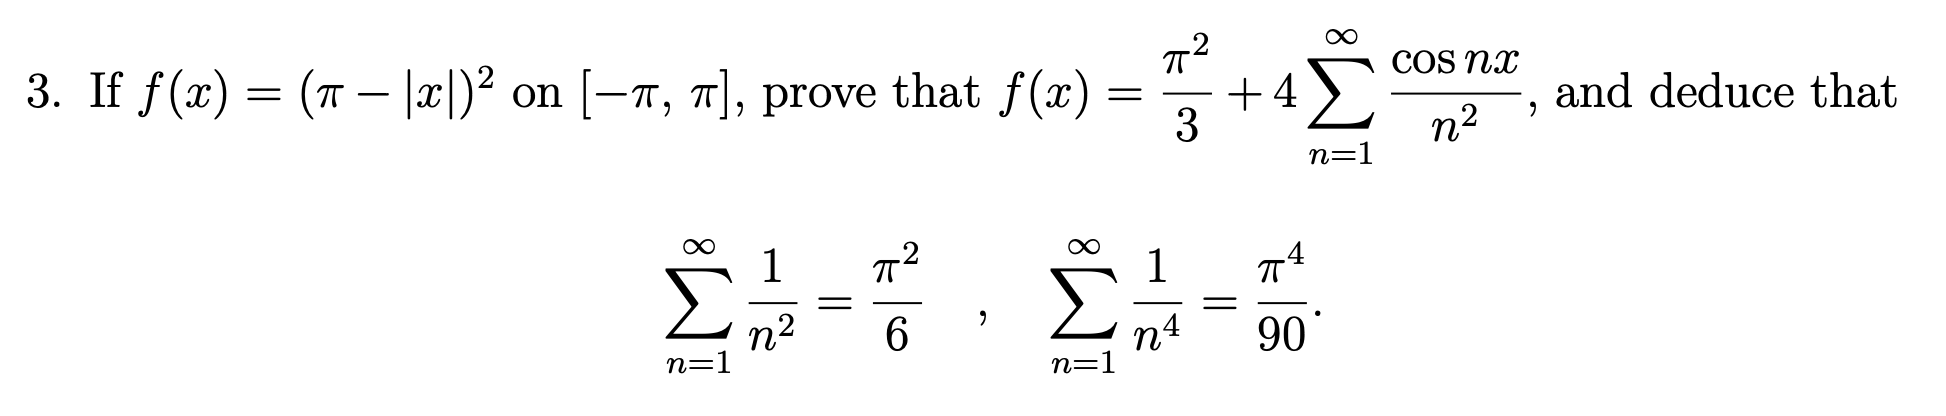
\includegraphics[height=4cm,width=18cm]{ahw29}
\end{question}
\begin{proof}
Compute Fourier coefficient 
\begin{align*}
c_0&=\frac{1}{2\pi}\int_{-\pi}^\pi (\pi - \abso{x})^2dx=\frac{\pi^2}{3}
\end{align*}
and 
\begin{align*}
c_n&=\frac{1}{2\pi}\int_{-\pi}^\pi (\pi -\abso{x})^2 e^{-inx}dx\\
&=\frac{2}{n^2}
\end{align*}
Note that $f$ is an even function, that  $f'(x)=2(x-\pi)$ on $(0,\pi ]$ and that 
\begin{align*}
f'(0)=\lim_{x\to 0^+} \frac{(\pi - \abso{x})^2 - \pi^2}{x}=\lim_{x\to 0^+} \frac{-2\pi x +x^2}{x}=-2\pi 
\end{align*}
This now let us deduce 
\begin{align*}
\abso{f'}\leq  2\pi \text{ on $[-\pi , \pi]$ }
\end{align*}
Which implies $f$ is  $2\pi$-Lipschitz on $[-\pi , \pi ]$. This tell us that the Fourier Series $s_N(f;x)$ converge to $f$, meaning 
\begin{align*}
f(x)=\sum_{-\infty}^\infty c_ne^{-i nx}&=\frac{\pi^2}{3}+\sum_{-\infty, n\neq 0}^\infty \frac{2}{n^2}\cdot \big(\cos (-nx)+ i \sin (-nx) \big)\\
&=\frac{\pi^2}{3}+\sum_{n=1}^\infty \frac{4 \cos nx}{n^2}=\frac{\pi^2}{3}+4\sum_{n=1}^\infty \frac{\cos nx}{n^2}
\end{align*}
We now can deduce
\begin{align*}
f(0)&=\pi^2\\
&=\frac{\pi^2}{3}+4 \sum_{n=1}^\infty \frac{1}{n^2}
\end{align*}
This then implies  
\begin{align*}
\sum_{n=1}^\infty \frac{1}{n^2}=\frac{\pi^2}{6}
\end{align*}
Because $f$ is continuous on $[-\pi , \pi]$, we know $f$ is Riemann-Integrable. Then Parseval's Theorem assert 
\begin{align*}
\frac{1}{2\pi} \int_{-\pi}^{\pi} \abso{f}^2 dx= \sum_{-\infty}^\infty \abso{c_n}^2
\end{align*}
Now compute 
\begin{align*}
\frac{1}{2\pi} \int_{-\pi }^\pi \abso{f}^2dx&=\frac{1}{2\pi}\int_{-\pi}^{\pi} (\pi - \abso{x})^4dx\\
&=\frac{1}{\pi}\int_0^\pi (\pi -x)^4 dx\hspace{0.5cm}(\because (\pi -\abso{x})^4 \text{ is even })\\
&=\frac{1}{\pi} \cdot \frac{(\pi -x )^5}{-5}\Big|_{x=0}^\pi= \frac{\pi^4}{5}
\end{align*}
and 
\begin{align*}
\sum_{-\infty}^\infty \abso{c_n}^2= \frac{\pi^4}{9}+ 2\sum_{n=1}^\infty \frac{4}{n^4}
\end{align*}
This now implies 
\begin{align*}
\sum_{n=1}^\infty \frac{1}{n^4}= \frac{1}{8}\cdot (\frac{\pi^4}{5}-\frac{\pi^4}{9})=\frac{\pi^4}{90}
\end{align*}
\end{proof}
\begin{question}{}{}
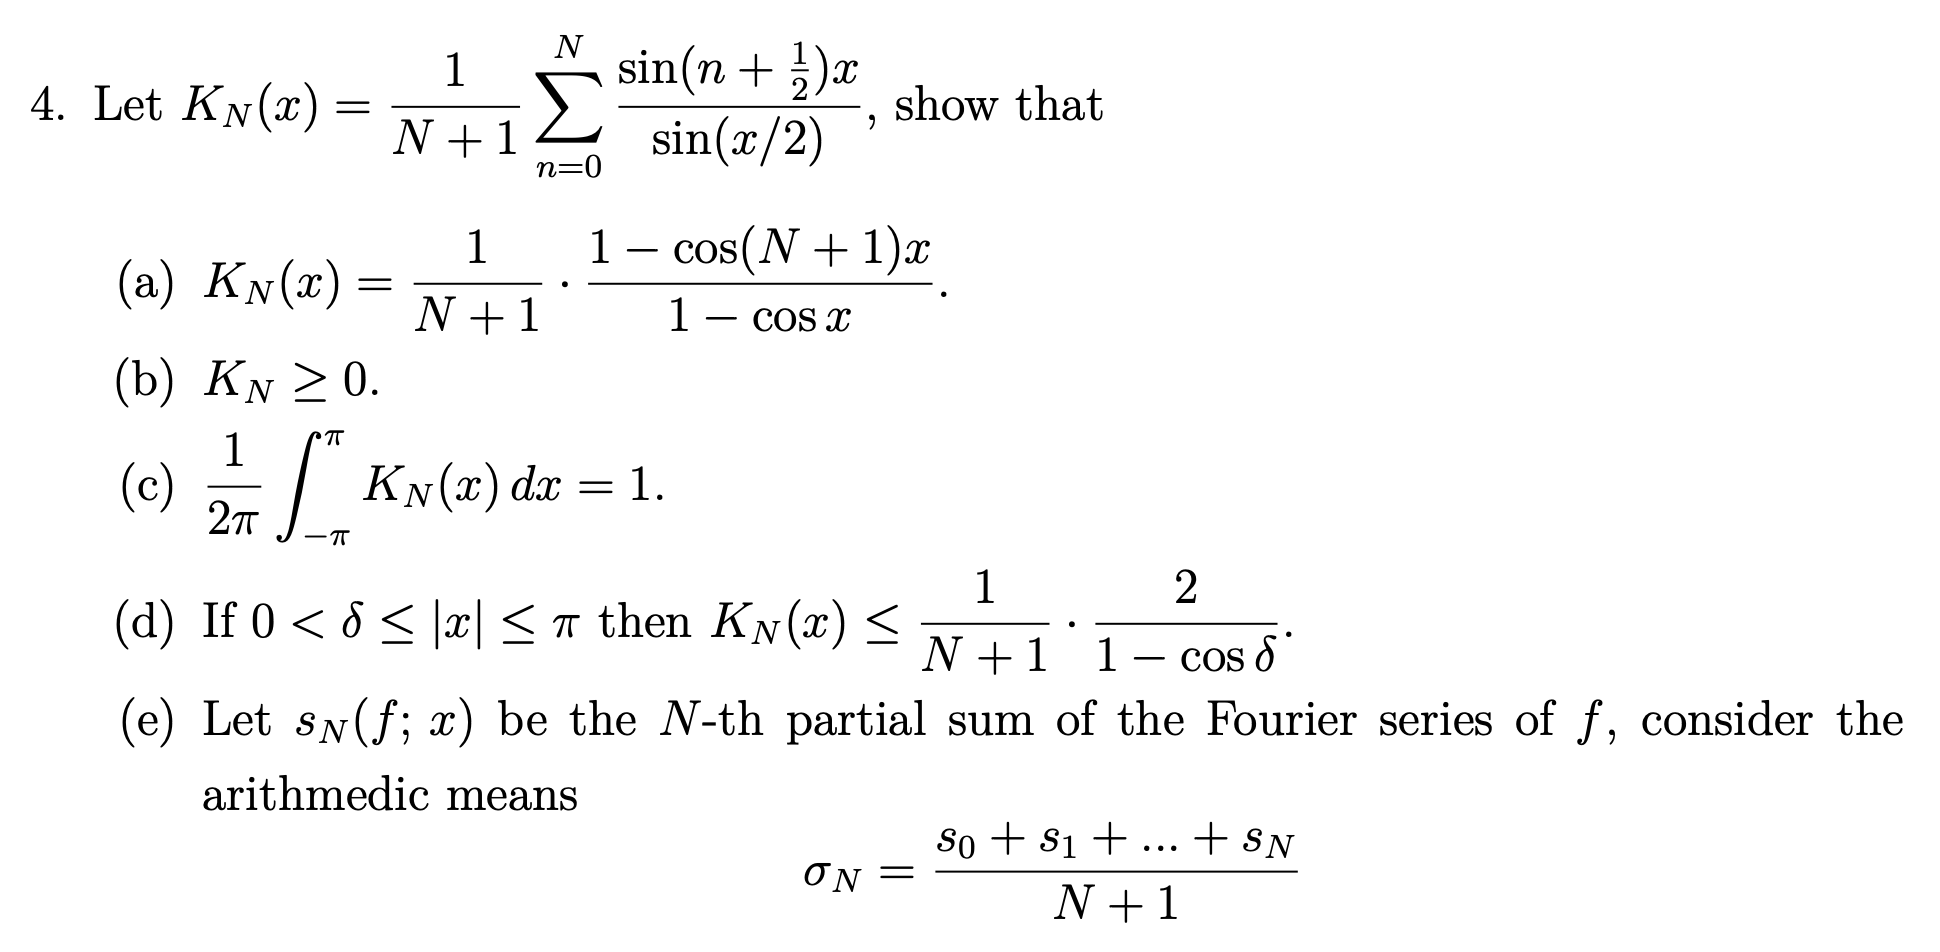
\includegraphics[height=10cm,width=18cm]{ahw28}
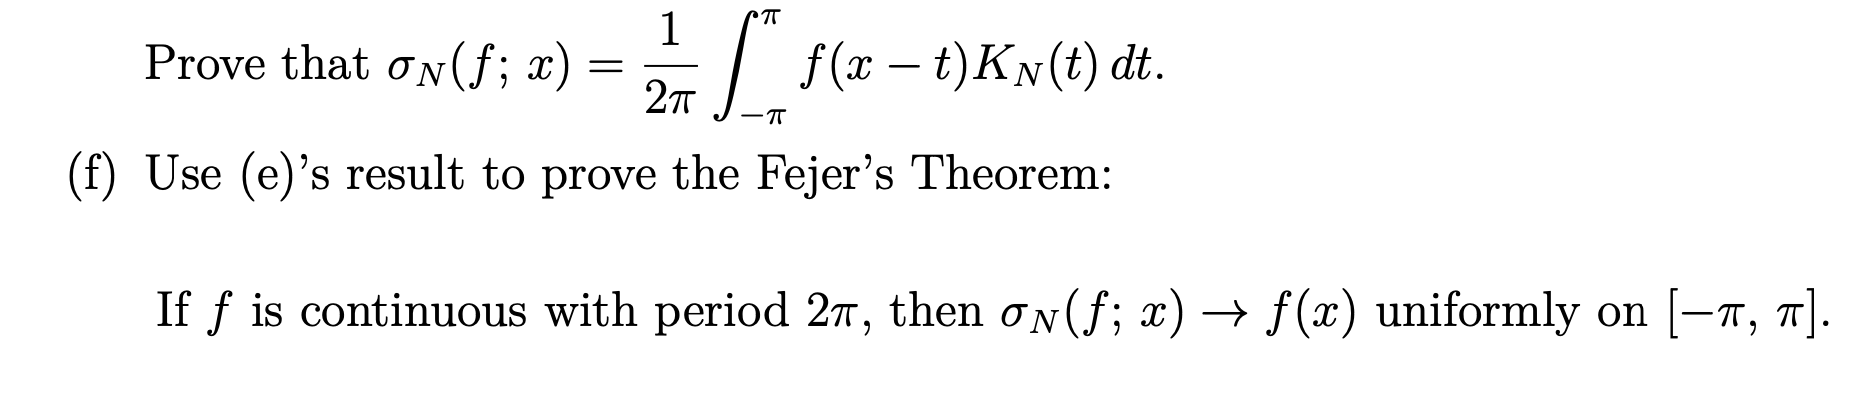
\includegraphics[height=4cm,width=18cm]{ahw27}
\end{question}
\begin{proof}
Proving $(a)$ can be reduced to proving 
\begin{align*}
\vi{\sum_{n=0}^N \frac{\sin (n+\frac{1}{2})x}{\sin (\frac{x}{2})}=\frac{1- \cos (N+1)x}{1-\cos x}}
\end{align*}
Using $\sin \alpha \sin \beta = \frac{1}{2}\Big(\cos (\alpha -\beta )-\cos (\alpha +\beta ) \Big)$ to compute 
\begin{align*}
\sum_{n=0}^N \frac{\sin (n+\frac{1}{2})x}{\sin (\frac{x}{2})}&= \frac{1-\cos x}{1- \cos x} \sum_{n=0}^N \frac{\sin (n+\frac{1}{2})x}{\sin (\frac{x}{2})}\\
&=\frac{2 \sin^2 (\frac{x}{2})}{1- \cos x} \sum_{n=0}^N \frac{\sin (n+\frac{1}{2})x}{\sin (\frac{x}{2})}\\
&=\frac{1}{1-\cos x}\sum_{n=0}^N 2\sin(\frac{x}{2})\sin (n+\frac{1}{2})x\\
&=\frac{1}{1- \cos x}\sum_{n=0}^N \cos (-nx)- \cos (n+1)x\\
&=\frac{1}{1- \cos x}\sum_{n=0}^N \cos (nx)- \cos (n+1)x=\frac{1- \cos (N+1)x}{1- \cos x}\vdone
\end{align*}
\textbf{(b)}\\

Notice that $\cos x < 1$ and $\cos (N+1)x\leq 1\hspace{0.5cm}(\because K_N\text{ is only well defined on $(0, 2\pi)$ })$. This then implies 
\begin{align*}
1-\cos x>0\text{ and }1-\cos (N+1)x\geq 0
\end{align*}
Then we can deduce 
\begin{align*}
K_N(x)=\frac{1}{N+1}\cdot \frac{1- \cos (N+1)x}{1-\cos x}\geq 0
\end{align*}
\textbf{(c)}\\

We first compute the Dirchlet Kernel $D_N$
\begin{align*}
D_N(x)&=\sum_{-N}^N e^{-i nx}\\
&=\frac{e^{i(-N)x}-e^{i(N+1)x}}{1-e^{ix}}\\
&=\frac{e^{i(-N-\frac{1}{2})x}-e^{i(N+\frac{1}{2})x}}{e^{i\frac{-1}{2}x}-e^{i\frac{1}{2}x}}\\
&=\frac{2i\sin((-N-\frac{1}{2})x)}{2i \sin (\frac{-1}{2}x)}= \frac{\sin (N+\frac{1}{2})x}{\sin (\frac{x}{2})}
\end{align*}
and 
\begin{align*}
D_N(x)=\sum_{-N}^N e^{-i nx}=1+2\sum_{n=1}^N \cos nx 
\end{align*}
Now we can compute 
\begin{align*}
\frac{1}{2\pi}\int_{-\pi}^\pi K_N(x)dx&=\frac{1}{2\pi}\int_{-\pi}^{\pi} \frac{1}{N+1}\sum_{n=0}^N \frac{\sin (n+\frac{1}{2})x}{\sin \frac{x}{2}}dx\\
&=\frac{1}{2\pi (N+1)}\sum_{n=0}^N \int_{-\pi}^{\pi} D_n(x)dx\\
&=\frac{1}{2\pi (N+1)}\sum_{n=0}^N \int_{-\pi}^{\pi} (1+2 \sum_{k=1}^n \cos kx)dx\\
&=\frac{1}{2\pi(N+1)}\sum_{n=0}^N 2\pi=1\hspace{0.5cm}(\because \int_{-\pi}^{\pi}\cos kx=0)
\end{align*}
\textbf{(d)}\\

Suppose $0<\delta\leq \abso{x}\leq \pi$. Observe
\begin{align*}
K_N(x)&=\frac{1}{N+1}\cdot \frac{1- \cos (N+1)x}{1-\cos x}\\
&\leq  \frac{1}{N+1}\cdot \frac{2}{1 - \cos x}\hspace{0.5cm}(\because \cos x <1)\\
&\leq \frac{1}{N+1}\cdot \frac{2}{1- \cos \delta}\hspace{0.5cm}(\because 0<\delta \leq \abso{x}\leq \pi \implies \cos x\leq \cos \delta <1 )
\end{align*}
\textbf{(e)}\\

Compute 
\begin{align*}
\sigma_N(f;x)&=\frac{(s_0+ \cdots +s_N)}{N+1}(f;x)\\
&=\frac{1}{N+1}\sum_{k=0}^N s_k(f;x)\\
&=\frac{1}{N+1}\sum_{k=0}^N \sum_{n=-k}^k c_ne^{i nx}\\
&=\frac{1}{N+1}\sum_{k=0}^N \sum_{n=-k}^k \frac{1}{2\pi}\int_{-\pi}^\pi f(t)e^{-i nt}dte^{inx}\\
&=\frac{1}{N+1}\sum_{k=0}^N \frac{1}{2\pi}\sum_{n=-k}^{k}\int_{-\pi}^{\pi}f(t)e^{in(x-t)}dt\\
&=\frac{1}{N+1}\sum_{k=0}^N \frac{1}{2\pi}\int_{-\pi}^{\pi}f(t)\sum_{n=-k}^{k}e^{in(x-t)}dt\\
&=\frac{1}{N+1}\sum_{k=0}^N \frac{1}{2\pi} \int_{-\pi}^{\pi}f(t)D_k(x-t)dt\\
&=\frac{1}{(N+1)2\pi}\sum_{k=0}^N \int^{x-\pi}_{x+\pi} -f(x-u)D_k(u)du\hspace{0.5cm}(\because u=x-t)\\
&=\frac{1}{(N+1)2\pi}\sum_{k=0}^N \int_{x-\pi}^{x+\pi}f(x-u)D_k(u)du\\
&=\frac{1}{(N+1)2\pi}\sum _{k=0}^{N}\int_{-\pi}^{\pi}f(x-u)D_k(u)du\hspace{0.5cm}(\because \text{ periodicity of $D_k$ and $f$ })\\
&=\frac{1}{2\pi}\int_{-\pi}^{\pi}f(x-u)\cdot\Big( \frac{1}{N+1}\sum_{k=0}^N D_k(u)\Big)du\\
&=\frac{1}{2\pi}\int_{-\pi}^{\pi} f(x-u)K_N(u)du
\end{align*}
\textbf{(e)}\\

Fix $\epsilon $. We wish 
\begin{align*}
\vi{\text{ to find $N'$ such that for all $N>N'$ and  $x \inr$ we have }\abso{\sigma_N(f;x)-f(x)}\leq \epsilon }
\end{align*}
Because $f$ is continuous with period $2\pi$, we know $f$ is uniformly continuous on $\R$. We then can fix $\delta$ small enough such that 
\begin{align*}
\sup_{\abso{t}\leq \delta} \abso{f(x-t)-f(x)}<\frac{\epsilon}{2}
\end{align*}
Also, we can fix $M>\sup_{[-\pi,\pi]}\abso{f}$. Define $Q_\delta=\frac{4M(\pi-\delta)}{\pi (1-\cos \delta)}$. We claim 
\begin{align*}
\vi{\text{ $N'>\frac{2Q_\delta}{\epsilon }$ works }}
\end{align*}
Fix $N>N'$ and  $x \inr$. Using $\frac{1}{2\pi}\int_{-\pi}^{\pi}K_N(t)dt=1$ and $K_N\geq 0$, see 
\begin{enumerate}[label=(\alph*)]
  \item $\frac{1}{2\pi}\int_{-\pi}^{\pi}K_N(t)dt=1$ 
  \item $K_N\geq 0$
  \item $\pi \geq \abso{x}\geq \delta \implies K_N(x)\leq \frac{1}{N+1}\cdot \frac{2}{1-\cos \delta}$
\end{enumerate}
\begin{align*}
\abso{\sigma_N(f;x)-f(x)}&=\abso{\frac{1}{2\pi}\int_{-\pi}^{\pi}f(x-t)K_N(t)dt-f(x)\frac{1}{2\pi}\int_{-\pi}^{\pi}K_N(t)dt}\\
&=\frac{1}{2\pi}\int_{-\pi}^{\pi}\abso{f(x-t)-f(x)}K_N(t)dt\\
&=\frac{1}{2\pi}\int_{-\delta}^{\delta} \abso{f(x-t)-f(x)}K_N(t)dt+\frac{2(\pi -\delta)2M}{2\pi}\cdot \frac{1}{N+1}\cdot \frac{2}{1-\cos \delta}\\
&\leq \frac{1}{2\pi}\int_{-\pi}^{\pi}\frac{\epsilon }{2}K_N(t)dt+\frac{4M(\pi -\delta)}{(N+1)\pi(1-\cos \delta)}\\
&=\frac{\epsilon}{2}+\frac{4M(\pi-\delta)}{\frac{2Q_\delta}{\epsilon }\pi(1-\cos \delta)}=\frac{\epsilon}{2}+\frac{\epsilon}{2}=\epsilon\vdone
\end{align*}
\end{proof}
\begin{question}{}{}
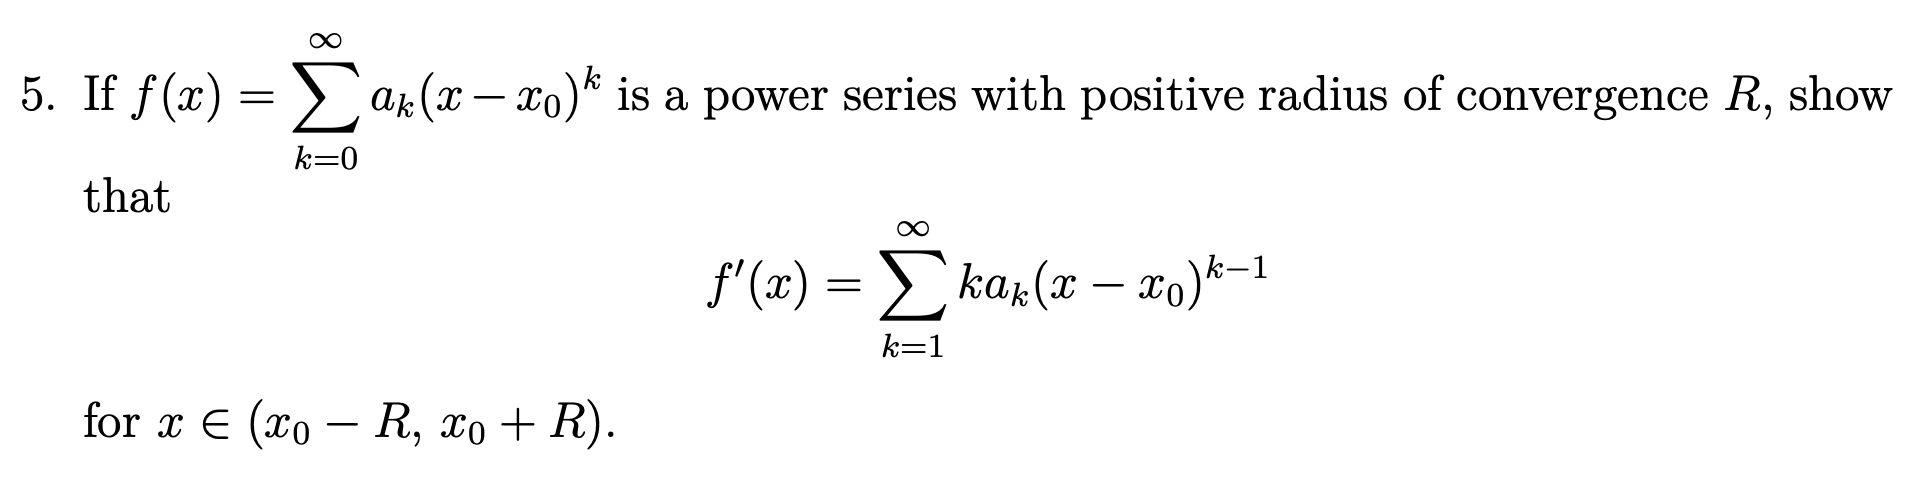
\includegraphics[height=5cm,width=18cm]{ahw26}
\end{question}
\begin{theorem}
\textbf{(Power Series are Smooth)} Given a power series $(a,c_n)$ of convergence radius $R$, if we define $f:D_R(a)\rightarrow \C$ by 
\begin{align*}
f(z)=\sum_{n=0}^\infty c_n (z-a)^n 
\end{align*}
Then 
\begin{align*}
f\text{ is of class }C^\infty\text{ on $D_{R}(a)$ and $f^{(k)}(z)=\sum_{n=k}^\infty \frac{n!}{(n-k)!}c_n(z-a)^{n-k}$  on $D_R(a)$}
\end{align*}
\end{theorem}
\begin{proof}
We prove by induction. Base case $k=0$ is trivial. Fix $k\geq 0$. Suppose we have 
\begin{align*}
f^{(k)}(z)=\sum_{n=k}^{\infty} \frac{n!}{(n-k)!}c_n(z-a)^{n-k}\text{ on $D_R(a)$ }
\end{align*}
We are required to prove 
\begin{align*}
\vi{f^{(k+1)}(z)=\sum_{n=k+1}^\infty \frac{n!}{(n-k-1)!}c_n(z-a)^{n-k-1}\text{ on }D_R(a)}
\end{align*} 
Set $f_m$ 
 \begin{align*}
f_m(z)\triangleq \sum_{n=k}^{k+m} \frac{n!}{(n-k)!}c_n(z-a)^{n-k}
\end{align*}
We have 
\begin{align}
\label{PS1}
f_m \to f^{(k)}\text{ pointwise on $D_R(a)$ and }f'_m (z)= \sum_{n=k+1}^{k+m}\frac{n!}{(n-k-1)!}c_n(z-a)^{n-k-1}
\end{align}
We abstract our problem into proving 
\begin{align*}
  \vi{f'_m \to f^{(k+1)}\text{ pointwise on $D_R(a)$ }}
\end{align*}
Fix $z_0 \in D_R(a)$. We only wish to prove 
\begin{align*}
\vi{(f^{(k)})'(z_0)=\lim_{m\to \infty}f'_m(z_0)}
\end{align*}
Fix $\epsilon $ such that $\abso{z_0-a}< R-\epsilon $. By \myref{Equation}{PS1}, using \myref{Theorem}{UCaD} (Uniform Convergence and Differentiaiton). We only have to prove 
\begin{align*}
  \vi{f'_m\text{ uniformly converge on $\overline{D}_{R-\epsilon }$ }}
\end{align*}
Note that 
\begin{align*}
f'_m(z)=\sum_{n=0}^{m-1} \frac{(n+k+1)!}{n!}c_{n+k+1}(z-a)^n
\end{align*}
so we can compute the radius of convergence for $f'_m$
\begin{align*}
\limsup_{n\to\infty} \sqrt[n]{\frac{(n+k+1)!}{n!}\abso{c_{n+k+1}}}&=\limsup_{n\to\infty} \sqrt[n]{\abso{c_{n+k+1}}} \\
&=\limsup_{n\to\infty} \sqrt[n]{\abso{c_n}}=R 
\end{align*}
Together by Cauchy-Hadamrd (absolute convergent on $a+R-\epsilon $) and M-test show that 
\begin{align*}
\sum_{n=0}^\infty \frac{(n+k+1)!}{n!}c_{n+k+1}(z-a)^n \text{ uniformly converge on $\overline{D}_{R-\epsilon }(a)$ }\vdone
\end{align*}
\end{proof}
\begin{question}{}{}
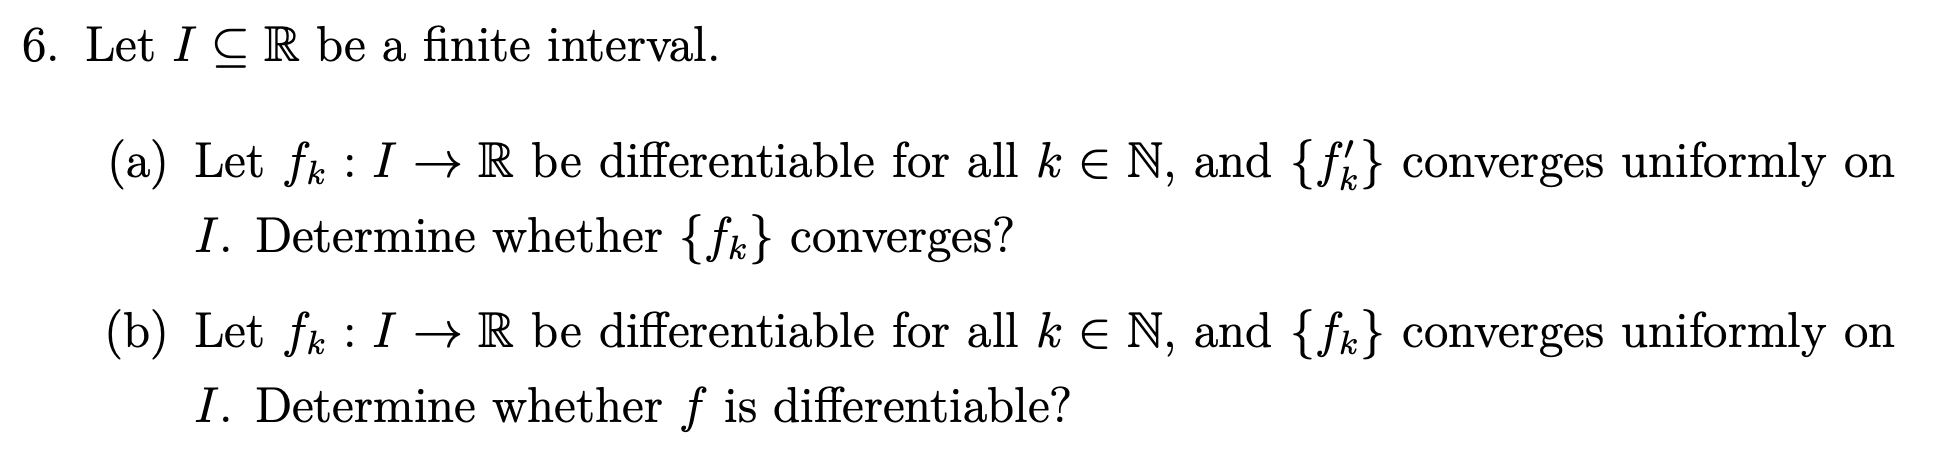
\includegraphics[height=8cm,width=18cm]{ahw25}
\end{question}
\begin{proof}
\textbf{(a)}
No. Let $f_k=k$. It is then a trivial counter example. \\

\textbf{(b)}
No. Consider $\abso{x}$. The function $\abso{x}$ is continuous on $[-1,1]$ but not differentiable on $x=0$. By Weierstrass approximation Theorem, we know there exists a sequence of polynomials on $[-1,1]$ uniformly converge to $\abso{x}$, and they clearly all are differentiable. 
\end{proof}
\begin{question}{}{}
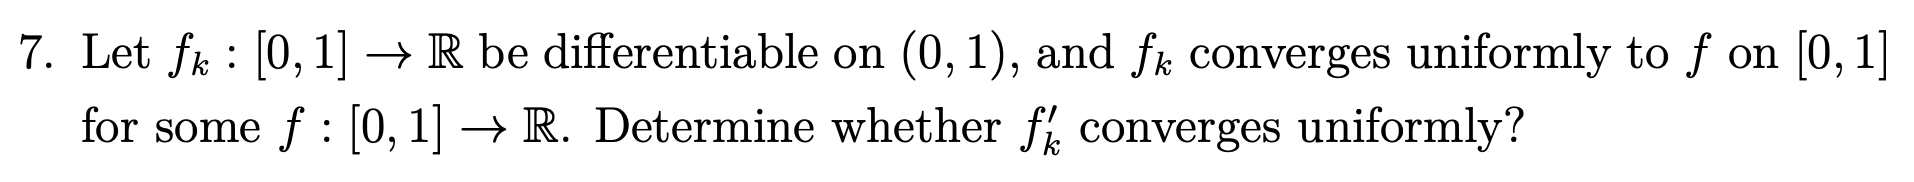
\includegraphics[height=3cm,width=18cm]{ahw24}
\end{question}
\begin{proof}
No. Consider 
\begin{Example}{\textbf{(Derivative won't necessarily converge to the right place)}}{}
\begin{align*}
X=\R \text{ and }f_n(x)=\frac{\sin nx}{\sqrt{n} }
\end{align*}
Compute 
\begin{align*}
f'(x)=0 \text{ and }f'_n(x)=\sqrt{n} \cos nx
\end{align*}
\end{Example}
$f'_n(0) \to \infty$ shows that $f'_n$ doesn't even have to be pointwise convergence. Note that the fact $f_k$ uniformly converge can be easily proved by choosing  $n>\frac{1}{\epsilon ^2}$  
\end{proof}
\begin{question}{}{}
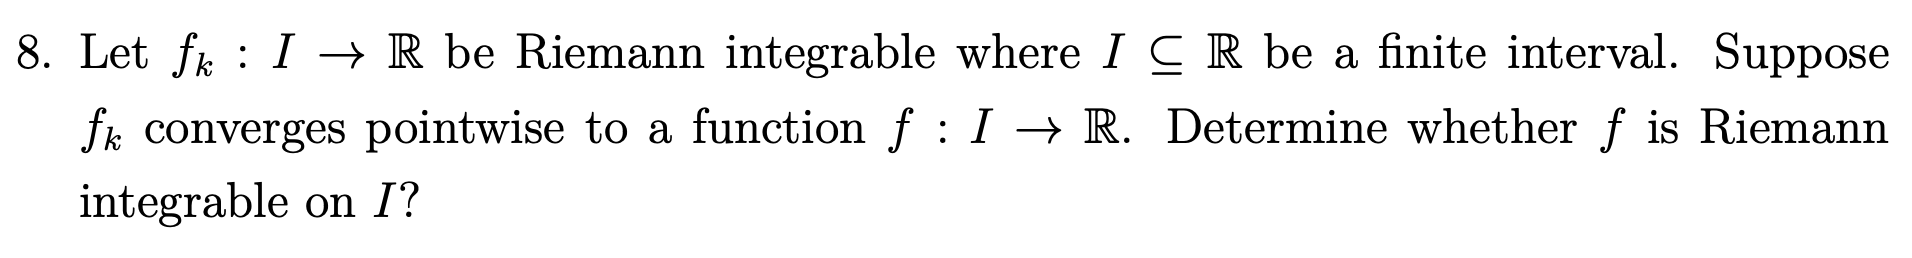
\includegraphics[height=3cm,width=18cm]{ahw21}
\end{question}
\begin{proof}
No. Consider 
\begin{Example}{\textbf{(Riemann-integrable functions Pointwise Converge to a Non-Riemann-integrable function)}}{}
\begin{align*}
X=[-1,1]\text{ and }f_m(x)=\lim_{n\to \infty} (\cos m! \pi x)^{2n}
\end{align*}
\end{Example}
Because $\cos$ has range $[-1,1]$, we know that 
\begin{align*}
m!x \inz \iff  f_m(x)\neq 0
\end{align*}
This tell us that for all $x\inr\setminus \Q$, $f_m(x)=0$, and that for all $x\inq$, we have $f_n(x)=1$ for large enough $n$, with some simple computation.\\

Then, we see that 
\begin{align*}
f_n \to \textbf{1}_\Q\text{ pointwise }
\end{align*}
Now, notice that for all fixed $m$, if  $m!x\inz$, we must have 
\begin{align*}
x=\frac{p}{m!}\text{ for some $p\inz$ }
\end{align*}
Such $x$ in bounded domain must then happen only finite amount of time. This show  $f_n$ are all continuous almost everywhere and thus integrable, while $\textbf{1}_\Q$, the function to which they converge, is not, as it is discontinuous almost everywhere.  
\end{proof}
\section{Uniform Convergence on Integration and Differentiation}
\begin{theorem}
\label{RIFac}
\textbf{(Riemann-Integration and Uniform Convergence)} Given a function $\alpha :[a,b]\rightarrow \R$ and a sequence of functions $f_n:[a,b]\rightarrow \R$ such that 
\begin{enumerate}[label=(\alph*)]
  \item $\alpha $ increase on $[a,b]$ 
  \item $\int_a^b f_nd\alpha $ exists for all $n\inn$ 
  \item $f_n \to f $ uniformly on $[a,b]$ 
\end{enumerate}
Then 
\begin{align*}
  \lim_{n\to \infty}\int_a^b f_n d\alpha \text{ exists and }\int_a^b fd\alpha =\lim_{n\to \infty}\int_a^b f_nd\alpha 
\end{align*}
\end{theorem}
\begin{proof}
We first prove 
\begin{align*}
\vi{\int_a^b fd\alpha \text{ exists }}
\end{align*}
Fix $\epsilon $. We wish to prove 
\begin{align*}
\vi{\overline{\int_a^b}fd\alpha - \underline{\int_a^b}fd\alpha < \epsilon }
\end{align*}
Let $\epsilon _n = \norm{f_n-f}_\infty$. Because $f_n \to f$ uniformly, we know 
\begin{align*}
\text{ there exists $n\inn$ such that $\epsilon _n=\norm{f_n-f}_\infty < \frac{\epsilon }{2\big[\alpha (b)-\alpha (a) \big]}$ }
\end{align*}
Because $\alpha $ increase, by definition of $\epsilon _n$, we see 
\begin{align*}
\int_a^b (f_n-\epsilon _n)d\alpha \leq \underline{\int_a^b}fd\alpha \leq \overline{\int_a^b}fd\alpha \leq \int_a^b (f_n+\epsilon_n) d\alpha  
\end{align*}
Because $\epsilon _n <\frac{\epsilon}{2\big[\alpha (b)-\alpha (a) \big]}$, we now see 
\begin{align*}
  \overline{\int_a^b}fd\alpha -\underline{\int_a^b}fd\alpha &\leq \int_a^b (f_n+\epsilon _n)d\alpha -\int_a^b (f_n-\epsilon _n)d\alpha \\
&=\int_a^b (2\epsilon _n)d\alpha<2 \epsilon_n \cdot \big[\alpha (b)-\alpha (a) \big] = \epsilon \vdone
\end{align*}
We now prove 
\begin{align*}
  \blue{\int_a^b f_n d\alpha \to \int_a^b fd\alpha \text{ as $n \to \infty $ }}
\end{align*}
Fix $\epsilon $. We wish 
\begin{align*}
\blue{\text{ to find $N$ such that }\forall n>N,\abso{\int_a^b f_nd\alpha-\int_a^b fd\alpha }<\epsilon  }
\end{align*}
Recall the definition $\epsilon_n= \norm{f_n-f}_\infty$. Because $\epsilon _n \to 0$, we know 
\begin{align}
\label{CuU1}
\text{ there exists $N$ such that }\forall n>N, \epsilon_n < \frac{\epsilon }{\alpha (b)-\alpha (a)}
\end{align}
We claim 
\begin{align*}
\blue{\text{ such $N$ works }}
\end{align*}
Fix $n>N$. From \myref{Equation}{CuU1}, we see
 \begin{align*}
  \abso{\int_a^b f_nd\alpha -\int_a^b fd\alpha }&=\abso{\int_a^b (f_n-f)d\alpha }\\
  &\leq \int_a^b \abso{f_n-f}d\alpha \\
  &\leq \int_a^b \epsilon_n d\alpha =\epsilon_n \big[\alpha (b)-\alpha (a) \big]<\epsilon \bdone
\end{align*}


\end{proof}
\begin{mdframed}
Before the next Theorem, let's see three examples why this time we don't (can't) use the hypothesis: $f_n \to f$ uniformly. 
\begin{Example}{\textbf{(Differentiable functions are NOT closed under uniform convergence)}}{}
\begin{align*}
X=[-1,1]\text{ and }f(x)=\abso{x}
\end{align*}
By Weierstrass approximation Theorem, there is a sequence of polynomials (differentiable) that uniformly converge to $f$, which is not differntiable at  $0$. 
\end{Example}
\begin{Example}{\textbf{(Derivative won't necessarily converge to the right place)}}{}
\begin{align*}
X=\R \text{ and }f_n(x)=\frac{\sin nx}{\sqrt{n} }
\end{align*}
Compute 
\begin{align*}
f'(x)=0 \text{ and }f'_n(x)=\sqrt{n} \cos nx
\end{align*}
\end{Example}
\begin{Example}{\textbf{(Derivative won't necessarily converge to the right place)}}{}
\begin{align*}
X=\R \text{ and }f_n(x)=\frac{x}{1+nx^2}
\end{align*}
Compute 
\begin{align*}
f=\tilde{0} \text{ and }f'_n(0)=1
\end{align*}
\end{Example}
Informally speaking, these examples together with the fact integral are closed under uniform convergence (\myref{Theorem}{RIFac}) should give you some ideas that differentiation and integration although are operations inverse to each other, are NOT symmetric. There is a certain hierarchy on continuous functions on a fixed compact interval. Thus, we have the next Theorem in its form. 
\end{mdframed}
\begin{theorem}
\label{UCaD}
\textbf{(Uniform Convergence and Differentiation)} Given a sequence of function $f_n:[a,b]\rightarrow \R$ such that 
\begin{enumerate}[label=(\alph*)]
  \item $f_n(x_0)\to L$ for some $x_0 \in [a,b]$
  \item $f_n$ are differentiable on $(a,b)$   
  \item $f_n$ are continuous on  $[a,b]$
  \item $f'_n$ uniformly converge on  $(a,b)$
\end{enumerate}
Then there exists a function $f:[a,b]\rightarrow \R$ such that 
\begin{align*}
&f\text{ is differentiable on $(a,b)$ }\\
  \text{and }&f_n \to f\text{ uniformly on $[a,b]$}\\
  \text{ and }&f'_n \to f'\text{ uniformly on $(a,b)$ } 
\end{align*}
\end{theorem}
\begin{proof}
We first prove 
\begin{align}
\label{fnun}
\vi{f_n\text{ uniformly converge on $[a,b]$}}
\end{align}
Fix $\epsilon $. We wish  
\begin{align*}
  \vi{\text{ to find $N$ such that $\norm{f_n-f_m}_\infty \leq \epsilon $ for all $n,m>N$}}
\end{align*}
Because $f_n(x_0)$ converge, and $f'_n$ uniformly converge, we know there exists $N$ such that 
 \begin{align}
\label{UCD1}
\begin{cases}
 \abso{f_n(x_0)-f_m(x_0)}<\frac{\epsilon}{2} \\
\norm{f_n'-f_m'}_\infty <\frac{\epsilon }{2(b-a)}
\end{cases}\text{ for all $n,m>N$ }
\end{align}
We claim 
\begin{align*}
\vi{\text{ such $N$ works }}
\end{align*}
Fix $x \in [a,b]$ and $n,m>N$. We need
\begin{align*}
  \vi{\text{ to show }\abso{f_n(x)-f_m(x)}\leq \epsilon}
\end{align*}
We first prove
\begin{align*}
\olive{\abso{f_n(x)-f_m(x)-f_n(x_0)+f_m(x_0)}\leq \frac{\epsilon}{2}}
\end{align*}
Because $(f_n-f_m)'=f_n'-f_m'$, by MVT (\myref{Theorem}{MVT}) and \myref{Equation}{UCD1}, we can deduce 
\begin{align*}
 \abso{f_n(x)-f_m(x)-f_n(x_0)+f_m(x_0)}&=\abso{(f_n-f_m)(x)-(f_n-f_m)(x_0)}\\
 &=\Big|\big[(f_n-f_m)'(t)\big](x-x_0)\Big|\text{ for some $t$ between $x,x_0$ }\\
 &< \frac{\epsilon}{2(b-a)}\cdot \abso{x-x_0}\\
 &\leq \frac{\epsilon }{2(b-a)}\cdot (b-a)=\frac{\epsilon}{2}\hspace{0.3cm}\big(\because x,x_0  \in [a,b]\big)\odone
\end{align*}
Now, by \myref{Equation}{UCD1}, we have 
\begin{align*}
  \abso{f_n(x)-f_m(x)}&\leq \abso{f_n(x)-f_m(x)-f_n(x_0)+f_m(x_0)}+\abso{f_n(x_0)-f_m(x_0)}\\
&<\frac{\epsilon}{2}+\frac{\epsilon}{2}=\epsilon \vdone
\end{align*}
We claim 
\begin{align}
\label{UCAC2}
\blue{f(x)\triangleq \lim_{n\to \infty}f_n(x)\text{ for all $x \in [a,b]$ works }}
\end{align}
We first show 
\begin{align*}
\olive{f\text{ is differentiable on $(a,b)$ }}
\end{align*}
Fix $x \in (a,b)$. We wish to prove
\begin{align*}
  \olive{{\lim_{t\to x}\frac{f(t)-f(x)}{t-x}\text{ exists }}}
\end{align*}
Define $\phi :[a,b]\setminus x\rightarrow \R$ by 
\begin{align*}
\phi (t)\triangleq \frac{f(t)-f(x)}{t-x}
\end{align*}
We reduce our problem into proving 
\begin{align*}
  \olive{\lim_{t\to x}\phi (t)\text{ exists }}
\end{align*}
Set $\phi_n:[a,b]\setminus x\rightarrow \R$ by 
\begin{align*}
\phi_n(t)\triangleq \frac{f_n(t)-f_n(x)}{t-x}
\end{align*}
We first show  
\begin{align}
\label{UCACu}
  \vi{\phi_n\text{ uniformly converge on }[a,b]\setminus x}
\end{align}
Fix $\epsilon $. We have
\begin{align*}
  \vi{\text{ to find $N$ such that  $\abso{\phi_n(t)-\phi _m(t)}\leq \epsilon $ for all $n,m>N$ and  $t\in [a,b]\setminus x$ }}
\end{align*}
Because $f_n'$ uniformly converge on  $[a,b]$, we know there exists $N$ such that 
 \begin{align}
\label{CUaC1}
\norm{f_n'-f_m'}_\infty\leq \epsilon \text{ for all $n,m>N$ }
\end{align}
We claim 
\begin{align*}
\vi{\text{ such }N\text{ works }}
\end{align*}
Fix $n,m>N$ and $t \in [a,b]\setminus x$. We wish to prove 
\begin{align*}
\vi{\abso{\phi_n(t)-\phi_m(t)}\leq \epsilon }
\end{align*}
Because $(f_n-f_m)'=f_n'-f'_m$, by MVT (\myref{Theorem}{MVT}) and \myref{Equation}{CUaC1}, we can deduce 
\begin{align*}
  \abso{\phi_n(t)-\phi_m(t)}&\leq \abso{\frac{f_n(t)-f_n(x)}{t-x}-\frac{f_m(t)-f_m(x)}{t-x}}\\
                            &=\abso{\frac{\big(f_n-f_m\big)(t)-\big(f_n-f_m\big)(x)}{t-x}}\\
 &=\abso{\big(f'_n-f'_m\big)(t_0)}\text{ for some $t_0$ between $t,x$  }\\
&\leq \epsilon \vdone
\end{align*}
We now show 
\begin{align}
\label{UCACP}
\brown{\phi_n \to \phi\text{ pointwise on $[a,b]\setminus x$}}
\end{align}
Because $f_n \to f$ on $[a,b]$ by definition (\myref{Equation}{UCAC2}), (the convergence is in fact uniform as we have shown. This doesn't matter here tho), for each $t \in [a,b]\setminus x$, we can deduce
\begin{align*}
\lim_{n\to \infty} \phi_n(t)&=\lim_{n\to \infty}\frac{f_n(t)-f_n(x)}{t-x}=\frac{f(t)-f(x)}{t-x}=\phi (t)\bodone
\end{align*}
Now, by \myref{Equation}{UCACu} and \myref{Equation}{UCACP}, we know 
\begin{align*}
\phi_n \to \phi \text{ uniformly on $[a,b]\setminus x$ }
\end{align*}
Notice that because $f_n'(x)$ converge, we know
\begin{align*}
\lim_{n\to \infty}\lim_{t\to x}\phi_n(t)=\lim_{n\to \infty}f'_n(x)\text{ exists }
\end{align*}
Then (Notice that the second equality below hold true because we have known $\lim_{n\to \infty}\lim_{t\to x}\phi_n(t)$ exists), we can finally deduce 
\begin{align*}
\lim_{t\to x}\phi (t)&=\lim_{t\to x}\lim_{n\to \infty}\phi_n(t)\\
&=\lim_{n\to \infty}\lim_{t\to x}\phi_n(t)\\
&=\lim_{n\to \infty}f'_n(x)\text{ exists }\odone
\end{align*}
Now, notice that $f'(x)=\lim_{t\to x}\phi (t)$, so in fact, we have just proved $f'_n \to f'$, and the convergence is uniform by premise. Also, the statement 
\begin{align*}
f_n\to f\text{ uniformly on $[a,b]$ }
\end{align*}
has been proved, since we already have $f_n \to f$ by our setting (\myref{Equation}{UCAC2}) and we have proved such convergence is uniform (\myref{Equation}{fnun}). The proof is now completed. $\bdone$
\end{proof}
\begin{mdframed}
As Rudin remarked, a much shorter (and much more intuitive) proof can be given, if we require $f'$ to be continuous on  $[a,b]$. 
\end{mdframed}
\begin{theorem}
\textbf{(Uniform Convergence and Differentiation: Weaker Version)} Given a sequence of function $f_n:[a,b]\rightarrow \R$ such that 
\begin{enumerate}[label=(\alph*)]
  \item $f_n(x_0)\to L$ for some $x_0 \in [a,b]$
  \item $f_n$ are differentiable on $(a,b)$  
  \item $f_n'$ are continuous on $[a,b]$ ($f_n'$ at  $a,b$ are one-sided)
  \item $f_n$ are continuous on  $[a,b]$
  \item $f'_n$ uniformly converge on  $[a,b]$
\end{enumerate}
Then there exists a function $f:[a,b]\rightarrow \R$ such that 
\begin{align*}
&f\text{ is differentiable on $(a,b)$ }\\
  \text{and }&f_n \to f\text{ uniformly on $[a,b]$}\\
  \text{ and }&f'_n \to f'\text{ uniformly on $(a,b)$ } 
\end{align*}
\end{theorem}
\begin{proof}
We claim 
\begin{align*}
  \vi{f(x)=\lim_{n\to \infty}\int_{x_0}^x f'_n(t)dt+L\text{ works }} 
\end{align*}
Note that $\lim_{n\to \infty}\int_{x_0}^x f'_n(t)dt$ exists because $f'_n$ uniformly converge  (\myref{Theorem}{RIFac}).\\

Because $f'_n$ uniformly converge and are continuous on $[a,b]$, by ULT, we know
 \begin{align*}
\int_{x_0}^x \lim_{n\to \infty}f'_n(t)dt+L\text{ exists }
\end{align*}
and know 
\begin{align*}
f(x)=\int_{x_0}^x \lim_{n\to \infty}f'_n(t)dt + L 
\end{align*}
By FTC, we see
 \begin{align*}
f'(x)=\lim_{n\to \infty}f'_n(x)\text{ on }(a,b)
\end{align*}
Such convergence is uniform by premise. To finish the proof, we now only have to prove 
\begin{align*}
\vi{f_n\to f\text{ uniformly on }[a,b]}
\end{align*}
Fix $\epsilon $. We wish 
\begin{align*}
\vi{\text{ to find $N$ such that  $\abso{f_n(x)-f(x)}\leq \epsilon $ for all $n>N$ and  $x \in [a,b]$}}
\end{align*}
Because $f'_n \to f$ uniformly, and $f_n(x_0) \to L=f(x_0)$ (Check $L=f(x_0)$), we know there exists $N$ such that 
 \begin{align*}
\begin{cases}
  \norm{f'_n-f}_\infty < \frac{\epsilon }{2(b-a)}\\
  \abso{f_n(x_0)-f(x_0)}<\frac{\epsilon}{2}
\end{cases}\text{ for all $n>N$ }
\end{align*}
We claim 
\begin{align*}
\vi{\text{ such $N$ works }}
\end{align*}
Fix $n>N$ and  $x\in [a,b]$. Observe 
\begin{align*}
\abso{f(x)-f_n(x)}&= \abso{\int_{x_0}^x \big(f'(t)-f'_n(t) \big)dt+f(x_0)-f_n(x_0)}\\
&\leq \int_{x_0}^x \abso{f'(t)-f'_n(t)}dt+ \abso{f(x_0)-f_n(x_0)}\\
&\leq \frac{\epsilon}{2}+\frac{\epsilon}{2}=\epsilon \vdone
\end{align*}
\end{proof}
\section{HW3}
\begin{question}{}{}
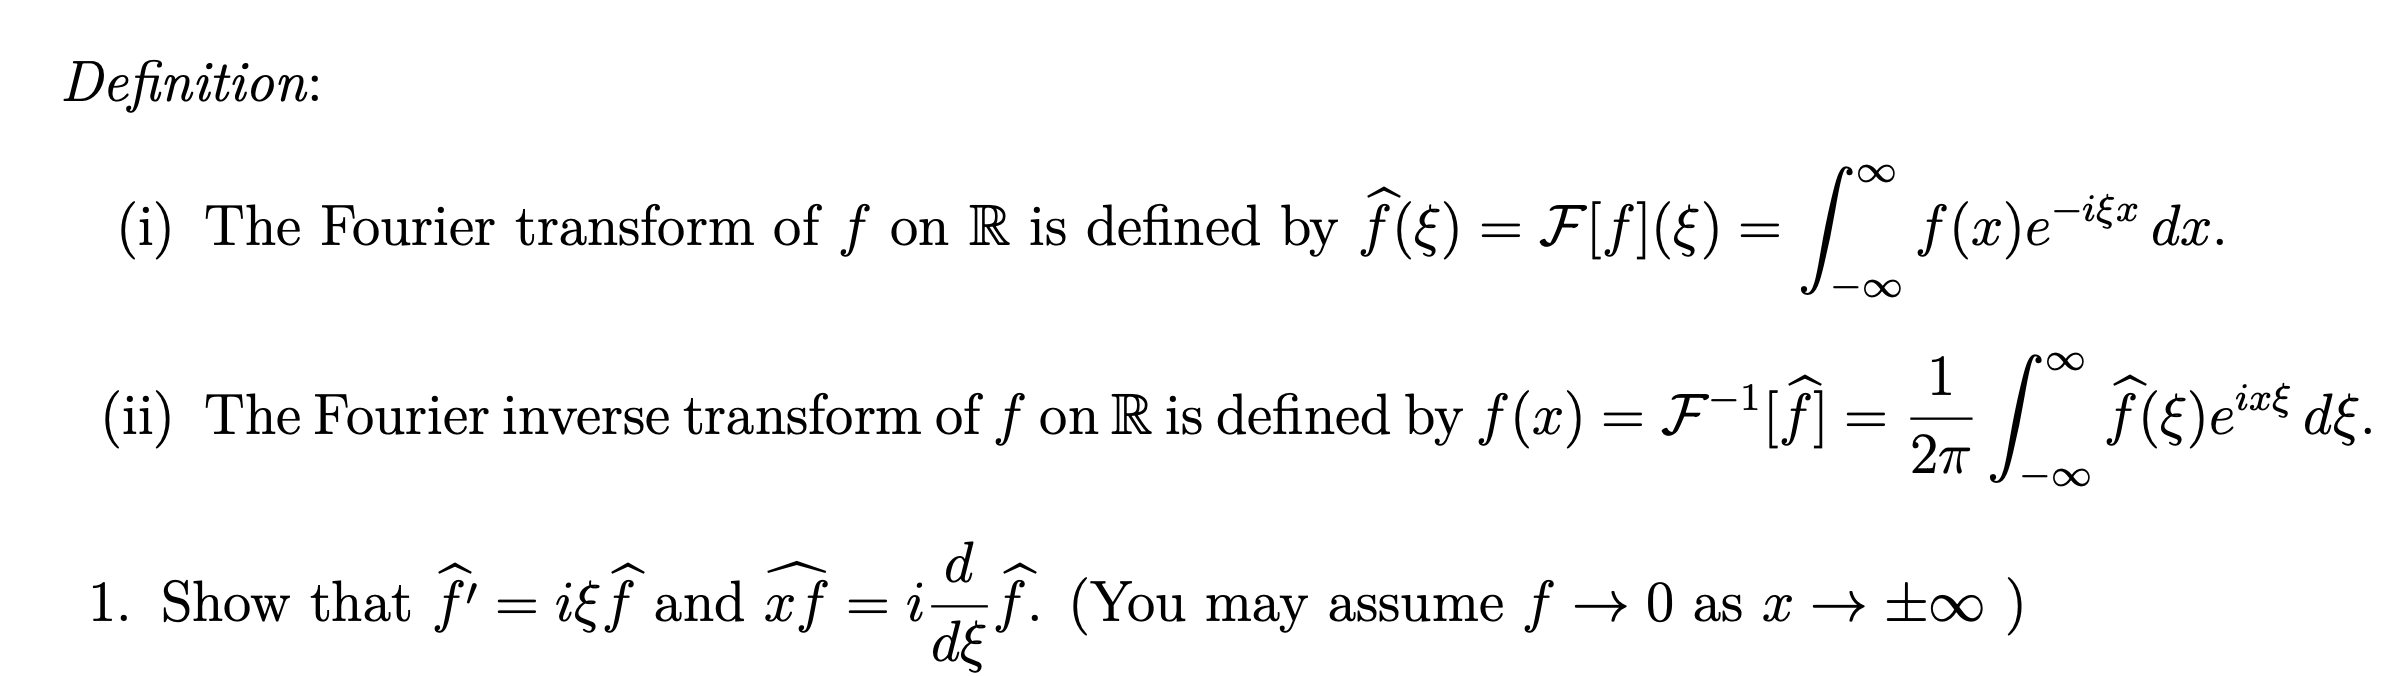
\includegraphics[height=6cm,width=18cm]{hw3q1}
\end{question}
\begin{proof}
Compute 
\begin{align*}
\hat{f'}-i\xi \hat{f}&=\int_{-\infty}^{\infty}\big( f'(x)e^{-i\xi x}-i\xi f(x)e^{-i \xi x}\big)dx\\
&=f(x)e^{-i\xi x}\Big|_{x=-\infty}^{\infty}
\end{align*}
Note that 
\begin{align*}
\abso{f(x)e^{-i\xi x}}= \abso{f(x)}
\end{align*}
Compute 
\begin{align*}
 \Big|f(M)e^{-i\xi M}-f(-M)e^{i \xi M} \Big|\leq  \abso{f(M)}+ \abso{f(-M)}\to 0\text{ as $M\to \infty$ }\\
\end{align*}
This now implies  
\begin{align*}
\hat{f'}-i \xi \hat{f}=\lim_{M\to \infty}f(x)e^{-i \xi x}\big|_{x=-M}^{M}=0
\end{align*}
Define 
 \begin{align*}
\phi(x,\xi)\triangleq f(x)e^{-i\xi x}
\end{align*}
It is clear that 
\begin{align*}
\partial_{\xi}\phi(x,\xi)=-ixf(x)e^{- i\xi x}\text{ is continuous every where }
\end{align*}
Then, we can apply Feynman's Trick to compute
\begin{align*}
i \frac{d}{d\xi}\hat{f}&= i \frac{d}{d\xi}\int_{-\infty}^{\infty}f(x)e^{-i\xi x}dx\\
&=i \int_{-\infty}^{\infty}-ix f(x)e^{-i\xi x}dx\\
&=\int_{-\infty}^{\infty}xf(x)e^{-i\xi x}dx=\widehat{xf}
\end{align*}
\end{proof}
\begin{theorem}
\label{Gau1} 
\textbf{(Gaussian Integral)} 
\begin{align*}
\int_{-\infty}^{\infty}e^{-x^2}dx=\sqrt{\pi} 
\end{align*}
\end{theorem}
\begin{proof}
Fix $I=\int_{-\infty}^{\infty}e^{-x^2}dx$. Compute using Fubini's Theorem 
\begin{align*}
I^2&=\int_{-\infty}^{\infty}e^{-x^2}dx\int_{-\infty}^{\infty}e^{-y^2}dy\\
&=\int_{-\infty}^{\infty}\int_{-\infty}^{\infty}e^{-(x^2+y^2)}dxdy\\
&=\int_0^{\infty}\int_{0}^{2\pi}re^{-r^2}d\theta dr\\
&=2\pi \int_0^{\infty}re^{-r^2}dr\\
&=-\pi e^{-r^2}\big|_{r=0}^{\infty}=\pi
\end{align*}
Because $e^{-x^2}$ is a positive function, we now have 
\begin{align*}
\int_{-\infty}^{\infty}e^{-x^2}dx=I=\sqrt{I^2}=\sqrt{\pi}  
\end{align*}
\end{proof}
\begin{theorem}
\label{Gau2}
\textbf{(Gaussian Integral)}
\begin{align*}
\int_{-\infty}^{\infty}e^{-\frac{(x-a)^2}{b}}dx
\end{align*}
\end{theorem}
\begin{proof}
Fix 
\begin{align*}
y\triangleq \frac{x-a}{\sqrt{b}}\text{ and }\frac{dy}{dx}=\frac{1}{\sqrt{b} }
\end{align*}
Compute using \myref{Theorem}{Gau1}
\begin{align*}
\int_{-\infty}^{\infty}e^{-\frac{(x-a)^2}{b}}dx&=\int_{-\infty}^{\infty}e^{-y^2}\sqrt{b} dy\\
&=\sqrt{b\pi} 
\end{align*}
\end{proof}
\begin{question}{}{}
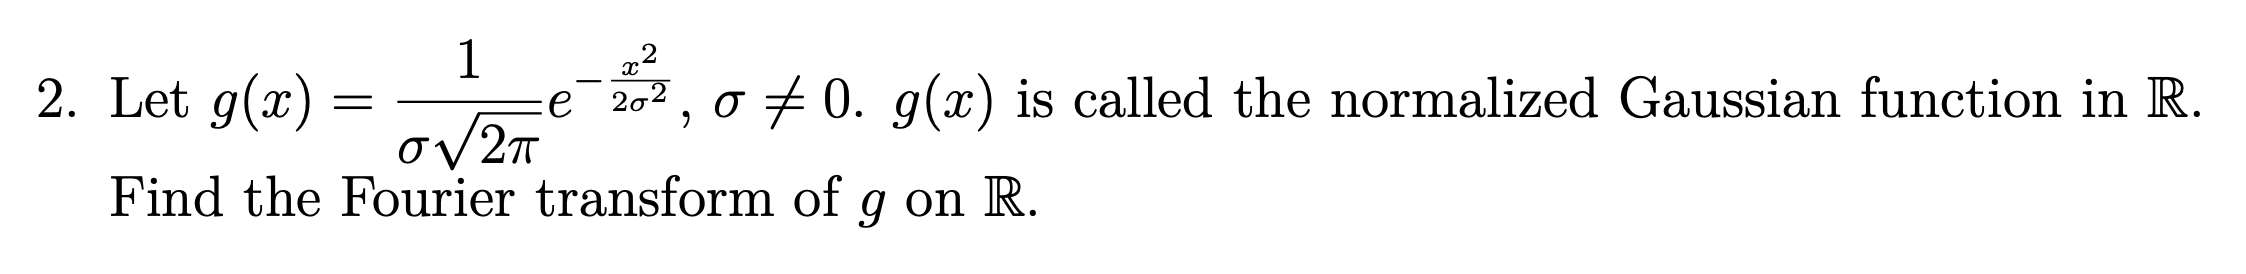
\includegraphics[height=3cm,width=18cm]{hw3q2}
\end{question}
\begin{proof}
Compute 
\begin{align*}
g'(x)=\frac{1}{\sigma \sqrt{2\pi} }\cdot \frac{-2x}{2\sigma^2}  e^{\frac{-x^2}{2\sigma^2}}= -\frac{1}{\sigma^2}xg(x)
\end{align*}
Using the statement of the first question, which we have proved, we now have 
\begin{align*}
  i \xi \widehat{g}= \widehat{g'} = - \frac{1}{\sigma^2} \widehat{xg} =  \frac{-i}{\sigma^2}  \frac{d\widehat{g}}{d\xi}
\end{align*}
This give us the first order homogenoeous ODE 
\begin{align*}
  \frac{d}{d\xi}\widehat{g}+ \sigma^2 \xi \widehat{g}=0
\end{align*}
Compute the general solution 
\begin{align*}
\widehat{g}(\xi)= C e^{\frac{-\sigma^2 \xi^2}{2}}
\end{align*}
Compute using \myref{Theorem}{Gau2}
\begin{align*}
C=\widehat{g}(0)=\int_{-\infty}^{\infty}g(x)dx=1
\end{align*}
We now have the $\underline{\text{answer}}$ 
\begin{align*}
\widehat{g}(\xi)=e^{\frac{-\sigma^2\xi^2}{2}}
\end{align*}
\end{proof}

\begin{question}{}{}
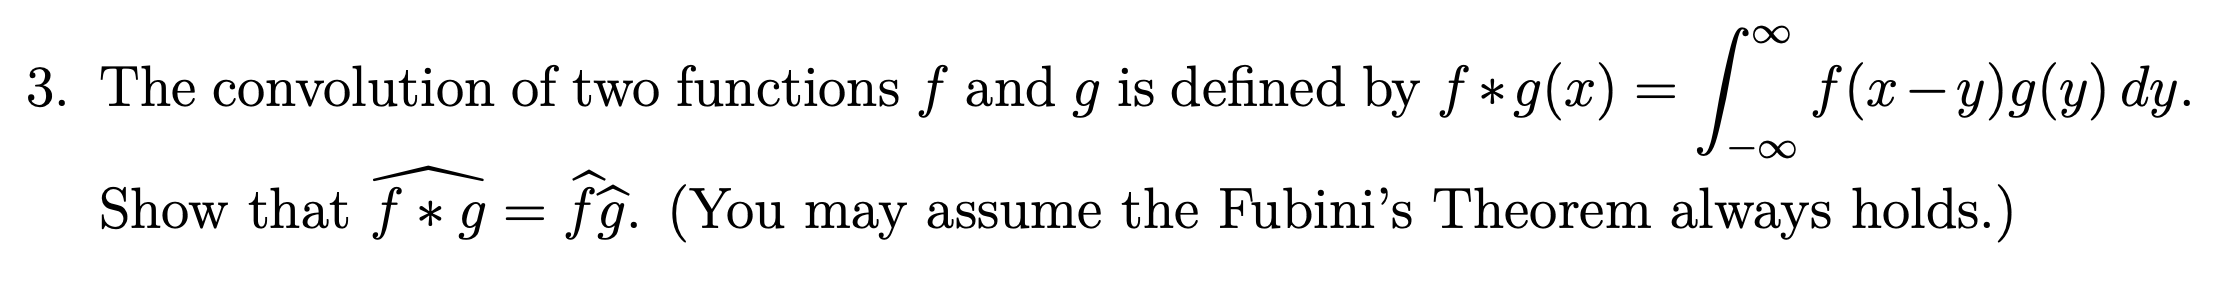
\includegraphics[height=3cm,width=18cm]{hw3q3}
\end{question}
\begin{proof}
Compute using Fubini's Theorem
\begin{align*}
  \widehat{f*g}(\xi)&=\int_{-\infty}^{\infty}(f*g)(u)e^{-i\xi u}du\\
  &=\int_{-\infty}^{\infty}\int_{-\infty}^{\infty}f(u-y)g(y)e^{-i\xi u}dudy
\end{align*}
Compute using Fubini's Theorem 
\begin{align*}
\widehat{f}\cdot \widehat{g}(\xi)&=\int_{-\infty}^{\infty}f(x)e^{-i\xi x}dx\int_{-\infty}^{\infty}g(y)e^{-\xi y}dy\\
&=\int_{-\infty}^{\infty}\int_{-\infty}^{\infty}f(x)g(y)e^{-i\xi (x+y)}dxdy\\
  &=\int_{-\infty}^{\infty}\int_{-\infty}^{\infty}f(u-y)g(y)e^{-i\xi u}dudy\hspace{0.5cm}\text{ where $u=x+y$ and  $\frac{du}{dx}=1$ }\\
  &=\widehat{f*g}(\xi)
\end{align*}
\end{proof}

\begin{question}{}{}
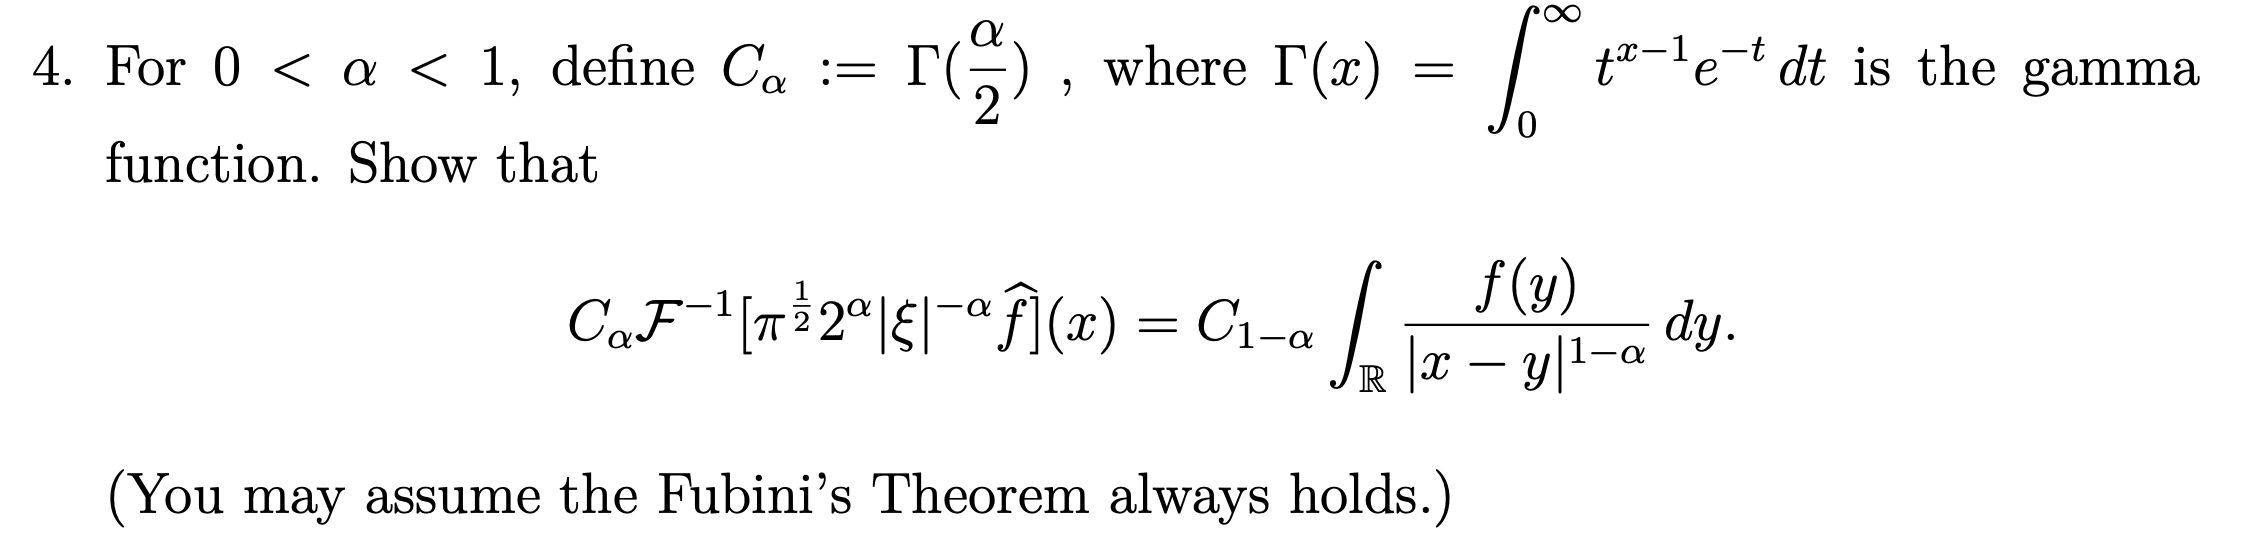
\includegraphics[height=5cm,width=18cm]{hw3q4}
\end{question}
\begin{proof}
Define 
\begin{align*}
g(x)\triangleq \frac{1}{\abso{x}^{1-\alpha }}
\end{align*}
We see 
\begin{align*}
\int_\R \frac{f(y)}{\abso{x-y}^{1-\alpha }}dy&=\int_\R \frac{f(x-u)}{\abso{u}^{1-\alpha }}du\hspace{0.3cm}(\because u=x-y)\\
&=\int_{\R} f(x-u)g(u)du=f*g(x)
\end{align*}
Compute 
\begin{align*}
C_{\alpha }\mathcal{F}^{-1}[\pi^{\frac{1}{2}}2^{\alpha }\abso{\xi}^{-\alpha }\widehat{f}](x)&=C_\alpha \pi^{\frac{1}{2}}2^{\alpha } \mathcal{F}^{-1}[\abso{\xi}^{-\alpha } \widehat{f}](x)
\end{align*}
We now can reduce the problem into proving 
\begin{align*}
\vi{C_\alpha \pi^{\frac{1}{2}}2^{\alpha } \mathcal{F}^{-1}[\abso{\xi}^{-\alpha } \widehat{f}](x)=C_{1-\alpha }f* g(x)}
\end{align*}
Using Fourier Inversion Theorem, and Convolution Theorem, we then can reduce the problem into proving  
\begin{align*}
  \vi{C_\alpha \pi^{\frac{1}{2}}2^{\alpha } \frac{1}{\abso{\xi}^{\alpha }} \widehat{f}(\xi)=C_{1-\alpha }\widehat{g}(\xi)\cdot \widehat{f}(\xi)}
\end{align*}
Then, we reduce the problem into 
\begin{align*}
\vi{C_\alpha \pi^{\frac{1}{2}}2^{\alpha }\frac{1}{\abso{\xi}^{\alpha }}=C_{1-\alpha }\widehat{g}(\xi)}
\end{align*}
Compute 
\begin{align*}
\widehat{g}(\xi)&=\int_{-\infty}^{\infty} \abso{x}^{\alpha -1}e^{-i \xi x}dx\\
&=\int_{-\infty}^{\infty} \abso{x}^{\alpha -1}\big(\cos (\xi x)- i \sin (\xi x) \big)dx\\
&=\int_{-\infty}^{\infty}\abso{x}^{\alpha -1}\cos (\xi x)dx\hspace{0.5cm}(\because \abso{x}^{\alpha -1}\sin (\xi x)\text{ is odd in $x$ })\\
&=2\int_{0}^{\infty}\abso{x}^{\alpha -1}\cos (\xi x)dx\hspace{0.5cm}(\because \abso{x}^{\alpha -1}\cos (\xi x)\text{ is even in $x$ })\\
&=2\int_{0}^{\infty}\abso{x}^{\alpha -1}\text{Re }e^{i \xi x}dx\\
&=\text{Re }2\int_{0}^{\infty}\abso{x}^{\alpha -1}e^{i \xi x}dx\\
&=\text{Re }2\int_{0}^{\infty} \abso{\frac{u}{\xi}}^{\alpha -1}e^{iu}\frac{du}{\xi}\hspace{0.5cm}( u\equiv\xi x)\\
&=\text{Re } \frac{2}{\abso{\xi}^{\alpha }}\int_0^{\infty}u^{\alpha -1}e^{iu}du\\
&=\text{Re }\frac{2}{\abso{\xi}^{\alpha }}e^{i \frac{\alpha \pi}{2}}\int_0^{\infty}x^{\alpha -1}e^{-x}dx\hspace{0.5cm}(\because \text{ Cauchy Integral Theorem })\\
&=\text{Re }\frac{2}{\abso{\xi}^{\alpha }}e^{i \frac{\alpha \pi}{2}}\Gamma(\alpha )\\
&=\frac{2\cos \frac{\alpha \pi}{2}\Gamma (\alpha )}{\abso{\xi}^{\alpha }}
\end{align*}
We can reduce our problem into proving 
\begin{align*}
  \vi{\frac{\Gamma (\frac{\alpha}{2})\sqrt{\pi} 2^{\alpha }}{\abso{\xi}^{\alpha }}=\frac{2\cos \frac{\alpha \pi}{2}\Gamma (\alpha )\Gamma (\frac{1-\alpha }{2})}{\abso{\xi}^{\alpha }}}
\end{align*}
Reduce to 
\begin{align*}
  \vi{\Gamma (\frac{\alpha }{2})\sqrt{\pi} 2^{\alpha -1}=\cos \frac{\alpha \pi}{2}\Gamma (\alpha )\Gamma (\frac{1-\alpha }{2})}
\end{align*}
Note that the Legendre Duplication Formula give us 
\begin{align*}
\Gamma (\frac{\alpha }{2})\Gamma (\frac{\alpha +1}{2})=2^{1-\alpha }\Gamma (\alpha )\sqrt{\pi} 
\end{align*}
This give us 
\begin{align}
\label{game1}
\Gamma (\frac{\alpha}{2})\sqrt{\pi}2^{\alpha -1}&= \frac{2^{1-\alpha }\Gamma (\alpha )\sqrt{\pi} }{\Gamma (\frac{\alpha +1}{2})}\sqrt{\pi} 2^{\alpha -1}\notag\\
&=\frac{\Gamma (\alpha )\pi }{\Gamma (\frac{\alpha +1}{2})}
\end{align}
Note that Euler Reflection Formula give us 
\begin{align*}
\Gamma (\frac{1-\alpha }{2})\Gamma (\frac{1+\alpha}{2})=\frac{\pi}{\sin (\pi \frac{1+\alpha }{2})}= \frac{\pi}{\cos \frac{\alpha \pi}{2}}
\end{align*}
This give us 
\begin{align}
  \label{game2}
\cos \frac{\alpha \pi}{2}\Gamma (\frac{1-\alpha }{2}) \Gamma (\alpha )&= \cos \frac{\alpha \pi}{2}\Gamma (\alpha )  \frac{\pi}{\cos \frac{\alpha \pi}{2}\Gamma  (\frac{1+\alpha }{2})}\notag\\
&=\frac{\Gamma (\alpha )\pi}{\Gamma (\frac{\alpha +1}{2})}
\end{align}
Note that \myref{Equation}{game1} and \myref{Equation}{game2} are identical, and we are done. $\vdone$
\end{proof}
\begin{theorem}
\label{6.5.2}
\textbf{(Remainder of Taylor's Theorem in Mean Values Form)} Given 
\begin{align*}
f:I\subseteq \R\rightarrow \R\text{ is $n$ time continuously differentiable at $a\in I$}
\end{align*}
Define 
\begin{enumerate}[label=(\alph*)]
  \item $P_n(x)\triangleq \sum_{k=0}^n \frac{f^{(k)}(a) (x-a)^k}{k!}$ 
  \item  $R_n(x)\triangleq f(x)-P_n(x)$
\end{enumerate}
If 
\begin{enumerate}[label=(\alph*)]
  \item $G$ is continuous on  $[a,x]$ 
  \item  $G'$ exists and not equals to  $0$ on  $(a,x)$
\end{enumerate}
We have 
\begin{align*}
\exists \xi \in (a,x), R_n(x)=\frac{f^{(n+1)}(\xi)(x-\xi )^n}{n!}  \frac{G(x)-G(a)}{G'(\xi )}
\end{align*}
\end{theorem}
\begin{proof}
WLOG suppose $x>a$. Define $F:(a,x)\to \R$ by 
\begin{align*}
F(t)=\sum_{k=0}^n \frac{f^{(k)}(t)(x-t)^k}{k!}
\end{align*}
By Cauchy's MVT, we know  
\begin{align*}
\exists \xi\in (a,x),\frac{F'(\xi)}{G'(\xi)}=\frac{F(x)-F(a)}{G(x)-G(a)}
\end{align*}
Compute 
\begin{align*}
F(x)=f(x)
\end{align*}
Compute 
\begin{align*}
F(a)=\sum_{k=0}^n \frac{f^{(k)}(a)(x-a)^k}{k!}=P_n(x)
\end{align*}
Compute 
\begin{align*}
F'(\xi)&=\sum_{k=0}^n \frac{f^{(k+1)}(\xi)(x-\xi)^k-k f^{(k)}(\xi)(x-\xi)^{k-1}}{k!}\\
&=\frac{f^{(n+1)}(\xi)(x-\xi)^n}{n!} 
\end{align*}
We now have 
\begin{align*}
\frac{\frac{f^{(n+1)}(\xi)(x-\xi)^{n}}{n!}}{G'(\xi)}=\frac{R_n(x)}{G(x)-G(a)}
\end{align*}
Then we can deduce 
\begin{align*}
R_n(x)=\frac{f^{(n+1)}(\xi)(x-\xi)^n}{n!}\frac{G(x)-G(a)}{G'(\xi)}
\end{align*}
\end{proof}
\begin{corollary}
\label{6.5.3}
\textbf{(Lagarange Form of Remainders in Taylor's Theorem)} Let 
\begin{align*}
G(t)=(x-t)^{n+1}
\end{align*}
We have
\begin{align*}
\exists \xi \in (a,x), R_n(x)=\frac{f^{(n+1)}(\xi)(x-a)^{n+1}}{(n+1)!} 
\end{align*}
\end{corollary}
\begin{proof}
Compute 
\begin{align*}
G'(\xi)&=-(n+1)(x-\xi)^{n}\\
G(x)&=0\\
G(a)&=(x-a)^{n+1}
\end{align*}
The result now follows from \myref{Theorem}{6.5.2}. 
\end{proof}
\begin{theorem}
\label{sinxx}
\textbf{($\sin x\leq x$)}
\begin{align*}
\hspace{2cm}\abso{\sin x}\leq \abso{x}\hspace{1.5cm}(x\in [\frac{-\pi}{2},\frac{\pi}{2}])
\end{align*}
\end{theorem}
\begin{proof}
Because $\abso{\sin x}$ and $\abso{x}$ are both odd and positive, WOLG, we only have to prove when $x\in (0,\frac{\pi}{2}]$. Compute the Taylor polynomials to second degree and its remainder. 
\begin{align*}
\sin x= x- \cos (\xi)\frac{x^3}{3!}\text{ for some $\xi\in (0,x)$  }
\end{align*}
Because $0<\xi <x$, it is now clear that 
\begin{align*}
0< \sin x =x- \cos(\xi) \frac{x^3}{3!}\leq x
\end{align*}
This then implies 
\begin{align*}
\abso{\sin x}\leq \abso{x}
\end{align*}
\end{proof}
\begin{question}{}{}
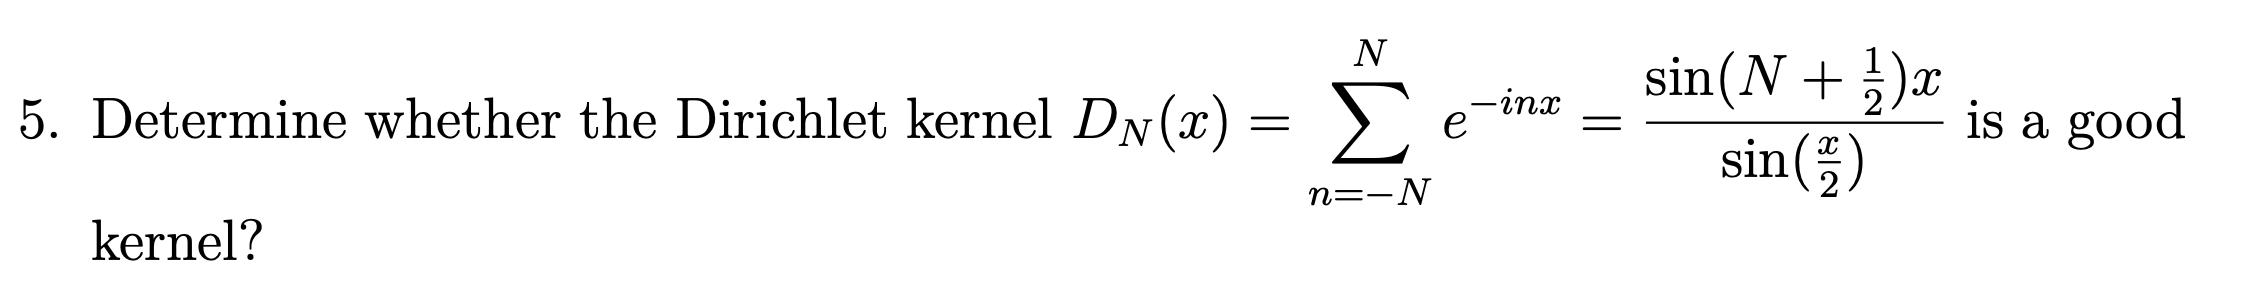
\includegraphics[height=3cm,width=18cm]{hw3q5}
\end{question}
\begin{proof}
No. Compute using \myref{Theorem}{sinxx}
\begin{align*}
\int_{-\pi}^{\pi}\abso{D_N(x)}dx&=\int_{-\pi}^{\pi}\abso{\frac{\sin (N+\frac{1}{2})x}{\sin (\frac{x}{2})}}dx\\
&\geq 2\int_{-\pi}^{\pi} \frac{\abso{\sin (N+\frac{1}{2})x}}{\abso{x}}dx
\end{align*}
Using $u=(N+\frac{1}{2})x,dx=\frac{du}{N+\frac{1}{2}}$, we have the approximation
\begin{align*}
  2\int_{-(N+\frac{1}{2})\pi}^{(N+\frac{1}{2})\pi} \frac{\abso{\sin u}}{\abso{\frac{u}{N+\frac{1}{2}}}}\frac{1}{N+\frac{1}{2}}du&=4\int_{0}^{(N+\frac{1}{2})\pi} \frac{\abso{\sin u}}{\abso{u}}du\\
&\geq 4\Big(\int_0^{\pi}\frac{\sin u}{u}du+\int_{\pi}^{N\pi} \frac{\abso{\sin u} }{\abso{u} }du+\int_{N\pi}^{(N+\frac{1}{2})\pi} \frac{\abso{\sin u}}{\abso{u}}du \Big)\\
&\geq 4\Big(\int_0^{\pi}\frac{\sin u}{\pi}du+\int_{\pi}^{N\pi} \frac{\abso{\sin u} }{\abso{u} }du+\int_{N\pi}^{(N+\frac{1}{2})\pi} \frac{\abso{\sin u}}{(N+\frac{1}{2})\pi}du \Big)\\
&= 4\int_{\pi}^{N\pi} \frac{\abso{\sin u}}{\abso{u}}du+\frac{8}{\pi}+\frac{4}{(N+\frac{1}{2})\pi} \\
&=4\sum_{k=1}^{N-1}\int_{k\pi}^{(k+1)\pi } \frac{\abso{\sin u}}{\abso{u}}du+\frac{8}{\pi}+\frac{4}{(N+\frac{1}{2})\pi}\\
&\geq 4 \sum_{k=1}^{N-1}\frac{1}{(k+1)\pi} \int_{k\pi}^{(k+1)\pi} \abso{\sin u}du+\frac{8}{\pi}+\frac{4}{(N +\frac{1}{2})\pi}\\
&=4\sum_{k=1}^{N-1}\frac{2}{(k+1)\pi}+\frac{8}{\pi}+\frac{4}{(N+\frac{1}{2})\pi}\\
&=\frac{8}{\pi}\sum_{k=1}^{N-1}\frac{1}{k+1}+\frac{8}{\pi}+\frac{4}{(N+\frac{1}{2})\pi}\to \infty
\end{align*}
where the last expression tends to infinity because $\sum_{k=1}^{N}\frac{1}{k}$ tends to infinity and the other two terms stay bounded.\\

We have now seen 
\begin{align*}
  \int_{-\pi}^{\pi}\abso{D_N(x)}dx&\geq 2\int_{-\pi}^{\pi} \frac{\abso{\sin (N+\frac{1}{2})x}}{\abso{x}}dx\\
  &= 2\int_{-(N+\frac{1}{2})\pi}^{(N+\frac{1}{2})\pi} \frac{\abso{\sin u}}{\abso{\frac{u}{N+\frac{1}{2}}}}\frac{1}{N+\frac{1}{2}}du \to \infty\text{ as }N\to \infty
\end{align*}
This shows that the Dirichlet's Kernel $D_N(x)$ does NOT satisfy the second criterion. 
\end{proof}



\begin{lemma}
\label{Dkernel variant}
\begin{align*}
D_N(x)\triangleq \sum_{n=-N}^{N}e^{-inx}=1+2\sum_{n=1}^N \cos nx = \frac{\sin (N+\frac{1}{2})x}{\sin \frac{x}{2}}
\end{align*}
\end{lemma}
\begin{proof}
\begin{align*}
\sum_{n=-N}^{N}e^{-i nx}&=1+2\sum_{n=1}^N \big(\cos nx+ i \sin nx + \cos nx - i \sin nx \big)\\
&=1+2\sum_{n=1}^N \cos nx
\end{align*}
\end{proof}
\begin{lemma}
\label{sinx/2}
\begin{align*}
\hspace{3cm}\abso{\sin x}\geq \frac{\abso{x}}{2}\hspace{1.5cm}(x\in  [-\frac{\pi}{2},\frac{\pi}{2}] )
\end{align*}
\end{lemma}
\begin{proof}
Because both $\abso{\sin x}\text{ and }\frac{\abso{x}}{2}$ are both odd and positive, WOLG, it suffices to just prove  for $x \in (0,\frac{\pi}{2}]$.\\

Notice that $\sin x$ is concave on $[0,\frac{\pi}{2}]$ by computing second derivative.\\

Then, for all $x\in [0,\frac{\pi}{2}]$, we have
\begin{align*}
\sin x \geq \sin 0+ x \frac{\sin \frac{\pi}{2}- \sin 0}{\frac{\pi}{2}-0}
\end{align*}
This give us 
\begin{align*}
\sin x\geq \frac{2x}{\pi}\geq \frac{x}{2}\hspace{0.5cm}(\because 2\geq  \frac{\pi}{2} )
\end{align*}
\end{proof}
\begin{question}{}{}
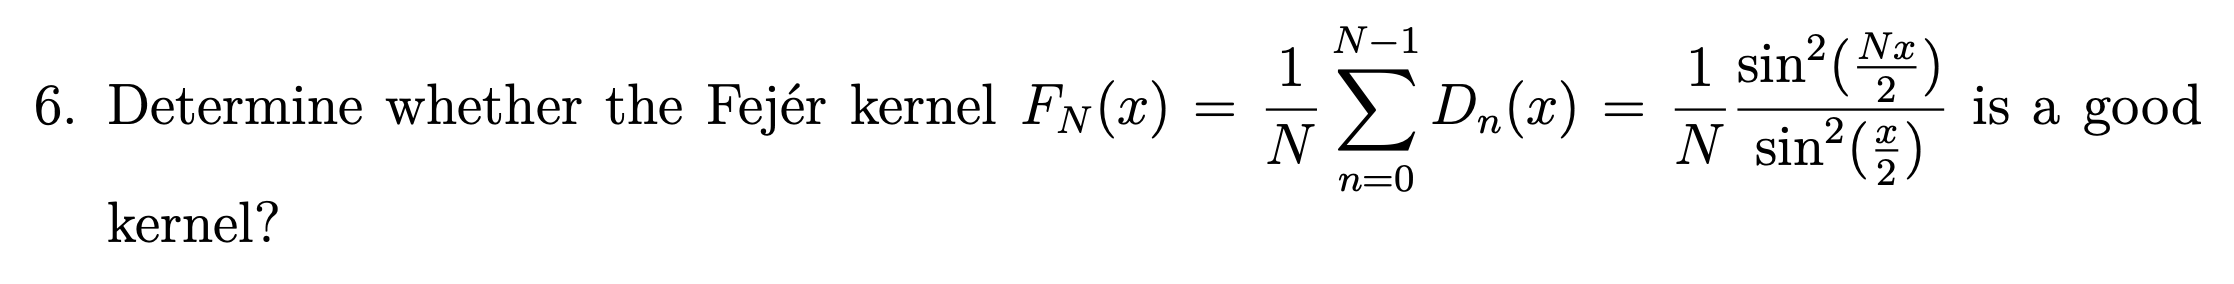
\includegraphics[height=3cm,width=18cm]{hw3q6}
\end{question}
\begin{proof}
Yes. For first condition, compute 
\begin{align*}
\frac{1}{2\pi}\int_{-\pi}^\pi F_N(x)dx&=\frac{1}{2\pi}\int_{-\pi}^{\pi} \frac{1}{N+1}\sum_{n=0}^N \frac{\sin (n+\frac{1}{2})x}{\sin \frac{x}{2}}dx\\
&=\frac{1}{2\pi (N+1)}\sum_{n=0}^N \int_{-\pi}^{\pi} D_n(x)dx\\
&=\frac{1}{2\pi (N+1)}\sum_{n=0}^N \int_{-\pi}^{\pi} (1+2 \sum_{k=1}^n \cos kx)dx\hspace{0.5cm}(\text{\myref{Lemma}{Dkernel variant}})\\
&=\frac{1}{2\pi(N+1)}\sum_{n=0}^N 2\pi=1\hspace{0.5cm}(\because \int_{-\pi}^{\pi}\cos kx=0)
\end{align*}
For second condition, just not that $F_N$ is positive, so 
\begin{align*}
\int_{-\pi}^{\pi}\abso{F_n(x)}dx=\int_{-\pi}^{\pi}F_n(x)=2\pi
\end{align*}
For third condition, suppose $0<\delta \leq \abso{x}\leq \pi$.\\

Using \myref{Lemma}{sinx/2} to compute 
\begin{align*}
0\leq F_n(x)&=\frac{\sin^2 \frac{nx}{2}}{n \sin^2 \frac{x}{2}}\leq \frac{1}{n \sin^2 \frac{x}{2}}\leq \frac{1}{n(\frac{x}{4})^2}\leq \frac{1}{n(\frac{\delta}{4})^2}\searrow 0\text{ as $n\to \infty$ }
\end{align*}
Then 
\begin{align*}
\int_{\delta\leq \abso{x}\leq \pi}F_n(x)dx\leq \int_{\delta\leq \abso{x}\leq \pi} \frac{16}{n\delta^2}dx=\frac{32(\pi-\delta)}{n \delta^2}\searrow 0\text{ as $n\to \infty$ }
\end{align*}


\end{proof}

\begin{question}{}{}
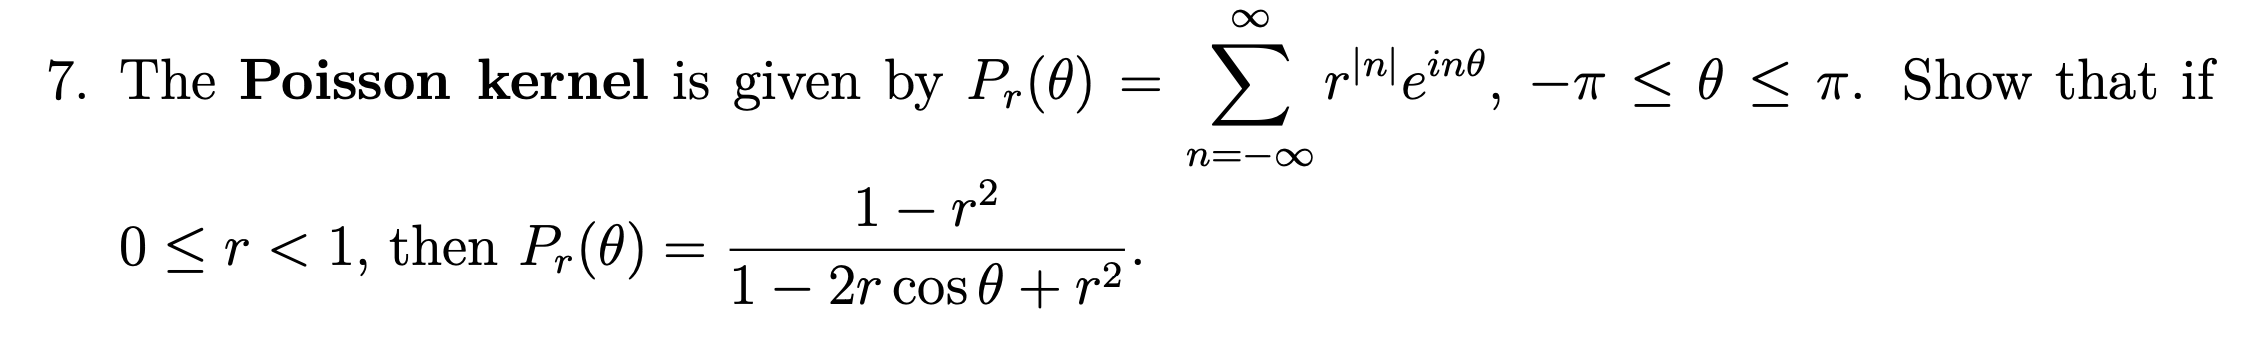
\includegraphics[height=3cm,width=18cm]{hw3q7}
\end{question}
\begin{proof}
Compute 
\begin{align*}
P_r(\theta)&=\sum_{n=-\infty}^{\infty}r^{\abso{n}}e^{i n\theta}\\
&=1+\sum_{n=1}^{\infty}r^n e^{i n\theta} + \sum_{n=1}^{\infty}r^n e^{-i n \theta}\\
&=1+\frac{re^{i\theta}}{1-re^{i\theta}}+\frac{re^{-i\theta}}{1-re^{-i \theta}}\\
&=1+ \frac{re^{i\theta}(1-re^{-i\theta})+re^{-i\theta}(1-re^{i\theta})}{(1-re^{i\theta})(1-re^{-i \theta})}\\
&=1+ \frac{re^{i\theta}+re^{-i\theta}-2r^2}{1-re^{i\theta}-re^{-i\theta}+r^2}\\
&=1+\frac{2r\cos \theta-2r^2}{1-2r\cos \theta+r^2}=\frac{1-r^2}{1-2r\cos \theta +r^2}
\end{align*}
\end{proof}


\begin{question}{}{}
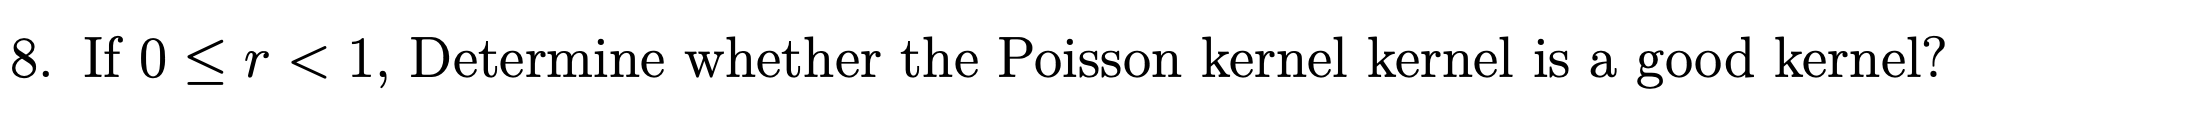
\includegraphics[height=2cm,width=18cm]{hw3q8}
\end{question}
\begin{proof}
Yes. For first condition, compute 
\begin{align*}
\frac{1}{2\pi}\int_{-\pi}^{\pi} P_r(\theta)d\theta &=\frac{1}{2\pi}\int_{-\pi}^{\pi}\sum_{n=-\infty}^{\infty}r^{\abso{n}}e^{i n\theta}d\theta\\
&=\frac{1}{2\pi}\sum_{n=-\infty}^{\infty}r^{\abso{n}}\int_{-\pi}^{\pi}e^{i n \theta}d\theta\\
&=\frac{1}{2\pi}r^0 2\pi=1
\end{align*}
For second condition, note that 
\begin{align*}
1-2r \cos \theta+r^2\geq 1-2r+r^2=(1-r)^2\inr^+
\end{align*}
Then because $1-r^2\inr^+$, we see 
\begin{align*}
P_r(\theta)=\frac{1-r^2}{1-2r\cos \theta+r^2}\inr^+
\end{align*}
We now have 
\begin{align*}
  \int_{-\pi}^{\pi}\abso{P_r(\theta)}d\theta &=\int_{-\pi}^{\pi}P_r(\theta)d\theta=1
\end{align*}
Note that $P_r$ is even, we then can reduce proving the third critirion into proving 
\begin{align*}
\vi{P_r(\theta)\to 0\text{ uniformly on $[\delta,\pi]$ as $r\nearrow 1$ }}
\end{align*}
Compute 
\begin{align*}
P_r'(\theta)=\frac{-2r \sin \theta (1-r^2)}{(1-2r \cos \theta + r^2)^2}<0\text{ on $[\delta,\pi]$ }
\end{align*}
This then give us 
\begin{align*}
P_r(\theta)\leq P_r(\delta)\text{ on }[\delta,\pi]
\end{align*}
Compute 
\begin{align*}
P_r(\delta)=\frac{1-r^2}{(1-r)^2+2r(1-\cos \delta)}\to 0\text{ as $r\nearrow 1$ }
\end{align*}
and we are done $\vdone$
\end{proof}
\section{HW4}

\begin{question}{}{}
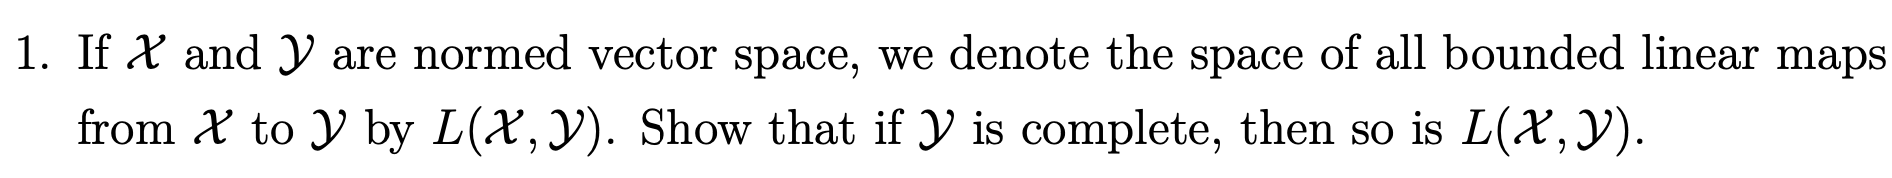
\includegraphics[height=3cm,width=18cm]{ahw4q1}
\end{question}
\begin{proof}
Suppose $\mathcal{Y}$ is complete. Let $BL(\mathcal{X},\mathcal{Y})$ be the space of bounded linear transformation from $\mathcal{X}$ to $\mathcal{Y}$. We wish to prove 
 \begin{align*}
\vi{\Big(BL(\mathcal{X},\mathcal{Y}),\norm{\cdot}_{\text{op}} \Big)\text{ is complete }}
\end{align*}
Fix a Cauchy-sequence $\set{T_n}_{n\inn}$ in $\Big(BL(\mathcal{X},\mathcal{Y}),\norm{\cdot}_{\text{op}} \Big)$. We reduce the problem into proving 
\begin{align*}
\vi{\text{ $T_n$ converge to some bounded linear operator with respect to $\norm{\cdot}_\text{op}$ }}
\end{align*}
We first show 
\begin{align*}
\olive{\text{ for all $x\in \mathcal{X}$, the sequence $\set{T_nx}_{n\inn}$ converge in $\mathcal{Y}$}}
\end{align*}
Fix $x$. Because $\mathcal{Y}$ is complete, we can reduce the problem into showing 
\begin{align*}
\olive{\set{T_nx}_{n\inn}\text{ is Cauchy }}
\end{align*}
Fix $\epsilon $. We wish 
\begin{align*}
\olive{\text{ to find }N\text{ such that for all $n>m>N$ we have }\norm{T_nx-T_mx}_{\mathcal{Y}}\leq \epsilon }
\end{align*}
Because  $\set{T_n}_{n\inn}$ is a Cauchy-sequence in $\Big(BL(\mathcal{X},\mathcal{Y}),\norm{\cdot}_{\text{op}} \Big)$, we know there exists $N'$ such that 
\begin{align*}
\norm{T_n-T_m}_{\text{op}}< \frac{\epsilon }{\norm{x}_{\mathcal{X}}} \text{ for all $n>m>N'$ }
\end{align*}
Note that if $\norm{x}_{\mathcal{X}}=0$, then $x=0$ and the proof become trivial.\\

We claim 
\begin{align*}
\olive{\text{ such }N'\text{ works }}
\end{align*}
Observe 
\begin{align*}
\norm{T_nx-T_mx}_\mathcal{Y}&=\norm{(T_n-T_m)x}_{\mathcal{Y}}\\
&\leq \norm{T_n-T_m}_{\text{op}} \norm{x}_{\mathcal{X}}< \epsilon \odone
\end{align*}
Now, we can define a function $S:\mathcal{X}\rightarrow \mathcal{Y}$ by 
\begin{align*}
S(x)\triangleq \lim_{n\to \infty}T_n(x)
\end{align*}
We claim 
\begin{align*}
\vi{S \in BL(\mathcal{X},\mathcal{Y})\text{ and }T_n \to S\text{ with respect to $\norm{\cdot}_\text{op}$ }}
\end{align*}
Observe 
\begin{align*}
S(x+cy)&=\lim_{n\to \infty}T_n(x+cy)\\
&=\lim_{n\to \infty}T_n(x)+cT_n(y)\\
&=\lim_{n\to \infty}T_n(x)+c\lim_{n\to \infty}T_n(y)=S(x)+cS(y)
\end{align*}
This show $S$ is indeed linear. Now, we show 
\begin{align*}
\blue{S\text{ is indeed bounded }}
\end{align*}
In other words, we wish to show 
\begin{align*}
  \blue{\set{\norm{Sx}_{\mathcal{Y}}: x \in \mathcal{X}\text{ and }\norm{x}_{\mathcal{X}}=1}\text{ is bounded  }}
\end{align*}
Because $T_n$ is Cauchy with respect to $\norm{\cdot}_{\text{op}}$, we know $\set{\norm{T_n}_\text{op}}$ is bounded by some $M\inr^+$. We claim 
\begin{align*}
\blue{\sup_{\norm{x}_{\mathcal{X}}=1} \norm{Sx}_{\mathcal{Y}}\leq M+1}
\end{align*}
Fix $\norm{x}_{\mathcal{X}}=1$. We reduce the problem into proving  
\begin{align*}
  \blue{\norm{Sx}_{\mathcal{Y}}\leq M+1}
\end{align*}
Because $T_nx \to Sx$ by definition of $S$, we know there exists some  $k\inn$ such that $\norm{T_kx-Sx}_{\mathcal{Y}}<1$. Now, observe 
\begin{align*}
  \norm{Sx}_\mathcal{Y}&\leq \norm{(S-T_k)x}_{\mathcal{Y}}+\norm{T_k(x)}_\mathcal{Y}\\
&<1+\norm{T_k}_{\text{op}}\hspace{0.5cm}(\because \norm{x}_{\mathcal{X}}=1)\\
&\leq 1+M \bdone
\end{align*}
It remains to prove 
\begin{align*}
  \vi{\norm{T_n-S}_{\text{op}}\to 0\text{ as }n\to \infty}
\end{align*}
Fix $\epsilon $. We wish 
\begin{align*}
\vi{\text{ to find $N$ such that for all $n>N$ we have }\norm{T_n-S}_\text{op}\leq \epsilon }
\end{align*}
Because $T_n$ is Cauchy with respect to $\norm{\cdot}_\text{op}$, we know there exists $N'$ such that for all $m>n>N'$, we have 
 \begin{align*}
\norm{T_m-T_n}_\text{op}<\epsilon 
\end{align*}
We claim 
\begin{align*}
\vi{\text{ such $N'$ works }}
\end{align*}
Fix $\norm{x}_{\mathcal{X}}=1$ and $n>N'$. We reduce the problem into proving 
 \begin{align*}
   \vi{\norm{T_n(x)-S(x)}_{\mathcal{Y}}\leq \epsilon }
\end{align*}
Observe 
\begin{align*}
\norm{T_n(x)-S(x)}_\mathcal{Y}&=\norm{T_n(x)-\lim_{m\to \infty}T_m(x)}_\mathcal{Y}\\
&=\norm{\lim_{m\to \infty}\big((T_n-T_m)(x)\big)}_{\mathcal{Y}}\\
&=\lim_{m\to \infty} \norm{(T_n-T_m)(x)}_{\mathcal{Y}}\hspace{0.5cm}(\because \text{ $\lim_{m\to \infty}\big((T_n-T_m)(x)\big)=T_n(x)-S(x)\text{ exists }$ })\\
&\leq \limsup_{m\to\infty} \norm{T_n-T_m}_\text{op} \leq \epsilon \vdone
\end{align*}





\end{proof}
\begin{question}{}{}
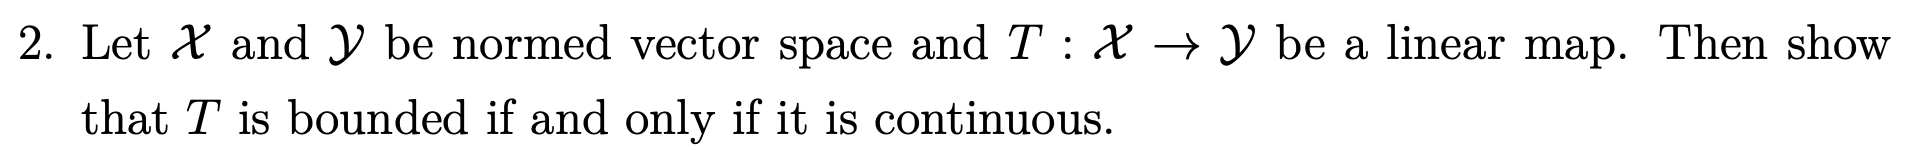
\includegraphics[height=3cm,width=18cm]{ahw4q2}
\end{question}
\begin{proof}
See \myref{Theorem}{LOB}
\end{proof}
\begin{question}{}{}
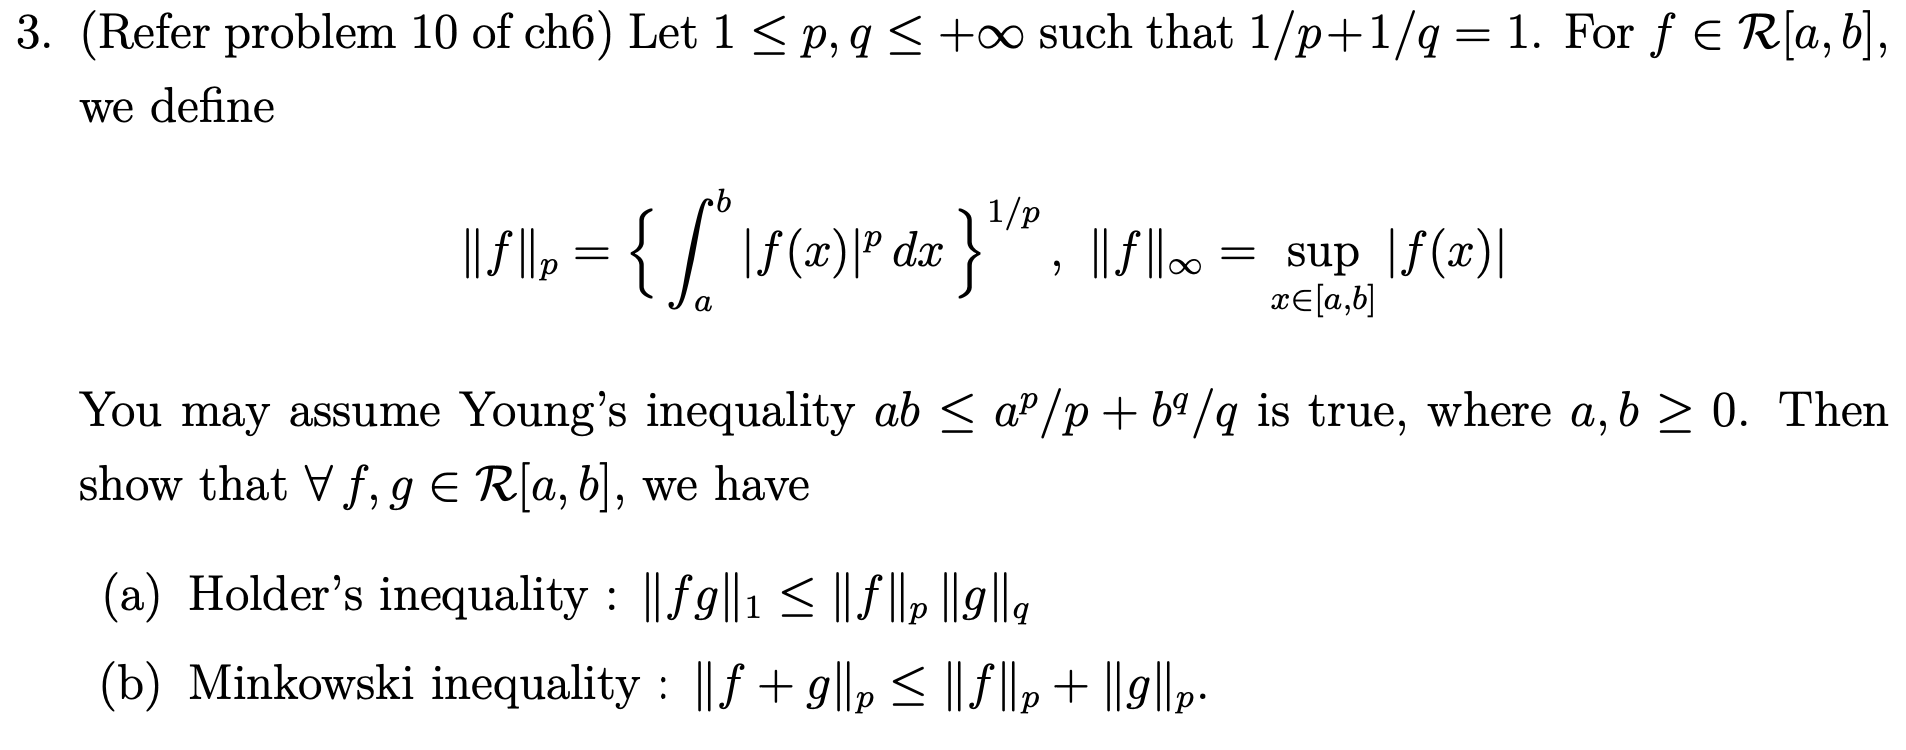
\includegraphics[height=8cm,width=18cm]{ahw4q3}
\end{question}
\begin{proof}
\textbf{(Proof of Holder's Inequality)}\\

We first prove 
\begin{align*}
\vi{\text{ when }p=1\text{ and when }q=1}
\end{align*}
WOLG, we 
\begin{align*}
\vi{\text{ only have to prove when }p=1}
\end{align*}
Because $\abso{g(x)}\leq \sup_{t\in [a,b]}\abso{g(t)}$ for all $x\in [a,b]$, we have
\begin{align*}
\int_a^b \abso{fg}dx\leq \int_a^b \abso{f}\sup_{t\in [a,b]}\abso{g(t)}dx=\norm{f}_1 \cdot \norm{g}_{\infty}\vdone
\end{align*}
We now prove 
\begin{align*}
\blue{\text{ when }p\in  (1,\infty)}
\end{align*}
We first prove 
\begin{align*}
  \brown{\text{ the special case $\norm{f}_p=0\text{ or }\norm{g}_q=0$ }}
\end{align*}
WOLG, suppose $\norm{f}_p=0$. From $\norm{f}_p=0$, we can deduce
\begin{align*}
\int_a^b \abso{f}^p dx=0
\end{align*}
This tell us $\abso{f}$ is $0$ almost everywhere, and give us 
\begin{align*}
\norm{fg}_1=\int_a^b \abso{fg}dx=0=\norm{f}_p\norm{g}_q\brown{\text{(done)}}
\end{align*}
Now, we come back 
\begin{align*}
\blue{\text{ to prove the general case where $\norm{f}_p\neq 0\neq \norm{g}_q$}}
\end{align*}
Applying young's inequality to $\frac{\abso{f}}{\norm{f}_p}$ and $\frac{\abso{g}}{\norm{g}_q}$, we have 
\begin{align*}
\frac{\abso{fg}}{\norm{f}_p\norm{g}_q}\leq \frac{1}{p}(\frac{\abso{f}}{\norm{f}_p})^p+\frac{1}{q}(\frac{\abso{g}}{\norm{g}_q})^q
\end{align*}
Integrating both side 
\begin{align*} \frac{1}{\norm{f}_p\norm{g}_q} \int_a^b \abso{fg}dx&\leq \frac{1}{p\norm{f}_p^p}\int_a^b \abso{f}^pdx + \frac{1}{q\norm{g}_q^q} \int_a^b \abso{g}^qdx \\
  &=\frac{1}{p\norm{f}_p^p}\norm{f}_p^p+\frac{1}{q\norm{g}_q^q}\norm{g}_q^q\\
  &=\frac{1}{p}+\frac{1}{q}=1
\end{align*}
Multiplying $\norm{f}_p\norm{g}_q$ to both side, we now have 
\begin{align*}
\norm{fg}_1=\int_a^b \abso{fg}dx\leq \norm{f}_p\norm{g}_q\bdone
\end{align*}
\textbf{(Proof of Minkowski inequality)}
Compute $\norm{f+g}_p^p$
\begin{align*}
\norm{f+g}_p^p&=\int_a^b \abso{f+g}^p dx\\
&\leq \int_a^b \abso{f+g}^{p-1} (\abso{f}+\abso{g})dx\\
&=\int_a^b \abso{f+g}^{p-1}\cdot \abso{f}dx+\int_a^b \abso{f+g}^{p-1}\cdot \abso{g}dx\\
&=\norm{\abso{f+g}^{p-1}f}_{1}+ \norm{\abso{f+g}^{p-1}g}_1
\end{align*}
Check that $\frac{p}{p-1}\text{ and }p$ form a holder conjugate. Now use Holder's Inequality 
\begin{align*}
  \norm{f+g}_p^p & \leq \norm{\abso{f+g}^{p-1}f}_{1}+ \norm{\abso{f+g}^{p-1}g}_1\\
  &\leq \norm{\abso{f+g}^{p-1}}_{\frac{p}{p-1}} \norm{f}_p+ \norm{\abso{f+g}}_{\frac{p}{p-1}} \norm{g}_p\\
  &=(\int_a^b \abso{f+g}^p dx)^{\frac{p-1}{p}}(\norm{f}_p+\norm{g}_p)\\
  &=\norm{f+g}_p^{p-1}(\norm{f}_p+\norm{g}_p)
\end{align*}
Dividing both side by $\norm{f+g}_p^{p-1}$ (note that if $\norm{f+g}_p^{p-1}=0$, then the proof become trivial),  
\begin{align*}
\norm{f+g}_p\leq \norm{f}_p+ \norm{g}_p
\end{align*}



\end{proof}
\begin{question}{}{}
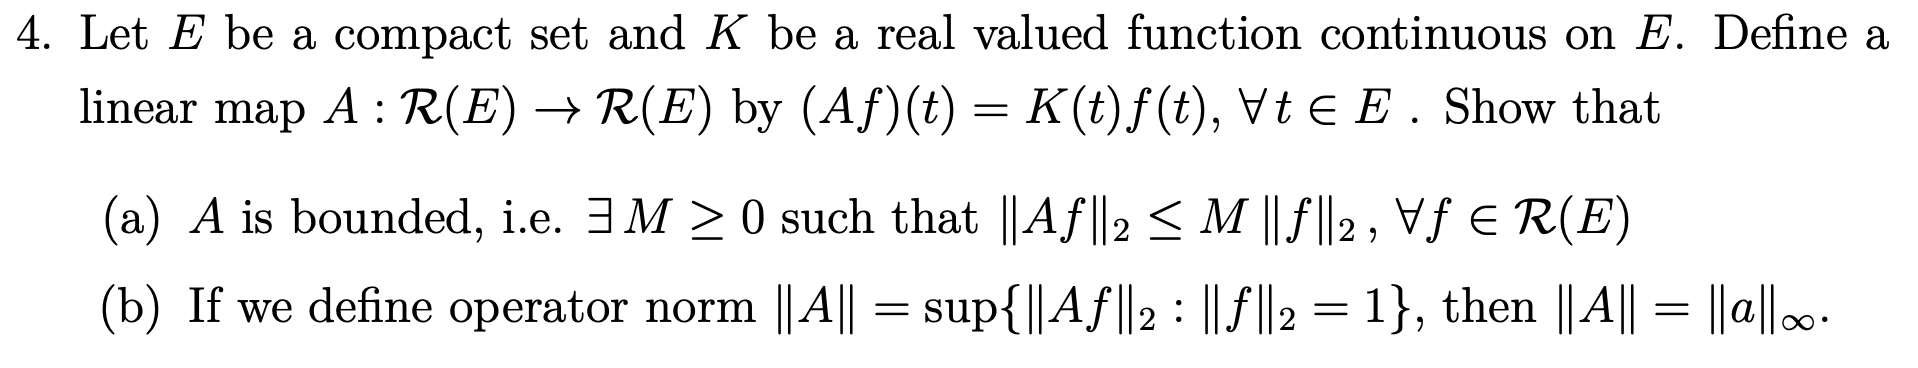
\includegraphics[height=5cm,width=18cm]{ahw4q4}
\end{question}
\begin{proof}
\textbf{(a)}\\

Because $E$ is compact and $K$ is continuous on $E$, we know
 \begin{align*}
M'=\sup_E \abso{K}^2\text{ exists }
\end{align*}
We claim 
\begin{align*}
\vi{M=\sqrt{M'} \text{ suffices }}
\end{align*}
See 
\begin{align*}
\norm{Af}_2&=(\int_E \abso{Kf}^2dx)^{\frac{1}{2}}\\
&= (\int_E \abso{K}^2 \abso{f}^2dx)^{\frac{1}{2}}\\
&=(M'\int_E \abso{f}^2dx)^{\frac{1}{2}}=M\norm{f}_2 \vdone
\end{align*}
\textbf{(b)}\\

We wish to prove 
\begin{align*}
\norm{A}\overset{\text{def}}{=}\vi{\sup_{\norm{f}_2=1}\norm{Kf}_2=\norm{K}_\infty}
\end{align*}
We first prove 
\begin{align*}
\blue{\sup_{\norm{f}_2=1}\norm{Kf}_2\leq \norm{K}_\infty}
\end{align*}
Fix $\norm{f}_2=1$. We reduce the problem into 
\begin{align*}
\blue{\text{ proving }\norm{Kf}_2\leq \norm{K}_\infty}
\end{align*}
Compute 
\begin{align*}
\norm{Kf}_2&=(\int_E \abso{K}^2 \abso{f}^2dx)^{\frac{1}{2}}\\
&\leq (\norm{K}_\infty^{2}\int_E \abso{f}^2dx)^{\frac{1}{2}}\\
&= \norm{K}_\infty \norm{f}_2=\norm{K}_\infty\bdone
\end{align*}
We now prove 
\begin{align*}
\olive{\sup_{\norm{f}_2= 1}\norm{Kf}_2\geq \norm{K}_\infty}
\end{align*}
Fix $\epsilon $. We reduce the problem into 
\begin{align*}
\olive{\text{ finding }f\text{ such that }\norm{f}_2=1\text{ and }\norm{Kf}_2\geq \norm{K}_\infty -\epsilon }
\end{align*}
Because of EVT and the fact $\abso{K}$ is continuous on the compact $E$, we know there exists a compact interval $I\subseteq E$ such that  
\begin{enumerate}[label=(\alph*)]
  \item $\abso{K}>\norm{K}_\infty-\epsilon $ on $I$
\end{enumerate}
We claim 
\begin{align*}
\olive{f(t)=\begin{cases}
    (\mu (I))^{\frac{-1}{2}}& \text{ if $t\in I$ }\\
  0& \text{ if $t\not\in I$ }
\end{cases}\text{ suffices }}
\end{align*}
Compute 
\begin{align*}
\norm{f}_2= \big(\int_I ((\mu (I))^{\frac{-1}{2}})^2dt \big) ^{\frac{1}{2}}=1
\end{align*}
Compute using the fact $\abso{K}>\norm{K}_\infty-\epsilon $ on $I$, we have 
\begin{align*}
\norm{Kf}_2&= \Big(\int_E \abso{K}^2 \cdot \abso{f}^2dx \Big)^{\frac{1}{2}}\\
&= \Big(\int_I \abso{K}^2\cdot \abso{f}^2dx \Big)^{\frac{1}{2}}\\
&\geq \Big((\norm{K}_\infty -\epsilon )^2 \int_I \abso{f}^2 dx\Big)^{\frac{1}{2}}\\
&=(\norm{K}_\infty - \epsilon )\norm{f}_2 =\norm{K}_\infty - \epsilon \odone \vdone 
\end{align*}




\end{proof}
\begin{question}{}{}
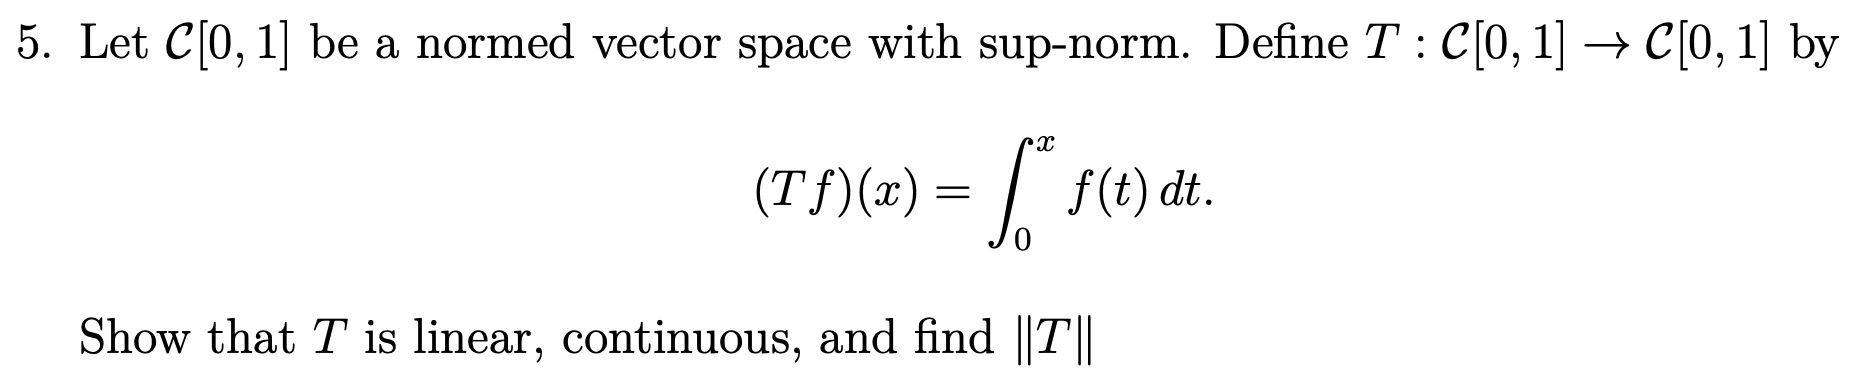
\includegraphics[height=5cm,width=18cm]{ahw4q5}
\end{question}
\begin{proof}
It is quite clear that $T$ is linear. See 
\begin{align*}
  \big(T(f+cg) \big)(x)&=\int_0^x (f+cg)(t)dt\\
  &=\int_0^x f(t)dt + c\int_0^x g(t)dt\\
  &=(Tf+cTg)(x)
\end{align*}
We now show 
\begin{align*}
\vi{\norm{T}_\text{op}=1}
\end{align*}
In other words, we wish to show 
\begin{align*}
  \vi{\sup_{\norm{f}_\infty\leq 1}\norm{Tf}_{\infty}=1}
\end{align*}
Fix 
\begin{align*}
g(x)\triangleq 1
\end{align*}
We see that $\norm{g}_\infty\leq 1$ and 
\begin{align*}
  (Tg)(x)=\int_0^x dt=x
\end{align*}
which implies $\norm{Tg}_{\infty}=1$. This then implies 
\begin{align*}
\sup_{\norm{f}_\infty \leq 1}\norm{Tf}_\infty \geq 1
\end{align*}
We can now reduce the problem into proving 
\begin{align*}
\vi{\sup_{\norm{f}_\infty \leq 1}\norm{Tf}_\infty \leq 1}
\end{align*}
Fix $f\in \mathcal{C}[0,1]$ such that $\norm{f}_\infty\leq 1$. We reduce the problem into proving 
\begin{align*}
  \vi{\norm{Tf}_\infty \leq 1}
\end{align*}
Fix $x \in [0,1]$. We reduce the problem into proving 
\begin{align*}
  \vi{\abso{Tf(x)}\leq 1}
\end{align*}
Observe 
\begin{align*}
\abso{Tf(x)}&=\abso{\int_0^x f(t)dt}\\
&\leq \int_0^x \abso{f(t)}dt\\
&\leq \int_0^x 1dt\hspace{0.5cm}(\because \norm{f}_\infty \leq 1)\\
&=x \leq 1\vdone
\end{align*}
Note that we have shown $T$ is bounded. This implies $T$ is continuous, since $T$ is a linear transformation. (See Question 2) 
\end{proof}
\begin{question}{}{}
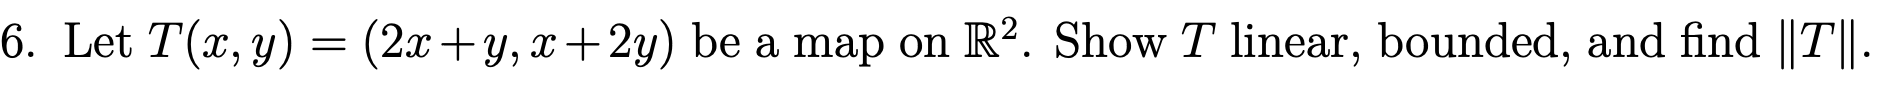
\includegraphics[height=2cm,width=18cm]{ahw4q6}
\end{question}
\begin{proof}
Let $\alpha =\set{\begin{bmatrix}
1\\
0
\end{bmatrix},\begin{bmatrix}
0\\
1
\end{bmatrix}}$. We have
\begin{align*}
[T]_\alpha = \begin{bmatrix}
  2&1\\
  1 & 2
\end{bmatrix}
\end{align*}
Compute the diagonalization 
\begin{align*}
\begin{bmatrix}
T
\end{bmatrix}_{\alpha }= \begin{bmatrix}
1 & 1 \\
1 & -1
\end{bmatrix}\begin{bmatrix}
3 & 0 \\
0 & 1
\end{bmatrix}\begin{bmatrix}
1 & 1 \\
1 & -1
\end{bmatrix}^{-1}
\end{align*}
Let $P,V\in L(\R^2,\R^2)$ satisfy 
\begin{align*}
  [P]_\alpha = \begin{bmatrix}
    1 & 1 \\
    1 & -1
  \end{bmatrix}\text{ and }[V]_\alpha = \begin{bmatrix}
    3 & 0 \\
    0 & 1
  \end{bmatrix}
\end{align*}
Note that $\frac{1}{\sqrt{2}}P$ is an orthogonal transformation. Because orthogonal transformation preserve distance, we see that $\norm{\frac{1}{\sqrt{2}}P}_\text{op}=1$. Because $(\frac{1}{\sqrt{2}}P)^{-1}=\sqrt{2}P^{-1}$ and the invert of an orthogonal transformation is again an orthogonal transformation, we see that $\norm{\sqrt{2}P^{-1}}_\text{op}=1$.\\


Now, from 
\begin{align*}
T=\frac{1}{\sqrt{2}}P\circ V\circ \sqrt{2}P^{-1} 
\end{align*}
We can deduce
\begin{align*}
\norm{T}_{\text{op}}\leq \norm{\frac{1}{\sqrt{2} }P}_{\text{op}}\norm{V}_{\text{op}}\norm{\sqrt{2}P^{-1}}_{\text{op}}= \norm{V}_{\text{op}}
\end{align*}
and deduce 
\begin{align*}
\norm{V}_\text{op}\leq \norm{\sqrt{2}P^{-1}}_\text{op}\norm{T}_\text{op}\norm{\frac{1}{\sqrt{2} }P}_\text{op}= \norm{T}_{\text{op}}
\end{align*}
This give us 
\begin{align*}
\norm{T}_{\text{op}}=\norm{V}_{\text{op}}
\end{align*}
Now consider $\begin{bmatrix}
x\\
y
\end{bmatrix}$ such that $x^2+y^2=1$. We wish to find the maximum of 
 \begin{align*}
\abso{V\begin{bmatrix}
x\\
y
\end{bmatrix}}
\end{align*}
Compute 
\begin{align*}
\abso{V\begin{bmatrix}
x\\
y
\end{bmatrix}}=\sqrt{9x^2+y^2} 
\end{align*}
In other words, we wish to find the maximum of 
\begin{align*}
\sqrt{9x^2+y^2} \text{ when $x^2+y^2=1$ }
\end{align*}
Compute 
\begin{align*}
\sqrt{9x^2+y^2}=\sqrt{1+8x^2} 
\end{align*}
This implies $\sqrt{9x^2+y^2}$ is maximum when $x=\pm 1$ and the value is  $3$.\\

In conclusion,  $\norm{T}_\text{op}=3$. This implies that $T$ is bounded, and further implies that  $T$ is continuous. See Question 2. 
\end{proof}
\begin{question}{}{}
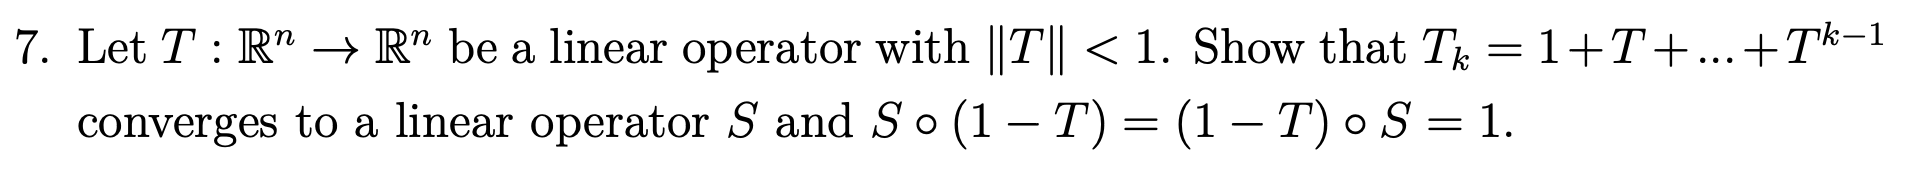
\includegraphics[height=3cm,width=18cm]{ahw4q7}
\end{question}
\begin{proof}
We first show 
\begin{align*}
\vi{T_n\text{ is Cauchy in }\Big(L(\R^n,\R^n),\norm{\cdot}_\text{op} \Big)}
\end{align*}
Note that this suffices, since $\Big(L(\R^n,\R^n), \norm{\cdot}_\text{op} \Big)$ is complete, by Question 1.\\

Fix $\epsilon $. We wish 
\begin{align*}
\vi{\text{ to find }N\text{ such that for all $n>m>N$ we have }\norm{T_n-T_m}_\text{op}\leq \epsilon }
\end{align*}
Because $\norm{T}_{\text{op}}<1$, we see the geometric series 
\begin{align*}
  \sum_{k=0}^{\infty} \norm{T}_{\text{op}}^k\text{ converge }
\end{align*}
Then by direct comparison test ($\norm{T^k}_\text{op}\leq \norm{T}_\text{op}^k$), we know 
\begin{align*}
\sum_{k=0}^{\infty} \norm{T^k}_{\text{op}}\text{ converges, thus Cauchy }
\end{align*}
Then we know 
\begin{align*}
\text{ there exists $N'$ such that for all  $n>m>N'$, we have }\sum_{k=m}^{n-1} \norm{T^{k}}_\text{op}<\epsilon 
\end{align*}
We claim 
\begin{align*}
\vi{\text{ such $N'$ works }}
\end{align*}
Fix $n>m>N'$. Observe 
 \begin{align*}
\norm{T_n-T_m}_\text{op}&=\norm{\sum_{k=m}^{n-1}T^k}_\text{op}\\
&\leq \sum_{k=m}^{n-1} \norm{T^k}_\text{op}\\
&\leq \sum_{k=m}^{n-1} \norm{T}_{\text{op}}^k \leq \epsilon  \vdone
\end{align*}
Now, let $S\triangleq \lim_{k\to \infty}T_k$. Note that $(1-T)\circ S=1 \implies S=(1-T)^{-1}\implies S\circ (1-T)=1$, so it suffices to just prove 
\begin{align*}
\blue{(1-T)\circ S=1}
\end{align*}
Fix $x \inr^n$. We wish to prove 
\begin{align*}
  \blue{(1-T)\lim_{k\to \infty}T_k(x)=x}
\end{align*}
Because we know $\lim_{k\to \infty}T_k(x)$ exists, and $1-T$ is continuous,  (all linear transformation in $\R^n$ is continuous, see \myref{Theorem}{LmoF}), we have
\begin{align*}
  (1-T)\lim_{k\to \infty}T_k(x)=\lim_{k\to \infty}(1-T)T_k(x)
\end{align*}
We can now reduce the problem into proving 
\begin{align*}
  \blue{\lim_{k\to \infty}(1-T)T_k(x)=x}
\end{align*}
Compute 
\begin{align*}
  (1-T)T_k&=T_k-T T_k\\
  &=\sum_{n=0}^{k-1} T^n - \sum_{n=1}^{k} T^n\\
  &=1-T^k
\end{align*}
This let us reduce the problem into 
\begin{align*}
  \blue{\lim_{k\to \infty}T^k(x)=0}
\end{align*}
Fix $r=\norm{T}_{\text{op}}<1$. Observe 
\begin{align*}
\norm{T^k(x)}_{\text{op}}\leq \norm{T}_\text{op}^k \abso{x}=r^k \abso{x} 
\end{align*}
Because $r^k\abso{x}\to 0$ as $k\to \infty$, this implies 
\begin{align*}
  \lim_{k\to \infty}\norm{T^k(x)}=0
\end{align*}
and implies 
\begin{align*}
\lim_{k\to \infty}T^k(x)=0\bdone
\end{align*}


\end{proof}
\begin{question}{}{}
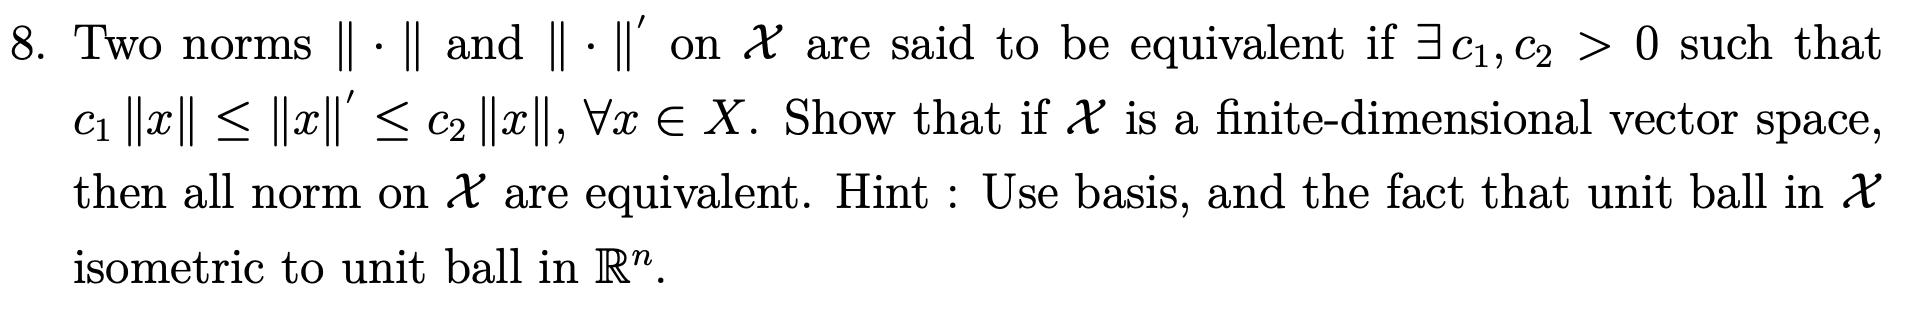
\includegraphics[height=6cm,width=18cm]{ahw4q8}
\end{question}
\begin{proof}
See \myref{Theorem}{ANoF}
\end{proof}
\section{Operator Norm}
\begin{mdframed}
In this section, and particularly in functional analysis, we say a function $T$ between two metric space is a  \textbf{bounded operator} if $T$ always map bounded set to bounded set. In particular, if $T$ is a linear transformation between two normed space, we say $T$ is a \textbf{bounded linear operator}.\\

Suppose $\mathcal{X},\mathcal{Y}$ are two normed space over $\R\text{ or }\C$. In space $L(\mathcal{X},\mathcal{Y})$, alternatively, we can define the boundedness for each linear transformation $T$ by 
\begin{align*}
T\text{ is bounded } \overset{\triangle}{\iff} \exists M\inr,\forall x\in \mathcal{X}, \norm{Tx}\leq M\norm{x}
\end{align*}
The proof of equivalency is simple. For $(\longrightarrow )$,  $E\triangleq \set{y \in \mathcal{X}: \norm{y}=1}$ is non-empty. Clearly, $E$ is bounded. Let $M=\sup_{y\in E} \norm{Ty}$. We now have 
\begin{align*}
\norm{Tx}= \norm{x}\cdot\norm{T \frac{x}{\norm{x}}}\leq M\norm{x}
\end{align*}
For $(\longleftarrow)$, just observe $\norm{Tx-Ty}=\norm{T(x-y)}\leq M\norm{x-y}$.\\


Here, we first show a linear transformation is continuous if and only if it is bounded. (\myref{Theorem}{LOB}) 
\end{mdframed}
\begin{theorem}
\label{LOB}
\textbf{(Liner Operator is Bounded if and only if it is Continuous)} Given two normed space $\mathcal{X},\mathcal{Y}$ over $\R\text{ or }\C$ and  $T\in L(\mathcal{X},\mathcal{Y})$, we have 
\begin{align*}
T\text{ is a bounded operator }\iff T\text{ is continuous on $\mathcal{X}$}
\end{align*}
\end{theorem}
\begin{proof}
$(\longrightarrow)$ We show 
\begin{align*}
\vi{T\text{ is Lipschitz continuous on }V}
\end{align*}
Because $T$ is bounded, we can let $M\inr^+$ satisfy $\norm{Tx}\leq M\norm{x}$. We see 
\begin{align*}
\norm{Tx-Ty}\leq \norm{T(x-y)}\leq M \norm{x-y}\vdone
\end{align*}
$(\longleftarrow)$\\

Because $T$ is linear and continuous at $0$, we know there exists  $\epsilon $ such that 
\begin{align*}
\sup_{\norm{y}\leq \epsilon } \norm{Ty} \leq 1
\end{align*}
We claim 
\begin{align*}
\blue{\hspace{3cm}\norm{Tx}\leq \frac{1}{\epsilon }\norm{x}\hspace{1.5cm}(x\in \mathcal{X})}
\end{align*}
Fix $x\in V$. Compute 
\begin{align*}
\norm{Tx}= \frac{\norm{x}}{\epsilon } \bnorm{T \frac{\epsilon x}{\norm{x}}}\leq \frac{\norm{x}}{\epsilon}\bdone
\end{align*}
\end{proof}
\begin{mdframed}
Here, we introduce a new terminology, which shall later show its value. Given a set $X$, we say two metrics $d_1,d_2$ on $X$ are \textbf{equivalent}, and write $d_1\sim d_2$, if we have 
\begin{align*}
\exists m,M \inr^+, \forall x ,y\in X, md_1(x,y)\leq d_2(x,y) \leq Md_1(x,y)
\end{align*}
Now, given a fixed vector space $V$, naturally, we say two norms $\norm{\cdot}_1,\norm{\cdot}_2$ on $V$ are \textbf{equivalent} if 
\begin{align*}
\exists m,M \inr^+, \forall x\in X, m \norm{x}_1\leq \norm{x}_2 \leq M\norm{x}_1
\end{align*}
We say two metric $d_1,d_2$ on  $X$ are  \textbf{topologically equivalent} if the topology they induce on $X$ are identical.\\

A few properties can be immediately spotted.  
\begin{enumerate}[label=(\alph*)]
  \item Our definition of $\sim$ between metrics of a fixed $X$ is an equivalence relation.
  \item Our definition of $\sim$ between norms on a fixed $V$ is an equivalence relation.
  \item Equivalent norms induce equivalent metrics.
  \item Equivalent metrics are topologically equivalent. 
\end{enumerate}

We now prove that if $V$ is finite-dimensional, then all norms on  $V$ are equivalent (\myref{Theorem}{ANoF}). This property will later show its value, as used to prove that linear map of finite-dimensional domain is alwasy continuous (\myref{Theorem}{LmoF})
\end{mdframed}
\begin{theorem}
\label{ANoF}
\textbf{(All Norms on Finite-dimensional space are Equivalent)} Suppose $V$ is a finite-dimensional vector space over $\R\text{ or }\C$. Then 
\begin{align*}
\text{ all norms on $V$ are equivalent }
\end{align*}
\end{theorem}
\begin{proof}
Let $\set{e_1,\dots ,e_n}$ be a basis of $V$. Define $\infty$-norm $\norm{\cdot}_\infty$ on $V$ by 
\begin{align*}
\norm{\sum \alpha_i e_i}_{\infty}\triangleq  \max \abso{\alpha_i} 
\end{align*}
It is easily checked that $\norm{\cdot}_\infty$ is indeed a norm. Fix a norm $\norm{\cdot}$ on $V$. We reduce the problem into  
\begin{align*}
  \vi{\text{ finding $m,M\inr^+$ such that }m\norm{x}_\infty \leq \norm{x}\leq M\norm{x}_\infty}
\end{align*}
We first claim 
\begin{align*}
\blue{M=\sum \norm{e_i}\text{ suffices }}
\end{align*}
Compute 
\begin{align*}
\norm{x}= \bnorm{\sum \alpha_ie_i} \leq \sum \abso{\alpha _i} \norm{e_i} \leq \norm{x}_\infty \sum \norm{e_i}= M \norm{x}_\infty \bdone
\end{align*}
Reverse triangle inequality give us 
\begin{align*}
\Big|\norm{x}-\norm{y}\Big|\leq \norm{x-y} \leq M \norm{x-y}_\infty
\end{align*}
This implies that $\norm{\cdot}:\Big(V,\norm{\cdot}_\infty \Big)\rightarrow \R$ is Lipschitz continuous.\\


 
Define $S\triangleq \set{y \in V: \norm{y}_\infty =1}$ is non-empty. Check that $S$ is compact in $\norm{\cdot}_\infty$ by checking  $S$ is sequentially compact using the fact $\R^{n-1}$ is locally compact.\\


Now, by EVT, we know $\min _{y \in S}\norm{y}$ exists. Note that $\min_{y \in S}\norm{y}>0$, since $0 \not\in S$.\\ 

We claim 
\begin{align*}
  \olive{m= \min_{y \in S}\norm{y}\text{ suffices }}
\end{align*}
Fix $x \in V$. Compute 
\begin{align*}
m\norm{x}_\infty = \norm{x}_\infty (\min_{y \in S} \norm{y})\leq \norm{x}_\infty \cdot  \bnorm{ \frac{x}{\norm{x}_\infty}}=\norm{x}\odone \vdone
\end{align*}






\end{proof}
\begin{theorem}
\label{LmoF}
\textbf{(Linear map of Finite-dimensional Domain is always Continuous)} Given a finite-dimensional normed space $\mathcal{X}$ over $\R\text{ or }\C$, an arbitrary normed space  $\mathcal{Y}$ over $\R\text{ or }\C$ and a linear transformation  $T:\mathcal{X}\rightarrow \mathcal{Y}$, we have 
\begin{align*}
T\text{ is continuous }
\end{align*}
\end{theorem}
\begin{proof}
Fix $x\in \mathcal{X},\epsilon $. We wish 
\begin{align*}
\vi{\text{ to find $\delta$ such that }\forall h\in \mathcal{X}: \norm{h}\leq \delta, \norm{T(x+h)-Tx}\leq \epsilon }
\end{align*}
Let $\set{e_1,\dots ,e_n}$ be a basis of $\mathcal{X}$. Note that $ \norm{ \sum \alpha_i e_i }_1: = \sum \abso{\alpha _i}$ is a norm. By \myref{Theorem}{ANoF}, we know $\norm{\cdot}$ and $\norm{\cdot}_1$ are equivalent. Then, we can fix $M\inr^+$ such that 
\begin{align*}
\hspace{2cm}\norm{x}_1 \leq M\norm{x}\hspace{0.5cm}(x \in V)
\end{align*}
We claim 
\begin{align*}
\vi{\delta= \frac{\epsilon }{M(\max \norm{Te_i} )}\text{ suffices }} 
\end{align*}
Fix $\norm{h}\leq \delta$ and express $h=\sum \alpha_i e_i$. Compute using linearity of $T$
\begin{align*}
  \norm{T(x+h)-Tx}&=\norm{\sum \alpha_i T e_i}\\
  &\leq \sum \abso{\alpha _i} \norm{Te_i}\\
  &\leq  \norm{h}_1 (\max \norm{Te_i} )\\
  &\leq M \norm{h}(\max \norm{Te_i})\leq \epsilon \vdone
\end{align*}
\end{proof}
\begin{mdframed}
As a corollary of \myref{Theorem}{LOB} and \myref{Theorem}{LmoF}, we now see that, if $\mathcal{X}$ is finite-dimensional, then all linear map of domain $\mathcal{X}$ are bounded. A counter example to the generalization of this statement is followed. 
\begin{Example}{\textbf{(Differentiation is an Unbounded Linear Operator)}}{}
\begin{align*}
\mathcal{X}=\Big(\R[x]|_{[0,1]}, \norm{\cdot}_\infty \Big), D(P)\triangleq P'
\end{align*}
Note that $\set{x^n}_{n\inn}$ is bounded in $\mathcal{X}$ and $\set{D(x^n)}_{n\inn}$ is not.   
\end{Example}
Now, suppose $\mathcal{X},\mathcal{Y}$ are two fixed normed spaces over $\R$ or $\C$. We can easily check that the set $BL(\mathcal{X},\mathcal{Y})$ of bounded linear operators from $\mathcal{X}$ to $\mathcal{Y}$ form a vector space over whichever field $\mathcal{Y}$ is over.\\

Naturally, our definition of boundedness of linear operator derive us a norm on $BL(\mathcal{X},\mathcal{Y})$, as followed 
\begin{align}
\label{tnop}
\norm{T}_{\text{op}}\triangleq \inf \set{M\inr^+ :\forall x \in \mathcal{X}, \norm{Tx}\leq M\norm{x}}
\end{align}
Before we show that our definition is indeed a norm, we first give some equivalent definitions and prove their equivalency. 
\end{mdframed}
\begin{theorem}
\textbf{(Equivalent Definitions of Operator Norm)} Given two fixed normed space $\mathcal{X},\mathcal{Y}$ over $\R$ or  $\C$, a bounded linear operator  $T:\mathcal{X}\rightarrow \mathcal{Y}$, and define $\norm{T}_{\text{op}}$ as in $\hspace{0.5cm}$ (\myref{}{tnop}), we have 
\begin{align*}
\norm{T}_{\text{op}}=\sup_{x\in \mathcal{X},x\neq 0} \frac{\norm{Tx}}{\norm{x}}
\end{align*}
\end{theorem}
\begin{proof}
Define $J=\set{M\inr^+:\forall x \in \mathcal{X},\norm{Tx}\leq M\norm{x}}$, so that we have $\norm{T}_{\text{op}}=\inf J$. Now, observe 
\begin{align*}
J&=\set{M\inr^+:M\geq \frac{\norm{Tx}}{\norm{x}},\forall x\neq 0\in \mathcal{X}}\\
&=\bset{M\inr^+ : M \geq \sup_{x \in \mathcal{X},x\neq 0} \frac{\norm{Tx}}{\norm{x}}}
\end{align*}
This let us conclude 
\begin{align*}
\norm{T}_\text{op}=\inf J=\sup_{x \in \mathcal{X},x\neq 0} \frac{\norm{Tx}}{\norm{x}}
\end{align*}
\end{proof}
\begin{mdframed}
It is now easy to see 
\begin{align}
  \norm{T}_{\text{op}}&=\sup_{x \in \mathcal{X},x\neq 0} \frac{\norm{Tx}}{\norm{x}}\label{equivdefopnorm1}\\
&=\sup_{x\in \mathcal{X},\norm{x}=1} \norm{Tx}\label{equivdefopnorm}
\end{align}
It is not all in vain to introduce the equivalent definitions. See that the verification of  $\norm{\cdot}_{\text{op}}$ being a norm on $BL(\mathcal{X},\mathcal{Y})$ become simple by utilizing the equivalent definitions. 
\begin{enumerate}[label=(\alph*)]
  \item For positive-definiteness, fix non-trivial $T$ and fix $x\in \mathcal{X}\setminus N(T)$. Use (\myref{}{equivdefopnorm1}) to show $\norm{T}_{\text{op}}\geq \frac{\norm{Tx}}{\norm{x}}>0$. 
  \item For absolute homogenity, use (\myref{}{equivdefopnorm}) and $\norm{Tcx}=\abso{c}\cdot \norm{Tx}$.
  \item For triangle inequality, use (\myref{}{equivdefopnorm}) and $\norm{(T_1+T_2)x}\leq \norm{T_1x}+\norm{T_2x}$. 
\end{enumerate}
Naturally, and very very importantly, (\myref{}{equivdefopnorm1}) give us 
\begin{align*}
\hspace{3cm}\norm{Tx}\leq \norm{T}_\text{op}\cdot \norm{x}\hspace{1.5cm}(x\in \mathcal{X})
\end{align*}
This inequality will later be the best tool to help analyze the derivatives of functions between Euclidean spaces, and perhaps better, it immediately give us 
\begin{align*}
 \frac{\norm{T_1T_2x}}{\norm{x}}\leq \frac{\norm{T_1}_\text{op}\cdot \norm{T_2}_\text{op}\cdot \norm{x}}{\norm{x}}=\norm{T_1}_\text{op}\cdot \norm{T_2}_{\text{op}}
\end{align*}
Then (\myref{}{equivdefopnorm1}) give us  
\begin{align*}
\norm{T_1T_2}_\text{op}\leq \norm{T_1}_\text{op}\cdot \norm{T_2}_\text{op}
\end{align*}
\end{mdframed}
\chapter{ODE}
\section{Solution 2}
\begin{mdframed}
1.(a)
\begin{align*}
x^2+2x+2
\end{align*}
1.(b)
\begin{align*}
x
\end{align*}
2.(a)
\begin{align*}
y_P(t)=9te^{2t}+ \frac{-1}{5}\cos t+ \frac{3}{5}\sin t
\end{align*}
2.(b)
\begin{align*}
y_P(t)= \frac{t^3}{6}e^t+t^2+4t+6
\end{align*}
2.(c)
\begin{align*}
y_1=e^t,y_2=e^{-t},y_3=t,y_4=1,y_P=\frac{-t^3}{6}+\frac{t}{2}e^t
\end{align*}
2.(d)
\begin{align*}
\begin{cases}
  y_1=e^t,y_2=te^t, y_3=1,y_4=\cos t, y_5= \sin t\\
  y_P(t)=\frac{t^2}{2}+2t+\frac{t^2}{4}e^t- \frac{t \cos t }{4}
\end{cases}
\end{align*}
3.(a)
\begin{align*}
y_P(t)=\Big(\frac{\sin 2t}{2}-t \Big)\cos t+ \Big(\frac{-\cos 2t}{2} \Big)\sin t
\end{align*}
3.(b)
\begin{align*}
y_P(t)=te^t+(\ln t)te^t
\end{align*}
3.(c)
\begin{align*}
  y_P(x)=\Big(\frac{x}{2}-1 \Big)e^{2x}
\end{align*}
\end{mdframed}
\begin{mdframed}
Summary of the information I gathered: 7 questions. 
\begin{enumerate}[label=(\alph*)]
  \item 3 questions are solving second order homogeneous linear ODE with constant coefficients. i.e. $ay''+by'+cy=0, y(t_0)=y_0, y'(t_0)=y_0'$. The Characteristic polynomials of these 3 questions will respectively have distinct roots, complex roots, and repeated root.
  \item 2 questions are solving second order non-homogeneous linear ODE. Probably, one of them shall be solved by "undetermined coefficients", and another shall be solved by "variation of parameter" 
  \item The last 2 questions are third order (linear) ODE. The method wasn't revealed. 
\end{enumerate}

\end{mdframed}
\chapter{Geometry Archived}
\section{Prerequiste}
\begin{mdframed}
In this section, we will use $I$ to denote an \textbf{bounded open interval}. By a \textbf{curve} in $\R^n$, we mean a function form an open interval $I$ to $\R^n$.  We say a curve is \textbf{differentiable} if it is infinitely differentiable (smooth). That is, $\gamma ^{(n)}(t)$ exists and are continuous for all $n\inn$ and $t \in I$.\\

We say a differentiable curve $\gamma  :I\rightarrow \R^n$ is \textbf{regular} if $\gamma '(t)\neq 0$ for all $t  \in I$. We say a differentiable curve $\gamma :I\rightarrow \R^n$ is a \textbf{parametrized by arc-length} if $\abso{\gamma '(t)}=1$ for all $t \in I$. 
\end{mdframed}
\begin{mdframed}
For a regular curve $\gamma $, we say $\gamma '(t)$ is the \textbf{tangent vector} of $\gamma $ at $t$, and we define the \textbf{unit tangent vector} $T$ by    
\begin{align*}
T(t)\triangleq \frac{\gamma '(t)}{\abso{\gamma '(t)}}
\end{align*}
We say $\gamma ''(t)$ is the \textbf{oriented curvature} (normal vector) of $\gamma $ at $t$, and we define the  \textbf{unit normal vector} $N$ by 
 \begin{align*}
N(t)\triangleq \frac{T'(t)}{\abso{T'(t)}}
\end{align*}
Some interesting facts can be observed from what we have deduced.
\begin{enumerate}[label=(\alph*)]
  \item $\gamma ',\gamma ''$ always exists. 
  \item $\gamma $ is parametrized by arc-length $\implies \gamma ' \perp \gamma ''$
  \item $\gamma $ is parametrized by arc-length $\implies \gamma $ is regular
  \item $T$ and $T'$ exists at $t$  $\iff $ $\gamma $ is regular at $t$ 
  \item $T=\gamma '\iff \gamma $ is parametrized by arc-length   
  \item $N$ exists at $t$ $\iff \gamma ''(t)\neq 0\iff  \kappa (t)\neq 0$  
  \item $N$ and  $T'$ point to the same direction $\gamma ''$.
  \item $\abso{T'}=\kappa\iff \gamma $ is paramterized by arc-length 
  \item $\gamma \perp \gamma '$ and $\gamma'' \perp \gamma '''$ are generally false even for curve $\gamma $ paramterized by arc-length. 
  \item Given a curve $\gamma $ parametrized by arc-length
\begin{align*}
  \gamma \text{ is a straight line on }[a,b]&\iff  \gamma '\text{ and }T\text{ are constant on $(a,b)$ }\\
  &\iff \gamma ''(t)=0\text{ on $(a,b)$ }\\
  &\iff \kappa (t)=0\text{ on $(a,b)$ }\\
  &\iff T'(t)=0\text{ on }(a,b)
\end{align*}
\end{enumerate}
Notice that the last fact is false if $\gamma $ is not paramtetrized by arc-length, since $\gamma $ can move in the straight line with changing speed $\gamma '$.  
\end{mdframed}

\begin{mdframed}
Given a curve $\gamma $, if $T(t)$ and $N(t)$ exists (regular and non-zero curvature), we define its \textbf{binormal} vector by 
\begin{align*}
B(t)=T(t) \times N(t)
\end{align*}
Fix $t$. We say 
\begin{align*}
\set{T(t),N(t),B(t)}\text{ form a \textbf{positively oriented orthonormal basis} of $\R^3$ }
\end{align*}
This basis in general is constantly changing, yet always form an orthonormal basis.\\

Also, we say 
\begin{align*}
\text{span}\Big( T(t),N(t)\Big)\text{ is the \textbf{osculating plane} of $\gamma $ at $t$ }
\end{align*}
Suppose $\gamma $ is parametrized by arc-length and always has non-zero curvature. With some geometric intuition, one shall note that $\abso{T'}$ measure how curved $\gamma $ is and that $\abso{B'}$ measure how fast  $\gamma $ leave the osculating plane.\\

Because $\abso{B}=1$ is a constant, we can deduce  
\begin{align*}
B'\perp B
\end{align*}
and the computation 
\begin{align*}
B'=T' \times N + T \times N'=T \times N' 
\end{align*}
give us 
\begin{align*}
B'\perp T
\end{align*}
This ultimately show us 
\begin{align*}
B',N,T'\text{ are all parallel where $N,T'$ even point to the same direction}
\end{align*}


Notice that if we parametrize the curve with opposite direction, then 
\begin{enumerate}[label=(\alph*)]
  \item $T,\gamma '$ change direction 
  \item $N,\gamma ''$ keep the same direction 
  \item $B$ change direction 
  \item $B'$ keep the same direction 
\end{enumerate}
Now, for a curve $\gamma $ parametrized by arc-length, we define the \textbf{curvature} $\kappa$ and \textbf{torsion} $\tau$ of $\gamma $ by 
\begin{align*}
\kappa(t)=\abso{\gamma ''(t)}\text{ and }\tau (t)=\frac{B'(t)}{N(t)}
\end{align*}
With unfortunately heavy computation, we can verify that the definition of curvature must stay in the framework of curve parametrized by arc-length, otherwise we will be given two different values of curvature of two curves that are equivalent in the sense of sets.\\

Now, notice that we already have $T'=\kappa N$ and $B'=\tau N$, and by basic identity, we have $N=B\times T$.\\

Then $\underline{\text{with some computation}}$, we have the \textbf{Frenet Formula}
\begin{align*}
\begin{cases}
  T'=\kappa N\\
  N'=B'\times T+B\times T'=-\tau B-\kappa T\\
  B'=\tau N
\end{cases}
\end{align*}
\end{mdframed}
\begin{mdframed}
Given two vectors $u,v \inr^n$, we use  \textbf{dot product} 
\begin{align*}
u\cdot v= u_1v_1+\cdots + u_nv_n
\end{align*}
to denote the Euclidean inner product, and we use \textbf{length} 
\begin{align*}
\abso{u}=\sqrt{\sum_{k=1}^n u_k^2} 
\end{align*}
to denote the Euclidean norm. Note that we clearly have 
\begin{align*}
\abso{u}=\sqrt{u\cdot u} 
\end{align*}
Given three vectors $u,v,w \inr^3$, we define \textbf{cross product} by 
\begin{align*}
  u\times v&\triangleq \begin{vmatrix} 
  \textbf{i} & \textbf{j} & \textbf{k}\\
  u_1 & u_2 & u_3 \\
  v_1 & v_2 & v_3
\end{vmatrix}\\
&=(u_2v_3-u_3v_2,u_3v_1-u_1v_3,u_1v_2-u_2v_1)
\end{align*}
With some simple computation, we have the following identity 
\begin{enumerate}[label=(\alph*)]
  \item $u\times v=-v \times u$ (anti-commutative)
  \item $(au+w)\times v=a(u\times v)+w \times v$ (Linearity)
  \item $u\times (aw+v)=a (u\times w)+ u \times v$
  \item $u \times v =0 \iff u=cv$ for some $c \inr$
  \item $(u\times v)\cdot w =\begin{vmatrix} 
      u_1 & u_2 & u_3 \\
      v_1 & v_2 & v_3 \\
      w_1 & w_2 & w_3   \end{vmatrix}=\begin{vmatrix}
      w_1 & w_2 & w_3 \\
      u_1 & u_2 & u_3 \\
      v_1 & v_2 & v_3 
  \end{vmatrix}$ 
  \item $(u \times v)\cdot v=0=(u \times v)\cdot u$
  \item $u \times v \perp u$ and $u\times v\perp v$
  \item $u \perp v \implies  \abso{u \times v}= \abso{u}\cdot \abso{v}$
  \item $(u \times v)\times w=(u \cdot w)v-(v \cdot w)u$
\end{enumerate}
All proofs except that of the last identity are merely manipulation of determinant. A simple proof of the last identity follows from the fact both side are linear in all $u,v,w$, and the observation 
\begin{align*}
  (e_1\times e_2)\times e_3=0=(e_1\cdot e_3)e_2-(e_2\cdot e_3)e_1
\end{align*}
\end{mdframed}
\begin{theorem}
\textbf{(Differentiate the Dot Product)} Given two parametrized curves $u,v:(a,b)\rightarrow \R^n$, such that $u,v$ are differentiable at  $t \in (a,b)$. We have 
\begin{align*}
\frac{d}{dt}\big(u(t)\cdot v(t) \big)= u'(t)\cdot v(t)+u(t)\cdot v'(t)
\end{align*}
\end{theorem}
\begin{proof}
\begin{align*}
\frac{d}{dt}\big(u(t)\cdot v(t) \big)&=\frac{d}{dt}\sum_{k=1}^n u_k(t)v_k(t)\\
&=\sum_{k=1}^n \frac{d}{dt} u_k(t)v_k(t)\\
&=\sum_{k=1}^n u_k'(t)v_k(t)+u_k(t)v_k'(t)\\
&=\sum_{k=1}^n u_k'(t)v_k(t)+\sum_{k=1}^n u_k(t)v_k'(t)\\
&=u'(t)\cdot v(t)+u(t)\cdot v'(t)
\end{align*}
\end{proof}
\begin{theorem}
\textbf{(Differentiate the Cross Product)} Given two curves $u,v:(a,b)\rightarrow \R^3$, such that $u,v$ are differentiable at  $t \in (a,b)$. We have 
\begin{align*}
\frac{d}{dt}\big(u (t)\times v(t) \big)=u'(t)\times v(t)+u(t)\times v'(t)
\end{align*}
\end{theorem}
\begin{proof}
\begin{align*}
  \frac{d}{dt}\big(u(t)\times v(t) \big)=&\frac{d}{dt}(u_2v_3-u_3v_2,u_3v_1-u_1v_3,u_1v_2-u_2v_1)\\
=&(u_2'v_3+u_2v_3'-u_3'v_2-u_3v_2',\\
 & u_3'v_1+u_3v_1'-u_1'v_3-u_1v_3',\\
 &u_1'v_2+u_1v_2'-u_2'v_1-u_1v_2')\\
=&(u_2'v_3-u_3'v_2,u_3'v_1-u_1'v_3,u_1'v_2-u_2'v_1)\\
+&(u_2v_3'-u_3v_2',u_3v_1'-u_1v_3',u_1v_2'-u_1v_2')\\
=&u'\times v+u \times v'
\end{align*}
\end{proof}
\begin{theorem}
\textbf{(Integrating the Dot Product)} Given a curve $u:[a,b]\rightarrow \R^n$ and a vector $v \in\R^n$, suppose 
\begin{enumerate}[label=(\alph*)]
  \item $u$ is differentiable on $(a,b)$ 
  \item $u$ is continuous on  $[a,b]$
\end{enumerate}
We have 
\begin{align*}
\int_a^b u'(t)\cdot v dt=
\Big(\int_a^b u'(t)dt \Big)\cdot v= \big(u(b)-u(a) \big)\cdot v
\end{align*}
\end{theorem}
\begin{proof}
\begin{align*}
\int_a^b u'(t)\cdot vdt&=\int_a^b \sum_{k=1}^n u'_k(t)\cdot v_k dt \\
&=\sum_{k=1}^n  \int_a^b u'_k(t)\cdot v_k dt\\
&=\sum_{k=1}^n v_k \int_a^b u'_k(t)dt\\
&=v\cdot \Big(\int_a^b u'(t)dt \Big)
\end{align*}
\end{proof}
\begin{mdframed}
For the result above, sometimes we write 
\begin{align*}
  (u\cdot v)'=u'\cdot v+ u \cdot v'\text{ and }(u\times v)'=u' \times v+u\times v'
\end{align*}
\end{mdframed}
\begin{theorem}
\textbf{(MVT for curve)} Given a curve $\alpha  : [a,b]\rightarrow \R^n$ such that 
\begin{enumerate}[label=(\alph*)]
  \item $\alpha  $ is differentaible on $(a,b)$ 
  \item $\alpha  $ is continuous on $[a,b]$
\end{enumerate}
there exists $ \xi  \in (a,b)$ such that 
\begin{align*}
\abso{\alpha  (b)-\alpha  (a)}\leq \abso{\alpha  '(\xi  )}(b-a)
\end{align*}
\end{theorem}
\begin{proof}
Define $\phi:[a,b]\rightarrow \R$ by 
\begin{align*}
\phi(t)=\alpha (t)\cdot \big(\alpha (b)-\alpha (a) \big) 
\end{align*}
Clearly $\phi$ satisfy the hypothesis of Lagrange's MVT, then we know there exists $\xi \in (a,b)$ such that 
\begin{align*}
\phi(b)-\phi (a)=\phi'(\xi )\cdot (b-a)
\end{align*}
Written the equation in $\alpha $, we have 
\begin{align*}
\abso{\alpha (b)-\alpha (a)}^2= (b-a)\alpha '(\xi)\cdot \big(\alpha (b)-\alpha (a) \big)
\end{align*}
Notice that Cauchy-Schwarz inequality give us 
\begin{align*}
  (b-a)\abso{\alpha '(\xi)}\cdot \abso{\alpha (b)-\alpha (a)}&\geq (b-a)\abso{\alpha ' (\xi)\cdot \big(\alpha (b)-\alpha (a) \big)} \\
  &=\abso{\alpha (b)-\alpha (a)}^2
\end{align*}
This then implies 
\begin{align*}
  (b-a)\abso{\alpha '(\xi)}\geq \abso{\alpha (b)-\alpha (a)}
\end{align*}
\end{proof}
\begin{corollary}
\label{MVI}
\textbf{(Mean Value Inequality)} Given a curve $\alpha :[a,b]\rightarrow \R^n$ such that 
\begin{enumerate}[label=(\alph*)]
  \item $\alpha $ is differentiable on $(a,b)$ 
  \item $\alpha $ is continuous on $[a,b]$
\end{enumerate}
we have 
\begin{align*}
\abso{\alpha (b)-\alpha (a)}\leq (b-a)\sup_{(a,b)}\abso{\alpha '}
\end{align*}
\end{corollary}
\begin{mdframed}
\textbf{Trick to parametrize by arc-length}.\\

Given a regular curve $\gamma :I\rightarrow \R^n$ and fix $t_0 \in I$. We use
\begin{align*}
  s(t)=\int_{t_0}^t \abso{\gamma  ' (x)}dx
\end{align*}
to define the arc-length of  $\gamma $ from $\gamma (t_0)$ to $\gamma (t)$. Because $\gamma $ is regular, by FTC, it is clear that $s$ is one-to-one.\\

Let $t(s)$ be the inverse of $s$. Define 
 \begin{align*}
\beta (s)\triangleq \alpha (t(s))
\end{align*}
We have by Chain rule 
\begin{align*}
\beta '(s)&=t'(s)\alpha '(t(s))\\
&=\frac{\alpha '(t(s))}{s'(t)}\\
&=\frac{\alpha '(t(s))}{\abso{\alpha '(t(s))}}
\end{align*}
\end{mdframed} 
\begin{mdframed}
\textbf{(Frenet Formula Summary)} \\

By definition, we are given 
\begin{align*}
\begin{cases}
  T'=\kappa N\\
  B'=\tau N
\end{cases}
\end{align*}
To compute $N'$, an identity should be first given 
 \begin{align*}
N=B\times T
\end{align*}
We can now complete the Frenet Formula 
\begin{align*}
N'&=B'\times T + B \times T'\\
&=\tau N \times T + B \times \kappa N\\
&=-\tau B-\kappa T
\end{align*}
In conclusion 
\begin{align*}
\begin{cases}
  T'=\kappa N
  B' =\tau N\\
  N'=-\tau B-\kappa T
\end{cases}
\end{align*}
Give very close attention to the fact the two definitions of curvature 
\begin{align*}
\kappa =\frac{T'}{N}\text{ and }\kappa = \abso{\gamma ''}
\end{align*}
coincides $\underline{\text{only when }}\gamma $ is parametrzied by arc-length. The first definition remain same for all parametrizaiton of the same curve, while the latter doesn't.\\

Some comment should be dropped for the computation of torsion. If you overlook the fact $\alpha $ is parametrized by arc-length and disregard Frenet Formula, it is very likely you will get a result that you can not even sure if it is valid (the nominator and denominator may end up not seem explicitly parallel), let alone an identity beautiful as below. 
\end{mdframed}
\section{Examples of Regular Surfaces}
\begin{mdframed}
Among all regular surfaces, the most classic one is perhaps the $S^2$. Here, we show some local parametriatoin of $S^2$.\\


Note that because  $S^2=F^{-1}[0]$, where $F(x,y,z)=x^2+y^2+z^2-1$ clearly has non-zero derivative everywhere on $\R^3 \setminus 0$, we know $S^2$ is a regular surface. 
\end{mdframed}
\begin{mdframed}
\begin{Example}{\textbf{(Graph Coordinates of $S^2$)}}{}
\begin{align*}
U=\set{(u,v):u^2+v^2<1}\text{ and }S^2=\set{(x,y,z):x^2+y^2+z^2=1}
\end{align*}
\begin{enumerate}[label=(\alph*)]
    \item $f_1:B_{1}(0)\subseteq \R^2 \rightarrow \R^3$ by $f_1(x,y)=(x,y,\sqrt{1-x^2-y^2})$  
    \item $f_2:B_{1}(0)\subseteq \R^2 \rightarrow \R^3$ by $f_2(x,y)=(x,y,-\sqrt{1-x^2-y^2})$  
    \item $f_3:B_{1}(0)\subseteq \R^2 \rightarrow \R^3$ by $f_3(x,z)=(x,\sqrt{1-x^2-z^2},z)$  
    \item $f_4:B_{1}(0)\subseteq \R^2 \rightarrow \R^3$ by $f_4(x,z)=(x,-\sqrt{1-x^2-z^2},z)$  
    \item $f_5:B_{1}(0)\subseteq \R^2 \rightarrow \R^3$ by $f_5(y,z)=(\sqrt{1-y^2-z^2},y,z)$  
    \item $f_6:B_{1}(0)\subseteq \R^2 \rightarrow \R^3$ by $f_6(y,z)=(-\sqrt{1-y^2-z^2},y,z)$  
\end{enumerate}
\end{Example}  
\begin{Example}{\textbf{(Spherical Coordinates of $S^2$)}}{}
\begin{align*}
S^2=\set{(x,y,z):x^2+y^2+z^2=1}
\end{align*}
\begin{enumerate}[label=(\alph*)]
  \item $\textbf{x}_1:(0,\pi)\times (0,2\pi)\rightarrow S^2 $ by $\textbf{x}_1(\theta,\phi)=(\sin \theta \cos \phi,\sin \theta \sin \phi,\cos \theta)$
  \item $\textbf{x}_2:(0,\pi)\times (0,2\pi)\rightarrow S^2$ by $\textbf{x}_2(\theta,\phi)=(-\sin \theta\cos \phi  ,\cos \theta,\sin \theta \sin \phi )$
\end{enumerate}
Note that 
\begin{enumerate}[label=(\alph*)]
  \item $\textbf{x}_1$ does not contain $\set{(x,0,z)\in S^2: \begin{cases}
    x^2+z^2=1\\
    x\geq 0
  \end{cases}}$ 
\item $\textbf{x}_2$ does not contain $\set{(x,y,0)\in S^2: \begin{cases}
  x^2+y^2=1\\
  x\leq 0
\end{cases}}$
\end{enumerate}
\end{Example}

\begin{Example}{\textbf{(Stereographical Coordinates of $S^2$: Projection Plane be the Equator)}}{}
\begin{align*}
U=\R^2\text{ and }S^2=\set{(x,y,z):x^2+y^2+z^2=1}
\end{align*}
Note that
\begin{enumerate}[label=(\alph*)]
  \item $\textbf{x}_N^{-1}(x,y,z)\equiv (\frac{x}{1-z},\frac{y}{1-z})$ 
  \item $\textbf{x}_S^{-1}(x,y,z)\equiv (\frac{x}{z+1},\frac{y}{z+1}) $
\end{enumerate}
For explicit expression of $\textbf{x}_N$, Use the trick 
\begin{align*}
u^2+v^2=\frac{x^2+y^2}{(1-z)^2}=\frac{1-z^2}{(1-z)^2}\text{ and }x=u(1-z),y=v(1-z)
\end{align*}
to first solve for $z$, then solve for $x,y$.\\

Now, we have 
\begin{enumerate}[label=(\alph*)]
  \item $\textbf{x}_N(u,v)=\big(\frac{2u}{u^2+v^2+1},\frac{2v}{u^2+v^2+1},\frac{u^2+v^2-1}{u^2+v^2+1} \big)$
  \item $\textbf{x}_S(u,v)=\big(\frac{2u}{u^2+v^2+1},\frac{2v}{u^2+v^2+1},\frac{1-u^2-v^2}{1+u^2+v^2} \big)$
\end{enumerate}
Let
\begin{align*}
\textbf{x}_N(u,v)=(x,y,z)
\end{align*}
Compute 
\begin{align*}
  \frac{\partial (x,y)}{\partial (u,v)}&=\frac{4(-u^2 - v^2 + 1)}{u^6 + 3u^4v^2 + 3u^4 + 3u^2v^4 + 6u^2v^2 + 3u^2 + v^6 + 3v^4 + 3v^2 + 1}\\
  \frac{\partial (y,z)}{\partial (u,v)}&=\frac{-8u}{u^6 + 3u^4v^2 + 3u^4 + 3u^2v^4 + 6u^2v^2 + 3u^2 + v^6 + 3v^4 + 3v^2 + 1}\\
  \frac{\partial (x,z)}{\partial (u,v)}&=\frac{8v}{u^6 + 3u^4v^2 + 3u^4 + 3u^2v^4 + 6u^2v^2 + 3u^2 + v^6 + 3v^4 + 3v^2 + 1}
\end{align*}
This shows $\textbf{x}_N$ is indeed a local parametrization.   
\end{Example}
Note that 
\begin{align*}
\textbf{x}^{-1}_S \circ \textbf{x}_N (u,v)=\big( \frac{u}{u^2+v^2},\frac{v}{u^2+v^2}\big)
\end{align*}
is a diffeomorphism on $\R^2\setminus 0$, since $\text{det}\Big( d(\textbf{x}_S^{-1}\circ \textbf{x}_N)\Big)=\frac{-1}{(u^2+v^2)^2}$.\\

Also, note that if we identify $(u,v)\equiv u+iv\triangleq \xi$, we have 
\begin{align*}
\textbf{x}_S^{-1}\circ \textbf{x}_N (\xi)=\frac{\xi}{\abso{\xi}^2}
\end{align*}
\end{mdframed}
\begin{mdframed}
\begin{Example}{\textbf{(Stereographical Coordinates of $S^2$: Projection Plane at the Bottom)}}{}
\begin{align*}
U=\R^2\text{ and }S^2=\set{(x,y,z):x^2+y^2+z^2}
\end{align*}
\end{Example}
\end{mdframed}

\end{document}
